%%%%%%%% ICML 2025 EXAMPLE LATEX SUBMISSION FILE %%%%%%%%%%%%%%%%%

\documentclass{article}

% Recommended, but optional, packages for figures and better typesetting:
\usepackage{microtype}
\usepackage{graphicx}
\usepackage{subfigure}
\usepackage{booktabs} % for professional tables
\usepackage{multirow}
\usepackage{bm}
\usepackage{xcolor}
\usepackage{amsmath}
\usepackage{amsthm}
% \usepackage{subcaption}
% \newcommand{\changed}[1]{\textcolor{blue}{#1}}
% \newcommand{\todo}[1]{\textcolor{red}{#1}}
\newtheorem{hypothesis}{Hypothesis}
\usepackage{caption}
\usepackage{float} 
%\usepackage{subfigure}
% \usepackage{subcaption}
\usepackage{amsmath,amssymb,amsfonts}
\usepackage{algorithmic}
\usepackage{textcomp}
\usepackage{bm}
\usepackage{amsfonts}
\usepackage{xcolor}
\usepackage{diagbox}
\usepackage{booktabs}
\usepackage[normalem]{ulem}
\usepackage{multirow}
\usepackage{pifont}
\usepackage{enumitem}

% \usepackage[linesnumbered,ruled,vlined]{algorithm2e}
\usepackage[ruled,vlined]{algorithm2e}
\usepackage{amsmath}
\usepackage{graphicx}

\newcommand{\cmark}{\textcolor{green!50!black}{\ding{51}}}
\newcommand{\xmark}{\textcolor{red}{\ding{55}}}
\newcommand{\neutral}{\textcolor{blue!50!white}{\ding{108}}}

% hyperref makes hyperlinks in the resulting PDF.
% If your build breaks (sometimes temporarily if a hyperlink spans a page)
% please comment out the following usepackage line and replace
% \usepackage{icml2025} with \usepackage[nohyperref]{icml2025} above.
\usepackage{hyperref}


% Attempt to make hyperref and algorithmic work together better:
\newcommand{\theHalgorithm}{\arabic{algorithm}}

% Use the following line for the initial blind version submitted for review:
% \usepackage{icml2025}

% If accepted, instead use the following line for the camera-ready submission:
\usepackage[accepted]{icml2025}

% For theorems and such
\usepackage{amsmath}
\usepackage{amssymb}
\usepackage{mathtools}
\usepackage{amsthm}
\usepackage{colortbl}
\usepackage{tikz}      % 用于绘制图形
\usepackage{colortbl}
\usepackage{float}
\usepackage{listings}
\lstset{
    language=Python,              % 设置语言为 Python
    basicstyle=\rmfamily\small,   % 基础字体样式
    keywordstyle=\color{red},    % 关键词颜色
    commentstyle=\color{green!50!black},    % 注释颜色
    frame=single,                 % 添加边框
    breaklines=true,              % 自动换行
    tabsize=4                     % Tab 键大小
}

% \definecolor{background}{RGB}{245,245,245} % 背景色
% \definecolor{keyword}{RGB}{183,72,182}     % 关键词颜色
% \definecolor{string}{RGB}{196,26,22}       % 字符串颜色
% \definecolor{comment}{RGB}{0,128,0}        % 注释颜色
% \definecolor{variable}{RGB}{51,51,255}     % 变量颜色
% \definecolor{number}{RGB}{170,13,145}      % 数字颜色

% % 自定义minted样式
% \lstset{
%     language=Python,
%     bgcolor=background,          % 背景色
%     frame=lines,                 % 边框
%     framesep=2mm,                % 边框和内容间距
%     linenos,                     % 显示行号
%     numbersep=5pt,               % 行号间距
%     fontfamily=tt,               % 等宽字体
%     fontsize=\small,             % 字体大小
%     xleftmargin=10pt,            % 左边距
%     breaklines=true,             % 自动换行
%     tabsize=4,                   % Tab 大小
%     keywordstyle=\color{keyword},% 关键词颜色
%     stringstyle=\color{string},  % 字符串颜色
%     commentstyle=\color{comment},% 注释颜色
%     numberstyle=\tiny\color{gray}, % 行号样式
% }

% if you use cleveref..
\usepackage[capitalize,noabbrev]{cleveref}

%%%%%%%%%%%%%%%%%%%%%%%%%%%%%%%%
% THEOREMS
%%%%%%%%%%%%%%%%%%%%%%%%%%%%%%%%
\theoremstyle{plain}
\newtheorem{theorem}{Theorem}[section]
\newtheorem{proposition}[theorem]{Proposition}
\newtheorem{lemma}[theorem]{Lemma}
\newtheorem{corollary}[theorem]{Corollary}
\theoremstyle{definition}
\newtheorem{definition}[theorem]{Definition}
\newtheorem{assumption}[theorem]{Assumption}
\theoremstyle{remark}
\newtheorem{remark}[theorem]{Remark}
% \usepackage{ulem}

% Todonotes is useful during development; simply uncomment the next line
%    and comment out the line below the next line to turn off comments
%\usepackage[disable,textsize=tiny]{todonotes}
\usepackage[textsize=tiny]{todonotes}


% The \icmltitle you define below is probably too long as a header.
% Therefore, a short form for the running title is supplied here:
\icmltitlerunning{}


\begin{document}

\twocolumn[
\icmltitle{Harmony in Divergence: Towards Fast, Accurate, and Memory-efficient Zeroth-order LLM Fine-tuning}

% It is OKAY to include author information, even for blind
% submissions: the style file will automatically remove it for you
% unless you've provided the [accepted] option to the icml2025
% package.

% List of affiliations: The first argument should be a (short)
% identifier you will use later to specify author affiliations
% Academic affiliations should list Department, University, City, Region, Country
% Industry affiliations should list Company, City, Region, Country

% You can specify symbols, otherwise they are numbered in order.
% Ideally, you should not use this facility. Affiliations will be numbered
% in order of appearance and this is the preferred way.
\icmlsetsymbol{equal}{*}

\begin{icmlauthorlist}
\icmlauthor{Qitao Tan}{uga}
\icmlauthor{Jun Liu}{neu}
\icmlauthor{Zheng Zhan}{neu}
\icmlauthor{Caiwen Ding}{umt}
\icmlauthor{Yanzhi Wang}{neu}
\icmlauthor{Jin Lu}{uga}
\icmlauthor{Geng Yuan}{uga}
\end{icmlauthorlist}

\icmlaffiliation{uga}{University of Georgia}
\icmlaffiliation{neu}{Northeastern University}
\icmlaffiliation{umt}{University of Minnesota Twin Cities}

\icmlcorrespondingauthor{Geng Yuan}{geng.yuan@uga.edu}
% \icmlcorrespondingauthor{Firstname2 Lastname2}{first2.last2@www.uk}

% You may provide any keywords that you
% find helpful for describing your paper; these are used to populate
% the "keywords" metadata in the PDF but will not be shown in the document
\icmlkeywords{Machine Learning, ICML}

\vskip 0.3in
]

% this must go after the closing bracket ] following \twocolumn[ ...

% This command actually creates the footnote in the first column
% listing the affiliations and the copyright notice.
% The command takes one argument, which is text to display at the start of the footnote.
% The \icmlEqualContribution command is standard text for equal contribution.
% Remove it (just {}) if you do not need this facility.

%\printAffiliationsAndNotice{}  % leave blank if no need to mention equal contribution
\printAffiliationsAndNotice{\icmlEqualContribution} % otherwise use the standard text.


\begin{abstract}
% Large language models (LLMs) demonstrate exceptional performance across a variety of tasks, yet standard first-order (FO) fine-tuning requires considerable memory, significantly limiting practical deployment. 
% Recently, zeroth-order (ZO) optimization stood out as a promising memory-saving training paradigm, foregoing memory-intensive backward passes and estimating gradients solely through forward passes, offering an attractive solution for resource-constrained scenarios. 
Large language models (LLMs) excel across various tasks, but standard first-order (FO) fine-tuning demands considerable memory, significantly limiting real-world deployment. Recently, zeroth-order (ZO) optimization stood out as a promising memory-efficient training paradigm, avoiding backward passes and relying solely on forward passes for gradient estimation, making it attractive for resource-constrained scenarios. However, ZO method lags far behind FO method in both convergence speed and accuracy. To bridge the gap, we introduce a novel layer-wise divergence analysis that uncovers the distinct update pattern of FO and ZO optimization. Aiming to resemble the learning capacity of FO method from the findings, we propose \textbf{Di}vergence-driven \textbf{Z}eroth-\textbf{O}rder (\textbf{DiZO}) optimization. DiZO conducts divergence-driven layer adaptation by incorporating projections to ZO updates, generating diverse-magnitude updates precisely scaled to layer-wise individual optimization needs. Our results demonstrate that DiZO significantly reduces the needed iterations for convergence without sacrificing throughput, cutting training GPU hours by up to 48\% on various datasets. Moreover, DiZO consistently outperforms the representative ZO baselines in fine-tuning RoBERTa-large, OPT-series, and Llama-series on downstream tasks and, in some cases, even surpasses memory-intensive FO fine-tuning.
% Large language models (LLMs) excel in many tasks, but the memory-intensive first-order (FO) fine-tuning greatly limits real-world deployment. In contrast, zeroth-order (ZO) optimization, a promising approach that estimates gradients using only forward passes, significantly reduces memory burden, making it an attractive solution for memory-constrained applications. However, an obvious accuracy and convergence speed gap still exists between these methods and the FO methods. In this work, we first introduce a novel distance-based analysis to investigate the difference in training dynamics between FO and ZO. Aiming to resemble the learning capacity of FO from the findings, we propose \textbf{P}rojection-\textbf{e}nhanced \textbf{Z}eroth-\textbf{O}rder (\textbf{PeZO}) optimization. PeZO conducts projection to the updates from ZO steps, generating customized updates precisely scaled to layer-wise individual optimization needs. Our results demonstrate that PeZO significantly reduces the needed iterations for convergence, cutting GPU hours by up to 48\% on a broad range of datasets, all without sacrificing throughput. Moreover, PeZO consistently outperforms the representative ZO method in fine-tuning RoBERTa, OPT, and Llama on various downstream tasks, achieving superior accuracy.
\end{abstract}

\section{Introduction}



Fine-tuning pre-trained large language models (LLMs) with backpropagation demonstrates
superior performance for many natural language processing tasks~\cite{yang2019end, liu2019roberta,talmor2018commonsenseqa,chowdhery2023palm,zheng2020end}. However, the extensive parameterization imposes a substantial memory burden, limiting their practicality for widespread downstream applications.
% Fine-tuning pre-trained large language models (LLMs) is the state-of-the-art approach for many natural language processing tasks. However, the extensive parameterization and high computational costs have become significant constraints in wide applications. 
In line with the neural scaling laws~\cite{hoffmann2022empirical,kaplan2020scaling}, next-generation LLMs continue to increase in parameter count. Specifically, model sizes are expanding at a rate of 410× every two years, dramatically outpacing the scaling of DRAM bandwidth (1.4× every two years) and DRAM capacity (2× every two years). This disparity leads to the \emph{memory wall} challenge~\cite{gholami2024ai}, which becomes even more severe when deploying LLMs on memory-limited devices~\cite{zeng2024flightllm,chen2024understanding,hur2023fast}.

Recently, zeroth-order (ZO) optimization has emerged as a promising memory-efficient training paradigm for LLM fine-tuning, attracting significant attention~\cite{zhang2024revisiting,liu2024sparse,malladi2023fine, zhao2024second}.
By relying solely on forward passes (i.e., inference) to estimate gradients and update model parameters, ZO bypasses the need for backward propagation and significantly reduces extensive storage requirements for activations, gradients, and optimizer states.
% This method intends only to use forward passes (i.e., inference) to estimate the gradients and update the weights accordingly.
% By completely avoiding the computation of backward propagation, ZO simplifies the computation process and eliminates the need for storing extensive data, including activations, gradients, and optimizer state. 
As reported in~\citet{malladi2023fine}, fine-tuning LLMs via ZO optimization reduces up to 12$\times$ memory cost.
Nevertheless, ZO optimization still exhibits a \textbf{gap} in convergence speed and accuracy compared to the conventional first-order (FO) method (i.e., compute gradient via backpropagation). As shown in Table~\ref{table1}, one can observe that the FO method substantially outperforms ZO method in both accuracy and GPU hours. Though ZO method achieves higher throughput due to its computational simplicity, it requires more than 10× iterations for convergence, dramatically increasing GPU hours. Previous studies typically attribute this gap to the fact that ZO optimization leverages random perturbation for gradient estimation, and thus results in unavoidable estimation error, but without further exploration of other underlying causes~\cite{malladi2023fine, gautam2024variance, zhao2024second}. 


% \begin{table}[t]
% \centering
% \scalebox{0.78}{
% \begin{tabular}{lccccc}
% \toprule
% Model                      & \textbf{Type} & \textbf{Acc} & \textbf{Throughput} & \textbf{Iteration} & \textbf{GPU hours} \\ \hline
% \multirow{2}{*}{RoBERTa-L} & FO   & 91.9 & 2.32 it/s  & 6.6\%     & 12.3\%    \\
%                            & ZO   & 90.5 & 5.12 it/s  & 100.0\%     & 100.0\%     \\ \hline \hline
% \multirow{2}{*}{OPT-2.7B}  & FO   & 94.2 & 1.81 it/s  & 7.5\%     & 16.8\%    \\
%                            & ZO   & 90.0 & 3.28 it/s  & 100.0\%     & 100.0\%     \\
% \bottomrule
% \end{tabular}
% }
% \caption{Fine-tuning results on SST-2 datasets. FO outperforms the ZO method in terms of both accuracy and GPU hours.}
% \label{table1}
% \end{table}

% To fill up the identified capacity gap, we begin by analyzing the distinct optimization patterns exhibited by ZO and FO methods in LLM fine-tuning. Our analysis reveals that ZO and FO present notably different training dynamics, reflected by the layer-wise distance between the pre-trained model and the fine-tuned model. Specifically, FO benefits from more accurate gradient estimates, it applies \underline{layer-wise customized updates} according to layer-wise individual optimization needs. In contrast, due to the high-dimensional random search inherent nature of ZO, it applies \underline{layer-wise uniform-magnitude updates}. Motivated by these observations, we are interested in investigating: \emph{if we can also provide ZO with layer-wise customized updates, effectively accelerating the training and enhancing performance.} 
To bridge this gap, we begin by examining the distinct update patterns shown by ZO and FO methods during LLM fine-tuning. Our analysis reveals a substantial difference in their layer-wise update magnitudes. Specifically, ZO method relies on high-dimensional random search and tends to apply \underline{uniform-magnitude updates} without considering layer-wise individual characteristics. In contrast, FO method benefits from fine-grained gradient estimation and applies \underline{diverse-magnitude updates} precisely scaled to the layer-wise individual optimization needs.
Motivated by these observations, we are interested in investigating: \emph{if we can also provide ZO with diverse-magnitude updates, effectively achieving training acceleration and accuracy improvement. }
% as indicated by the variance of layer-wise weight distance gaps between the pre-trained and fine-tuned model. Specifically, ZO optimization, due to its reliance on high-dimensional random search, applies uniform-magnitude updates across all layers without considering individual layer characteristics.   \emph{if we can also provide ZO with layer-wise customized updates, effectively accelerating the training and enhancing performance.}


% To pinpoint the reasons for the gap, we begin by analyzing the distinct training dynamics exhibited by ZO and FO methods in LLM fine-tuning. Our analysis reveals that ZO and FO present notably different layer-wise divergence, reflected by the distance between the pre-trained model and the fine-tuned model. Specifically, FO benefits from more accurate gradient estimation, ensuring each layer receives updates precisely scaled to its individual optimization needs. In contrast, due to the inherent nature of high-dimensional random search, ZO applies non-careful uniform-magnitude updates across layers. Motivated by these observations, we are interested in investigating: \emph{if we can also provide ZO with layer-wise customized updates, effectively accelerating the training and enhancing performance.} 

Drawing on these insights, we propose \textbf{Di}vergence-driven \textbf{Z}eroth-\textbf{O}rder optimization (\textbf{DiZO}). DiZO conducts divergence-driven layer adaptation by incorporating projections, enabling layer-wise adaptive updates that closely resemble FO approaches. Notably, the projections can be optimized without gradients, ensuring that DiZO retains the appealing backpropagation-free features. Moreover, we validate DiZO on a variety of tasks, including classification and generation, using several LLMs such as RoBERTa-large, the OPT series, and the Llama series. Experimental results show that DiZO substantially decreases training iterations for convergence while maintaining throughput, cutting training GPU hours by up to 48\% on diverse datasets. Furthermore, our method can be seamlessly integrated with parameter-efficient tuning techniques like low-rank adaptation~\cite{hu2021lora} for additional speedups. DiZO also consistently outperforms the representative ZO baselines and, in some cases, surpasses memory-intensive FO fine-tuning. 
% \todo{add lora}
% 举个例子,4090 fine-tuning 2.7B, FO装不下,MeZO比较慢

% (某些数据集好于fine-tune,mezo不行) 
% Moreover, by substantially reducing the number of iterations required for convergence and without compromising throughput, PeZO cuts GPU hours by up to 50\% compared to vanilla ZO.

% accelerates convergence by up to 50\% relative to vanilla ZO, substantially reducing the number of training steps required.
% up to 50\% acceleration compared with the vanilla ZO. Moreover, an average 1.5\% accuracy increase is obtained over classification and 2.5\& perplexity increase over generation.

% We found that the slow optimization of ZO is not only due to the inappropriate optimization direction caused by its random search nature but also due to the inappropriate parameter update magnitude of each training step. In detail, the update magnitude of ZO depends on three terms, learning rate, finite difference of the target function, and the magnitude of the random sampled perturbation. The first two terms are the same for all network layers in one single step, however, the last term, due to the dimensional curse, when optimizing high-dimensioned LLM, is also the same for all layers, resulting in all layers and parameters having similar step magnitude. In contrast, the FO method provides distinguishing step magnitude and quickly accumulates layer-wise difference thus having better convergence speed and performance. We summarize the above finding and propose a hypothesis in Section~\ref{hypo}.
% propose the following hypothesis (details in \ref{hypo}): \textbf{\emph{layers of LLM prefer different magnitude gaps with the pre-trained model, ZO needs to take many more steps to accumulate such gaps}}. 


The summary of our contributions is as follows:
\begin{itemize}
    \item We introduce a novel layer-wise divergence analysis to uncover the fundamental differences in the updating patterns of FO and ZO methods.
    \item We introduce DiZO, a novel ZO method using divergence-driven layer adaptation,
    achieving a learning capacity closely resembling FO while maintaining the throughput benefit of ZO optimization.
    \item DiZO consistently exceeds existing baselines in both accuracy and GPU hours, and it can be seamlessly integrated with LoRA for additional benefits. These advantages hold across diverse tasks and LLM architectures.
\end{itemize}


% Please add the following required packages to your document preamble:
% \usepackage{multirow}


% Despite the advantages taken by ZO optimization, it faces the dilemma of slow convergence speed. As shown in~\ref{table1}, ZO achieves higher throughput due to its computational simplicity, but it also takes 20× training steps for convergence and finally results in 10× GPU hours. We attribute the slow convergence to the indiscriminate sampled perturbations for each layer. As shown in Figure~\ref{figure1}, both in FO or ZO, different layers have their different magnitude gap with the pre-trained model (Figure~\ref{figure1} left). However, in ZO optimization, since all layers are perturbed by randomly sampled high-dimensioned random vectors, each of them is perturbed to have a similar magnitude gap with the pre-trained model. Thus, ZO optimization needs to accumulate the gap to achieve the discriminate magnitude gap preferred by each layer, and that is why ZO optimization needs many more steps for convergence compared with the FO method. Based on the above observation, we state the following hypothesis.

\begin{figure*}[ht]
\centering
% \includegraphics[width=1\linewidth]{icml2025/texs/figures/ZOFO_illustration.pdf}
\scalebox{0.95}{
\includegraphics[width=1\linewidth]{FOZO_illustration_new.pdf}
}
\caption{Comparison of the training dynamics of ZO and FO methods. The X-axis represents layer names, and the Y-axis represents the distance gap. Although they converge to different stable states, the divergence of the distance gap increases in both FO and ZO methods during training. FO accumulates divergence rapidly through diverse-magnitude updates, while ZO applies uniform-magnitude updates, requiring more iterations for an ideal divergence level. Results are obtained by fine-tuning OPT-2.7B on the SST-2 dataset, focusing on weights in the attention module: K (Key), V (Value), Q (Query), and O (Output projection). }

\label{zo_fo}
\end{figure*}
\section{Preliminaries and Pattern Analysis}


\subsection{Revisiting Zeroth-order Optimization}
Recently, ZO optimization has gained significant attention in machine learning~\cite{verma2023certified,dhurandhar2019model,wang2022zarts,gu2021efficient}.
Unlike conventional FO optimization, which calculates gradients via backpropagation, ZO optimization estimates gradients using only objective oracles via finite differences \cite{chen2023deepzero, liu2018zeroth, ye2018hessian}. This property can be leveraged for LLM fine-tuning to alleviate the extensive memory costs. Specifically, as ZO only needs two forward passes to obtain the estimated gradients, it avoids computing and storing the most memory-consuming information needed in the conventional FO training, i.e., activations in the forward process, gradients in the backward process, and the optimizer state.
% MeZO~\cite{malladi2023fine} introduced a ZO-SGD algorithm for fine-tuning LMs, reducing memory usage by up to 12× without compromising accuracy. 
% Building on this, \cite{liu2024sparse} applied sparse techniques to MeZO, optimizing only a subset of parameters for faster training without performance loss. \cite{tang2024private} proposed a differentially private ZO method for privacy-preserving fine-tuning, while \cite{ling2024convergence} integrated ZO into federated learning to support memory-constrained clients.

The core idea of ZO optimization is to estimate gradients by applying random perturbations to the weights and computing differences in the objective. For a mini-batch of data $\mathcal{B}$, sampled from a labeled dataset $\mathcal{D} = \{x_{i}, y_{i}\}_{i=1}^{|\mathcal{D}|}$, a model with parameters $\bm{\theta} \in \mathbb{R}^{d}$, where $d$ represents the dimension of the parameter space, and the corresponding loss function $\mathcal{L}(\bm{\theta}; \mathcal{B})$. The gradient is estimated as follows:
\begin{equation}
\label{equ:1}
    \nabla \mathcal{L}(\bm{\theta};\mathcal{B})=\frac{1}{q} \sum_{i=1}^q\left[\frac{\mathcal{L}\left(\bm{\theta}+\epsilon \bm{u}_{i};\mathcal{B}\right)-\mathcal{L}\left(\bm{\theta}-\epsilon \bm{u}_{i};\mathcal{B}\right)}{2 \epsilon} \bm{u}_{i}\right]
\end{equation}
where $\bm{u}_{i}$ is a random vector with the same dimension as the model weights and is typically drawn from standard Gaussian distribution $\mathcal{N}(0, \mathbf{I})$~\cite{malladi2023fine, zhang2024revisiting}, or from Gaussian
sampling over a unit sphere~\cite{liu2018zeroth, shamir2017optimal}, $q$ is the number of objective queries, and $\epsilon > 0$ is a small perturbation scalar for smoothing.
\begin{table}[t]
\centering
\caption{Fine-tuning results on SST-2 datasets. Although ZO method shows advantages in memory saving, left behind FO method in terms of both accuracy and GPU hours.
% \red{Move to page 2 top-right}
}
\vspace{5pt}
\scalebox{0.93}{

\begin{tabular}{lccccc}
\toprule
Model                     & \textbf{Type} & \textbf{Acc.} & \textbf{Memory} & \textbf{\begin{tabular}[c]{@{}c@{}}\#Train\\ Iter.\end{tabular}} & \textbf{\begin{tabular}[c]{@{}c@{}}GPU \\ Hours\end{tabular}} \\ \hline
\multirow{2}{*}{RoBERTa}  & FO            & 91.9         & 9.2 GB          & 6.6\%                                                          & 12.3\%                                                        \\
                          & ZO            & 90.5         & 4.5 GB          & 100.0\%                                                        & 100.0\%                                                       \\ \hline \hline
\multirow{2}{*}{OPT-2.7B} & FO            & 94.2         & 45.4 GB         & 7.5\%                                                          & 16.8\%                                                        \\
                          & ZO            & 90.0         & 6.8 GB          & 100.0\%                                                        & 100.0\%                                                       \\ \bottomrule
\end{tabular}
}
\vspace{-10pt}
\label{table1}
\end{table}

Given the learning rate $\eta$ and the mini-batch data $\mathcal{B}_{t}$ at $t$-th iteration, once the estimated gradient $\nabla \mathcal{L} (\theta;\mathcal{B}_{t})$ is obtained,
then ZO-SGD updates the parameters with the following rule:
\begin{equation}
\label{equ:2}
    \bm{\theta}_{t+1} = \bm{\theta}_{t} - \eta \nabla \mathcal{L}(\bm{\theta}_{t};\mathcal{B}_{t})
\end{equation}


\subsection{Layer-wise Divergence Analysis}
\label{hypo}
Drawing insight from the update formula of ZO optimization, we notice that ZO method applies uniform-magnitude updates across layers, e.g., the L2-norm of the updates is about the same for all layers in one iteration (see Appendix~\ref{proof} for proof). This fact may be the root of the inferior performance of ZO optimization. To measure how the divergence of update magnitude affects the convergence speed and accuracy, we investigate the training dynamics of ZO and FO methods, respectively.
% To better understand the difference of layer-wise update magnitudes between FO and ZO methods and assess the impact of these differences on training, we analyze their training dynamics respectively.

% Drawing insight from the update formula of ZO optimization, we notice that ZO applies uniform-magnitude updates across layers, e.g., the L2-norm of the updates is about the same for all layers in one iteration (see Appendix~\ref{proof} for proof). This characteristic may be the root of the performance gap between the FO and ZO methods. To this end, aiming to understand the differences in their update patterns further, we explore the divergence of layer-wise update magnitude and its impact on fine-tuning convergence speed and accuracy in the ZO and FO methods, respectively. 
% in the fine-tuning process using FO and ZO, respectively. 
% For simplicity, in the following sections, we use layer-wise divergence to refer to the divergence of layer-wise update magnitude.

% Previous studies on ZO optimization suggest that the convergence speed is related to the variance of estimated gradients, lower variance will result in faster convergence, thus, many ZO acceleration methods have been proposed around variance reduction~\cite{liu2018zeroth, ji2019improved, sener2020learning, sarafian2020explicit, maheswaranathan2019guided}. However, they rather focus on small-scale optimization problems or aim to reduce the number of the function queries (already proofed one is enough in LLM ZO optimization~\cite{malladi2023fine}), while there is little research trying to accelerate ZO LLM fine-tuning from the perspective of training dynamics. 

% For simplicity, in the following sections, we use layer-wise divergence to refer to the divergence of layer-wise update magnitude.

% of the fine-tuned model under both FO and ZO, 
% In the rest of the paper, we refer to it as layer-wise divergence in short.

% Previous works studying the training dynamics of ZO optimization, we investigate the distance between the fine-tuned model and the pre-trained model.}

% We define distance as ...., and we define distance gap

\textbf{Analysis indicator.} To quantify the effect of updates, we adapt the layer-wise L2-norm distance gap between the weights of the pre-trained and the fine-tuned model as an indicator.
The layer-wise L2-norm distance gap is defined as:
\begin{equation}
    \|\Delta \bm{\theta}_{t}^{(\ell)}\| = \|\bm{\theta}_{t}^{(\ell)} - \bm{\theta}_{0}^{(\ell)}\|_2
\end{equation}
where $t$ is $t$-th fine-tuning iteration, $\ell$ is $\ell$-th layer of the model, and $\bm{\theta}_{0}^{(\ell)}$ indicates the weights of $\ell$-th layer of pre-trained model. 

% \textbf{Analysis metric.} To quantify the layer-wise divergence, we adapt the layer-wise L2-norm distance gap between the weights of the pre-trained and the fine-tuned model as an indicator. Intuitively, if each layer undergoes diverse update magnitudes, its distance from the pre-trained model will also be diverse accordingly.
% % Our intuition is that if the layer-wise update magnitude is diverse, then the distance gap of each layer is also supposed to be diverse.  
% % There are distance gaps for layers, the larger the variance of the gaps, the larger the divergence, and vice versa. For example, 
% The layer-wise L2-norm distance gap is defined as:
% \begin{equation}
%     \|\Delta \bm{\theta}_{t}^{(\ell)}\| = \|\bm{\theta}_{t}^{(\ell)} - \bm{\theta}_{0}^{(\ell)}\|_2
% \end{equation}
% where $t$ is $t$-th fine-tuning iteration, $\ell$ is $\ell$-th layer of the model, and $\bm{\theta}_{0}^{(\ell)}$ indicates the $\ell$-th layer of pre-trained model. 
% The larger the variance of distance of layers, the higher the divergence of the layers.
% the layer-wise divergence increases over the fine-tuning process and ultimately converges to a stable state, suggesting that different layers profit from maintaining diverse distance gaps with the pre-trained model

% \textbf{Analysis result.} Figure~\ref{zo_fo} compares the training dynamics of FO and ZO methods. As one can observe, regardless of ZO or FO, the divergence of the distance gap increases during training, i.e., the line of distance gap gradually 'bends', suggesting that different layers profit from maintaining diverse gaps with the pre-trained model. However, FO and ZO differ in how the distance gap divergence is accumulated. FO employs fine-grained gradient estimations, resulting in diverse-magnitude updates (FO updates in Figure~\ref{zo_fo}). Therefore, it can rapidly reach the desired layer-wise distance gap in only a few iterations. In contrast, ZO relies on random search in high-dimensional parameter space and generates uniform-magnitude updates (ZO updates in Figure~\ref{zo_fo}), resulting in thousands more iterations required for accumulating a meaningful layer-wise distance gap. 

\textbf{Analysis result.} Figure~\ref{zo_fo} compares the training dynamics of FO and ZO methods. Regardless of whether ZO or FO is used, the divergence of distance gap among layers grows during training, i.e., the line of distance gap gradually 'bends'. This pattern implies that different layers benefit from maintaining diverse distance gaps with the pre-trained model. However, FO and ZO diverge in how the distance gap divergence is accumulated. FO employs fine-grained gradient estimations, resulting in diverse-magnitude updates (FO updates in Figure~\ref{zo_fo}). Therefore, it can rapidly reach the desired layer-wise distance gap in only a few iterations. In contrast, ZO relies on random search in high-dimensional parameter space and generates uniform-magnitude updates (ZO updates in Figure~\ref{zo_fo}), resulting in thousands more iterations required for accumulating a meaningful layer-wise distance gap. 
% This discrepancy highlights the core challenge of bridging the performance gap between ZO and FO methods.

% \textbf{Analysis result.} Figure~\ref{zo_fo} compares the update patterns of FO and ZO methods. As one can observe, regardless of ZO or FO, the layer-wise distance gap between the fine-tuned model and the pre-trained model becomes more diverse as training progresses and ultimately converges to a stable state. However, FO and ZO differ in how the layer-wise distance gap is accumulated. FO employs fine-grained gradient estimations, resulting in diverse-magnitude updates (FO updates in Figure~\ref{zo_fo}). Therefore, it can rapidly reach the desired layer-wise distance gap in only a few iterations. In contrast, ZO relies on random search in high-dimensional parameter space and generates uniform-magnitude updates (ZO updates in Figure~\ref{zo_fo}), resulting in thousands more iterations required for accumulating a meaningful layer-wise distance gap. 
% In both cases, the layer-wise distance variance increases over fine-tuning iterations and ultimately converges to a stable state, suggesting that different layers profit from maintaining diverse gaps with the pre-trained model. However, FO and ZO differ in how these distance gaps are accumulated. FO employs layer-specific gradient estimations, it rapidly increases the layer-wise divergence and converges in only a few iterations. In contrast, ZO relies on random search in a high-dimensional parameter space and generates non-careful uniform-magnitude updates across layers, resulting in thousands more iterations required for accumulating a meaningful divergence. 
% \bred{HERE!}
% Consequently, ZO needs substantially more iterations to achieve a similar level of layer-wise distance variance.
% optimization, due to the nature of random searching, ZO needs to sample a high-dimensioned perturbation for the update, one can only provide indifferent updates for each layer in one iteration and thus needs much more iteration to accumulate the layer-wise distance variance. 

With the above findings, we suspect the inferior performance of ZO stems from its inability to deliver layer-wise adaptive updates, a challenge that arises from its reliance on random perturbations for gradient estimation. 

% Consequently, in this work, we introduce a variant of ZO optimization capable of performing divergence-driven layer adaptation, thereby enhancing its overall learning capacity.
% \todo{Can we formalize the hypothesis or the dilemma caused by the hypothesis?}

% \begin{hypothesis} 
% \label{hyp:1}
% The slower convergence and inferior performance of ZO stem from its inability to provide layer-wise customized updates, a challenge that arises from its reliance on random perturbations for gradient estimation.
% \end{hypothesis}

% With Hypothesis~\ref{hyp:1}, to narrow the capacity gap between FO and ZO methods, one potential solution could be also to conduct ZO optimization with layer-wise customized updates.
% one may raise the question, \textit{Can we also provide ZO optimization with layer-wise different updates for enhancing?} Fortunately, the answer is positive, we will illustrate our method following.

% Figure~\ref{zo_fo} shows the result of the distance gap with ZO and FO optimization. Different layers have their different distance gap after training. However, for each step, ZO generates indiscriminate distance gaps across all layers, since all layers are perturbed with the same distributed random vector, due to the dimensional curse, they have similar modulus. In contrast, FO steps generate the preferred discriminate distance gap for each layer, which makes the model quickly converge to the ideal distance gap, while ZO needs numerous steps to accumulate such difference. 




\section{The general case: Proof of \texorpdfstring{\Cref{thm:main-decomp}}{Theorem 1.6}}\label{sec:algo}

First, we show that data structure of \Cref{l:max_min_query} can be used to compute distances witnessed by shortest paths that pass through a constant-size separator.

\begin{lemma}\label{l:single_adhesion}
Fix a constant $k \in \mathbb{N}$. There exists an algorithm which as the input receives an edge-weighted graph $G$ on $n$ vertices and $m$ edges together with a partition of its vertices into three sets $A, B, C$ such that $|B| \leq k$ and there are no edges between $A$ and $C$, and as the output computes $\max_{c \in C} \dist(a, c)$ for every $a \in A$. The running time is $\Oh(m \log n + n \log^{k - 1} n)$.
\end{lemma}

\begin{proof}
Let $B = \{b_1, \ldots, b_k\}$. For any $a \in A, c \in C$, we have $\dist(a, c) = \min_{i \in [k]} \dist(a, b_i) + \dist(c, b_i)$. First, we run Dijkstra's algorithm from every vertex in $B$ to find $\dist(v, b_i)$ for every $v \in V(G)$ and $i \in [k]$. Next, we use \Cref{l:max_min_query} to construct a data structure $\mathbb{D}$ for the point set $\{(\dist(c, b_1), \dots, \dist(c, b_k))\colon c\in C\}\subseteq \mathbb{R}^k$. Now, the value $\max_{c \in C} \dist(a, c)$ for any given $a$ is equal to the answer of $\mathbb{D}$ to the query with argument $(\dist(a, b_1), \dots, \dist(a, b_k))$.
\end{proof}

After computing the distances over a constant-size separator, we will use the following observation to simplify one of the sides of the separation.

\begin{lemma}\label{l:inserting_paths}
Let $G$ be a edge-weighted connected graph and let $A, B, C$ be a partition of its vertices such that there are no edges between $A$ and $C$. For every pair of vertices $u, v \in B$, let $P_{u, v}$ be any shortest path from $u$ to $v$ with all internal vertices in $C$ (assuming such a path exists).

Let $G'$ denote a graph obtained from $G[A \cup B]$ by adding an edge from $u$ to $v$ of weight equal to the length of $P_{u, v}$, for all $u, v \in B$ for which $P_{u, v}$ exists. Then,  $$\dist_G(s, t) = \dist_{G'}(s, t)\qquad\textrm{for all }s,t\in A\cup B.$$
\end{lemma}
\begin{proof}
Let $G''$ be the graph obtained by adding new edges of $G'$ to $G$.
Fix any $s, t \in A \cup B$ and let $P$ denote the shortest path from $s$ to $t$ in $G''$ which minimizes the number of vertices from $C$ visited. Naturally, the weight of $P$ is equal $\dist_G(s, t)$. Assume that such path visits at least one vertex of $C$. Then, the path $P$ is of the form $s \xrightarrow{P_1} x \xrightarrow{P_2} y \xrightarrow{P_3} t$, where $x, y \in B$ and all the internal vertices of $P_2$ are in $C$. By the construction of $G'$, $P_2$ can be replaced with a direct edge from $x$ to $y$ of the same weight. We obtain a same weight path with a smaller number of vertices of $C$ visited, which is a contradiction. Therefore, $P$ is entirely contained in $A \cup B$, hence it exists in $G'$. This shows that $\dist_G(s, t) = \dist_{G'}(s, t)$.
\end{proof}


The next lemma encapsulates the main algorithmic content of the proof of \Cref{thm:main-decomp}. The algorithm will split the tree decomposition provided on input into smaller parts for which the eccentricities are easier to calculate. We use the following lemma to handle a single such part.
\begin{lemma}\label{l:star}
Fix constants $k, g \in \mathbb{N}, 0 < \delta < \frac{1}{54}$. Assume we are given $n \in \mathbb{N}$, an edge-weighted graph $G$ on at most $n$ vertices with a weight function $w \colon E(G) \to \mathbb{N}$, a vertex subset $A$ and a collection of non-empty vertex subsets $V_0, V_1, \dots, V_\ell$ satisfying the following conditions:
\begin{itemize}[nosep]
	\item The sum of weights of all the edges in $G$ is bounded by $\Oh(n)$.
	\item $V(G) \setminus A = V_0 \cup V_1 \cup \dots \cup V_\ell$.
	\item $|A| \leq k$.
	\item For every $i \in [\ell]$, $G[V_i \setminus V_0]$ is connected, $N_G(V_i \setminus V_0) = V_i \cap V_0$, $|V_i| = \Oh(n^\delta)$, and $|V_0 \cap V_i| \leq 4$.
	\item For all $i, j \in [\ell], i \neq j$, $V_i \setminus V_0$ and $V_j \setminus V_0$ are disjoint and non-adjacent in $G$.
	\item Every edge $uv \in E(G)$ with $u, v \not\in A$ is contained in $G[V_i]$ for some $i\in \{0,1,\ldots,\ell\}$.
	\item The graph obtained by taking $G[V_0]$ and adding a clique on $V_0 \cap V_i$ for every $i \in [\ell]$ has Euler genus bounded by $g$.
\end{itemize}
Then, we can compute the eccentricity of every vertex of $G$ in time $\Oh \left( n^{1 + \frac{150 + 54 \delta}{151}} \log^k n \right)$.
\end{lemma}

\begin{proof}
Fix $\delta' = \frac{1 + 97 \delta}{151}$; we have $\delta' - \delta = \frac{1 - 54\delta}{151} > 0$.
Let $E_i$ denote the set of edges with one endpoint in $V_i$ and the other endpoint in $V_i \setminus V_0$. For $i \in [\ell]$, we shall say that $V_i$ is {\em{heavy}} if the sum of weights of $E_i$ is larger than $n^{\delta'}$. Since the sets $E_i$ are pairwise disjoint and the total sum of weights of all the edges is bounded by $\Oh(n)$, the number of heavy subsets is bounded by $\Oh(n^{1 - \delta'})$. Without loss of generality, we may assume that $V_{\ell' + 1}, \dots, V_\ell$ are heavy and $V_1, \dots, V_{\ell'}$ are not, for some $\ell'\in \{0,\ldots,\ell\}$.


For any source vertex $s$, we can calculate distances from $s$ to every vertex of $G$  using breadth first search in time $\Oh(\sum_{e \in E(G)} w(e)) = \Oh(n)$.
In particular, for every $\ell' < i \leq \ell$, we can compute the distances from every vertex of $V_i$ to every vertex of $G$ in total time $\Oh(n^{2 - \delta' + \delta})$, because $$|V_{\ell'+1}\cup \ldots\cup V_{\ell}|\leq n^{1-\delta'}\cdot \Oh(n^\delta)=\Oh(n^{1-\delta'+
\delta}).$$
Additionally, we calculate distances $\dist_G(a, v)$ for every $a \in A, v \in V(G)$ in time $O(n)$.

For every $i \in [\ell]$ and $u,v \in V_0 \cap V_i$, there exists a shortest path $P_{i,u,v}$ from $u$ to $v$ with all internal vertices belonging to $V_i - V_0$ due to the assumption that $G[V_i - V_0]$ is connected and $N_G(V_i - V_0) = V_i \cap V_0$. Therefore, the distance from $u$ to $v$ is bounded by the sum of weights of edges in $E_i$. In particular, for $i \in [\ell']$, $\dist_G(u, v) \leq n^{\delta'}$.

We define $\widetilde{G}$ to be the graph obtained by taking $G[A \cup V_0 \cup \dots \cup V_{\ell'}]$ and applying the following operation for every $i \in \{\ell' + 1, \dots, \ell\}$:
for each pair of vertices $u, v \in A \cup (V_0 \cap V_i)$, add an edge in $\widetilde{G}$ between $u$ and $v$ with weight equal to the total weight of $P_{i,u,v}$. For a fixed $i, u$, we can find $P_{i, u, v}$ for all $v$ using breadth first search in time $\Oh(n)$. Taking a sum over all $i, u$, we get that $\tilde{G}$ can be computed in total time $\Oh(n^{2 - \delta'})$.


\begin{claim}\label{cl:wG}
The sum of the edge weights in $\widetilde{G}$ is $\Oh(n)$. Moreover, for all $u, v \in V(\widetilde{G})$, we have $\dist_{\widetilde{G}}(u, v) = \dist_{G}(u, v)$.
\end{claim}

\begin{proof}
Consider $i \in \{\ell' + 1, \dots, \ell\}$ and any $u, v \in A \cup (V_0 \cap V_i)$ for which we added an edge. Its weight is bounded by the sum of weights of edges in $E_i$. Therefore, the total weight of all edges added is at most
$$
\sum_{i \in \{\ell' + 1, \dots, \ell\}} \left( |A \cup (V_0 \cap V_i)|^2 \sum_{e \in E_i} w(e) \right) \leq (4 + k)^2 \sum_{e \in E(G)} w(e) = \Oh(n).
$$
This proves the first part of the claim.

For the second part of the claim, consider any $i \in \{\ell' + 1, \dots, \ell \}$ and observe that by our assumptions, $A \cup (V_0 \cap V_i)$ separates $(V_0 \cup \dots \cup V_{\ell'} \cup V_{i + 1} \cup \dots \cup V_\ell) \setminus V_i$ from $V_i \setminus V_0$. Hence it suffices to repeatedly apply \Cref{l:inserting_paths}.
\end{proof}

For every $u \in V(\widetilde{G})$, we have $\ecc_G(u) = \max(\ecc_{\widetilde{G}}(v), \max_{v \in V(G) \setminus V(\widetilde{G})} \dist_G(u, v))$. Note, that we already know all the distances $\dist_G(u, v)$ for $v \in V(G) \setminus V(\widetilde{G})$. Similarly, we can already compute $\ecc_G(u)$ for every $u \in V(G) \setminus V(\widetilde{G})$. Therefore, it remains to compute $\ecc_{\widetilde{G}}(v)$ for each $v \in V(\widetilde{G})$. Our goal is to show that this can be done efficiently using \Cref{l:main_ecc}.

Now, let $G'$ be the graph obtained from $\tilde{G}$ by replacing every edge $e$ non-indicent to $A$ with $w(e)\geq 2$ with a path of length $w(e)$ consisting of unit-weight edges. This operation again preserves the distances. Since the sum of edge weights in $\tilde{G}$ is of $\Oh(n)$, the total number of vertices in $G'$ is of $\Oh(n)$. For $0 \leq i \leq \ell'$, we write $V'_i$ to denote the set $V_i$ together with all the vertices added as a part of a path between two endpoints in $V_i$.
As $V_i$ is not heavy for each $i\in [\ell']$, we have
$$
|V'_i \setminus V'_0| \leq |V_i| + \sum_{e \in E_i} w(e) = \Oh(n^{\delta'})\qquad \textrm{for all }i\in [\ell'].
$$

Let $G_0$ denote the graph $G'[V'_0]$ and let $G_0^*$ denote the graph $G'- A$ with $V'_i - V'_0$ contracted to a single vertex $v_i^*$, for each $i \in [\ell']$; note that, all edges of $G_0$ and $G_0^*$ have unit weight.

\begin{claim}
	The graph $G_0^*$ is does not contain $K_{t}$ as a minor, where $t = \Oh(\sqrt{g})$.
\end{claim}

\begin{proof}
Let $\bar{G}_0$ denote the graph obtained by taking $G_0$ and adding a clique on $V_0 \cap V_i$ for every $i \in [\ell']$.
By lemma assumptions and the fact that subdividing edges does not increase the Euler genus, $\bar{G}_0$ has Euler genus at most $g$. In particular, $\bar{G}_0$ is $K_{t'}$-minor-free for some $t' = \Oh(\sqrt{g})$, because the Euler genus of $K_{t'}$ is $\Omega({t'}^2)$.

Similarly, let $\bar{G}_0^*$ be the graph obtained by taking $G_0^*$ and adding a clique on each $V_0 \cap V_i$.
Note, that $\bar{G}_0^* - \{v_1^*, \dots, v_{\ell'}^*\}$ is precisely $\bar{G}_0$. Let $t = \max(t', 6)$.
Recall that a minor model of a clique $K_t$ consists of $t$ pairwise vertex-disjoint connected subgraphs, called
branch sets, such that there is at least one edge between each pair of the branch sets.
Consider a minor model $\varphi$ of $K_{t}$ in $\bar{G}^*_0$.
Note that $\varphi$ cannot contain any singleton branch set of the form $\{v^*_i\}$, for the degree of $v^*_i$ in $\bar{G}^*_0$ is at most $4 < t - 1$. Furthermore, since $N_{\bar{G}^*_0}(v^*_i) = V_0 \cap V_i$, any branch set containing $v^*_i$ and at least one other vertex contains some $u \in V_0 \cap V_i$, and $N_{\bar{G}^*_0}(v^*_i)\subseteq N_{\bar{G}^*_0}(u)$, hence removing $v^*_i$ from this branch set preserves the model. Therefore, we can assume without loss of generality that all branch sets of $\varphi$ are disjoint from $\{v^*_1, \dots, v^*_{\ell'}\}$, hence $\varphi$ is a minor model of $K_{t}$ in $\bar{G}_0$. This is a contradiction, as $t \geq t'$ and $\bar{G}_0$ is $K_{t'}$-minor-free. Therefore, $\bar{G}_0^*$ is $K_t$-minor-free, hence $G_0^*$ also.
\end{proof}

Let $\rho' = \frac{2 - 108 \delta}{151} > 0$. The graph $G^*_0$ is a unit-weight graph and is $K_{t}$-minor-free.
Hence, by applying \Cref{t:r_division} to $G^*_0$ (with $\varepsilon = \rho'/2$)
we obtain an $n^{\rho'}$-division $\mathcal{R}_0$ in time $\Oh(n^{1 + \rho'})$.
We extend it to $G' - A$ by mapping every contracted vertex $v^*_i$ to $N_{G' - A}[V'_i - V'_0] = (V'_i - V'_0) \cup (V_0 \cap V_i)$. Formally, we put $V''_i \coloneqq N_{G' - A}[V'_i - V'_0]$ and 
$$
\mathcal{R} \coloneqq \left\{ (R_0 \cap V'_0) \cup \bigcup_{i \colon v^*_i \in R_0} V''_i \colon R_0 \in \mathcal{R}_0 \right\}.
$$

Now, we argue that $\mathcal{R}$ is a reasonable division of $G' - A$. Clearly, all sets $R \in \mathcal{R}$ are connected in $G' - A$. Pick any $R \in \mathcal{R}$ and let $R_0$ be its corresponding set in $\mathcal{R}_0$.
Every vertex $v^*_i$ is mapped to a set of size $\Oh(n^{\delta'})$, therefore
$$|R| \leq |R_0| \cdot \Oh(n^{\delta'}) = \Oh(n^{\rho' + \delta'}).$$

By our construction, for every $i \in [\ell']$, $R$ is either disjoint from $V'_i - V'_0$ or contains whole $N_{G' - A}[V'_i - V'_0]$. This means that no vertex belonging to any $V'_i - V'_0$ can be in $\partial R$, hence $\partial R \subseteq V'_0$.

Pick any $u \in \partial R \cap R_0$. Assume that $u \not\in \partial R_0$. Then every vertex of $N_{G_0^*}(u)$ must be in $R_0$, hence $N_{G - A'}(u) \subseteq R$, which is a contradiction. This means that $\partial R \cap R_0 \subseteq \partial R_0$.

Pick any $u \in \partial R - R_0$. Then, $u \in V_0 \cap V_i$ for some $i \in [\ell']$ such that $v_i^* \in R_0$. Moreover, $v_i^* \in \partial R_0$ and is adjacent to $u$ in $G_0^*$. The number of such $u$ is bounded by $4 |\partial R_0 \cap \{ v_1^*, \dots, v_{\ell'}^* \}|$.

Putting two cases together, we obtain:
$$
\sum_{R \in \mathcal{R}} |\partial R| = \sum_{R \in \mathcal{R}} \left(|\partial R \cap R_0| + |\partial R - R_0|\right) \leq \sum_{R_0 \in \mathcal{R}_0} \left(|\partial R_0| + 4 |\partial R_0 \cap \{ v_1^*, \dots, v_{\ell'}^* \}|\right) = \Oh(n^{1 - \frac{1}{2}\rho'}).
$$

It remains to show the following claim.

\begin{claim}
Pick any $R \in \mathcal{R}, s_R \in R$. The number of different distance profiles on $R$ relative to $s_R$ in $G' - A$ is of $\Oh(n^{48\rho' + 54\delta'})$.
\end{claim}
\begin{proof}
We look at every vertex $v \in V(G') \setminus A$ and consider three cases: $v \in R$, $v \in V'_0$, and $v \in V'_i \setminus (V'_0 \cup R)$ for some $i \in [\ell']$. By our construction, $R \cap V'_0$ is non-empty, hence w.l.o.g. we can assume that $s_R \in V'_0$ as whether two vertices have the same profile on $R$ is independent of the choice of the pivot vertex.

In the first case, there are at most $|R| = \Oh(n^{\rho' + \delta'})$ such vertices, hence they realise at most that many profiles.

In the second case, we want to observe that profile of any vertex $v \in V'_0$ on $R$ depends only on its profile on $R \cap V'_0$ (relative to $s_R$). Pick any $t \in R - V'_0$. Then $t \in V'_i - V'_0$ for some $i \in [\ell']$, $V_i \cap V_0 \subseteq R \cap V'_0$, and every path from $v$ to $t$ intersects $V_i \cap V_0$. In particular, distances from $v$ to vertices of $V_i \cap V_0$ determine its distance to $t$, which proves the observation.

Let $\tilde{G}_0$ denote the graph obtained by taking $G'[V'_0]$ and for every $i \in [\ell'], u, v \in V_0 \cap V_i$ adding a disjoint path from $u$ to $v$ of length $\dist(u, v)$. Let $P_i$ denote the vertex set of paths added between $V_0 \cap V_i$. For every $t \in V'_0$ we have $\dist_{G' - A}(v, t) = \dist_{\tilde{G}_0}(v, t)$, so it suffices to bound the number of profiles on $R \cap V'_0$ in $\tilde{G}_0$. By our assumptions, $\tilde{G}_0$ has Euler genus bounded by $g$ and all $P_i$ are of size $\Oh(n^{\delta'})$.

Let $R_0$ be the set of $\mathcal{R}_0$ corresponding to $R$. Let $\tilde{R}_0$ denote the set $(R \cap V'_0) \cup \bigcup_{i : v^*_i \in R_0} P_i$. Such set is connected in $\tilde{G}_0$. Moreover, similarly to $R$, its size is $\Oh(n^{\rho' + \delta'})$. Applying \Cref{thm:distprofiles}, we get that the number of distance profiles on $\tilde{R}_0$ in $\tilde{G}_0$ is $\Oh(n^{12(\rho' + \delta')})$, which also bounds the number of profiles on $R$ in $G' - A$ realised by $V'_0$.

For the third case, assume $v \in V'_i \setminus (V'_0 \cup R)$ for some $i\in [\ell']$. Every path from $v$ to any vertex of $R$ in $G' - A$ intersects $V_i \cap V_0$. Let $v_1, \dots v_p$ be the vertices of $V_i \cap V_0$, where $p \leq 4$. The profile of $v$ on $R$ is then determined by the following:
\begin{itemize}[nosep]
 \item[(a)] the profile of each $v_j$ on $R$,
 \item[(b)] $\dist_{G' - A}(v, v_j) - \dist_{G' - A}(v, v_1)$ for each $2 \leq j \leq p$, and
 \item[(c)] $\dist_{G' - A}(s_R, v_j) - \dist_{G' - A}(s_R, v_1)$ for each $2 \leq j \leq p$ where $s_R$ is some pivot vertex of $R$.
\end{itemize}
By the previous case, the number of distance profiles of each $v_j$ is $\Oh(n^{12(\rho' + \delta')})$. The distances between $v$ and $v_j$ are bounded by $|V'_i|$, hence each quantity described in (b) can take $\Oh(n^{\delta'})$ different possible values. Similarly, since $v_1$ and $v_j$ are connected via $V'_i$, $|\dist_{G' - A}(s_R, v_j) - \dist_{G' - A}(s_R, v_1)| \leq \Oh(n^{\delta'})$. The number of different possible profiles of such $v$ is therefore bounded by $\Oh(n^{48(\rho' + \delta') + 6\delta'}) = \Oh(n^{48\rho' + 54\delta'})$. This finishes the proof of the claim.
\end{proof}

Now we can apply \Cref{l:main_ecc} to graph $G'$ with apex set $A$, $X = V(\widetilde{G})$, and the following constants: $$\rho = \rho' + \delta',\qquad \gamma = 1 - \frac{1}{2}\rho',\quad \textrm{and}\quad \alpha = 48\rho' + 54 \delta'.$$ This allows us to calculate all $V(\widetilde{G})$-eccentricities in $G'$ in time
$$
\Oh \left( \left(
	n^{ 2 - \frac{1}{2} \rho' } +
	n^{ 1 + 48\rho' + 54 \delta' }
\right) \log^k n \right) =
\Oh \left( n^{1 + \frac{150 + 54 \delta}{151}} \log^k n \right).
$$
Since for each $v\in V(\widetilde{G})$ we have $\ecc_{\widetilde{G}}(v) = \max_{u \in V(\widetilde{G})} \dist_{\widetilde{G}}(v, u) = \max_{u \in V(\widetilde{G})} \dist_{G'}(v, u)$, this means that we have successfully computed all the eccentricities in $\widetilde{G}$; and as we argued, this is enough to compute all the eccentricities in $G$ as well.

Finally, the total running time of the algorithm is
$$
\Oh \left( n^{1 + \frac{150 + 54 \delta}{151}} \log^k n + n^{2 - \delta' + \delta} \right) =
\Oh \left( n^{1 + \frac{150 + 54 \delta}{151}} \log^k n \right).
$$\qedhere
\end{proof}


\begin{lemma}\label{l:star2}
Fix constants $k, g \in \mathbb{N}, 0 < \delta < \frac{1}{54}$. Assume we are given $n \in \mathbb{N}$, an edge-weighted graph $G$ on at most $n$ vertices with a weight function $w \colon E(G) \to \mathbb{N}$, a vertex subset $A$ and a collection of non-empty vertex subsets $V_0, V_1, \dots, V_\ell$ satisfying the same conditions as in \Cref{l:star} with the following differences:
\begin{itemize}
	\item we don't require $G[V_i - V_0]$ to be connected and $V_i - V_0$ to be adjacent to whole $V_i \cap V_0$;
	\item instead of $|V_0 \cap V_i| \leq 4$, we require $|V_0 \cap V_i| \leq k$.
\end{itemize}
Then, we can compute the eccentricity of every vertex of $G$ in time $\Oh \left( n^{1 + \frac{150 + 54 \delta}{151}} \log^{k + 5g} n \right)$.
\end{lemma}

\begin{proof}
We will reduce our input to one which will satisfy the conditions of \Cref{l:star}. We start by addressing the adhesions $V_0 \cap V_i$ containing too many vertices.

Let $G_0$ denote the graph $G[V_0]$ with cliques placed at $V_0 \cap V_i$ for every $i \in [\ell]$.
For every $i \in [\ell]$ we repeat the following procedure: while $|V_0 \cap V_i| > 4$,
remove arbitrary $5$ vertices from $V_0 \cap V_i$. Since $|V_0 \cap V_i| \leq k$ for each $i\in [\ell]$,
this procedure can be implemented in total time $\Oh(n)$. As a result, at the end we have $|V_0 \cap V_i| \leq 4$ for all $i \in [\ell]$. Let $M$ be the set of all the removed vertices. By our assumptions, $G_0$ has Euler genus bounded by $g$, hence it cannot contain $g + 1$ pairwise disjoint copies of $K_5$
(as the Euler genus of a graph is the sum of the Euler genera of its 2-connected components~\cite{StahlB77} and $K_5$ is not planar). Each removed quintiple of vertices induces a $K_5$ in $G_0$, hence we have $|M| \leq 5g$. We set $A' = A \cup M$ and may thus assume that $V_i$ is disjoint from $A'$ for all $0 \leq i \leq \ell$.

Now, fix $i \in [\ell]$. Let $C^i_1, \dots, C^i_{r_i}$ denote the connected components of $V_i - V_0$ in $G - A'$. We define $W^i_j := N_{G - A'}[C^i_j]$ for every $j \in [r_i]$. Clearly, all $W^i_j$ induce a connected subgraph of $G$ and satisfy $N_{G - A'}(W^i_j - V_0) = W^i_j \cap V_0$. We put $V'_0 := V_0$ and enumerate
$$
\{V'_1, V'_2, \dots V'_{\ell'}\} := \{ W^i_j \colon i \in [\ell], j \in [r_i] \}.
$$
It is easy to verify that the sets $A'$ and $V'_0, V'_1, \dots, V'_{\ell'}$ satisfy the conditions of \Cref{l:star}. We apply said lemma to calculate the eccentricity of every vertex of $G$ in the desired time.
\end{proof}



The next statement is a reformulation of \Cref{thm:main-decomp}.

\begin{theorem}
Fix constants $k, g \in \mathbb{N}$. Assume we are given a graph $G$ on $n$ vertices together with its tree decomposition $(T, \beta)$ and a set of private apices $A_t \subseteq \beta(t)$ for each node $t\in V(T)$ such that the following conditions hold:
\begin{itemize}[nosep]
 \item For every node $t \in V(T)$, we have $|A_t| \leq k$.
 \item For every edge $st \in E(T)$,  we have $|\beta(v) \cap \beta(u)|\leq k$.
 \item For every node $t \in V(T)$, graph obtained by taking $G[\beta(t)] - A_t$ and turning  $(\beta(t) \cap \beta(s))\setminus A_t$ into a clique for every edge $st \in E(T)$ has Euler genus bounded by $g$.
\end{itemize}
Then, we can compute the eccentricity of every vertex of $G$ in time $\Oh \left( n^{1 + \frac{355}{356}} \log^{k + 5g} n \right)$.
\end{theorem}

\begin{proof}
We may assume that $|V(T)|\leq n$, for every tree decomposition with no two bags comparable by inclusion has this property; and adjacent comparable bags can be merged by contracting the edge between them.

For a node $t\in V(T)$, by the {\em{weight}} of $t$ we mean the size of the corresponding bag, that is, $|\beta(t)|$. For any subset of nodes $S \subseteq V(T)$, we define $\beta(S) \coloneqq \bigcup_{t \in S} \beta(t)$ By the {\em{weight}} of $S$, we mean the total weight of the elements of $S$, that is, $\sum_{t\in S} |\beta(t)|$. 

\begin{claim}\label{cl:weight-T}
The weight of $V(T)$ is of $\Oh(n)$.
\end{claim}

\begin{proof}
The sets $\beta'(t) := \beta(t) - \bigcup_{s \in N_T(t)} \beta(s)$ are pairwise disjoint. We have
$$
\sum_{t \in V(T)} |\beta(t)| =
\sum_{t \in V(T)} |\beta'(t)| + 2 \cdot \sum_{st \in E(T)} |\beta(s) \cap \beta(t)| \leq
|V(T)| + 2k|E(T)| = \Oh(n).
$$
\end{proof}

Since every bag induces a graph of bounded Euler genus, the number of edges contained in a bag is linear in its size. In particular, this implies that the total number of edges of $G$ is also bounded by $\Oh(n)$.

We set $$\delta \coloneqq \frac{1}{356}\qquad\textrm{and}\qquad \Delta \coloneqq \frac{355}{356}.$$ Root the tree $T$ in an arbitrarily chosen node; this naturally imposes an ancestor-descendant relation in $T$ (for convenience, every node is considered its own ancestor and descendant).

We start by partitioning $T$ into connected subtrees using the following procedure.
We proceed bottom-up over $T$, processing nodes in any order so that a node is processed after all its strict descendants have been processed. Along the way, we mark some nodes and split the edges of $T$ into heavy and light. Let $t \in V(T)$ be the currently processed non-root node of $T$ and let $e \in E(T)$ be the edge connecting $t$ with its parent. If the total weight of all the unmarked nodes that are descendants of $t$ is at least $n^\delta$ (recall that this includes $t$ itself as well), then we declare $e$ heavy and mark all the descendants of $t$ that were unmarked so far. Otherwise, the edge $e$ is declared light and the procedure proceeds to further nodes of $T$.

Observe that
removing all heavy edges splits $T$ into connected subtrees, say $T'_1, \cdots T'_m$. All of the subtrees, except for possibly the subtree containing the root node, are of weight at least $n^\delta$. In particular, the number of subtrees $m$, and therefore the number of heavy edges, is  bounded by $\Oh(n^{1 - \delta})$. Moreover, in every subtree $T'_i$, removing the node closest to the root splits $T'_i$ into smaller components, each of weight less than $n^\delta$.

Fix a heavy edge $e$ and let $T^e_1$ and $T^e_2$ be the two subtrees into which $T$ splits after removing~$e$. Let $X^e_i = \beta(T^e_i)$ for $i \in \{1, 2\}$. Put $A_e = X^e_1 \setminus X^e_2$, $C_e = X^e_2 \setminus X^e_1$, and $B_e = X^e_1 \cap X^e_2$. By the properties of tree decompositions, such choice of $A_e, B_e, C_e$ satisfies the conditions of \Cref{l:single_adhesion}, hence in time $\Oh(n \log^{k - 1} n)$ we can compute $\max_{v \in X^e_2} \dist_G(u,v)$ for every $u \in X^e_1$, and $\max_{u \in X^e_1} \dist_G(u,v)$ for every $v \in X^e_2$. Computing this for every heavy edge $e$ takes total time $\Oh(n^{2 - \delta} \log^{k - 1} n)$.

Fix any subtree $T'=T'_j$. Let $e_1 = t^{e_1}_1t^{e_1}_2, e_2 = t^{e_2}_1 t^{e_2}_2, \dots, e_\ell = t^{e_\ell}_1 t^{e_\ell}_2$ denote the heavy edges incident to $T'$, where $t^{e_i}_1 \in V(T')$ and $V(T') \subseteq V(T_1^{e_i})$ for every $i \in [\ell]$.
For a vertex $v \in \beta(T')$, let
$$d_0(v) = \max_{u \in \beta(T')} \dist_G(v, u)\qquad\textrm{and}\qquad d_i(v) = \max_{u \in X_2^{e_i}}\dist_G(v,u),\quad\textrm{for } i \in [\ell].$$ We have $\ecc(v) = \max \{ d_i(v)\colon i\in \{0,1,\ldots,\ell\}\}$.The values of $d_i(v)$ are already calculated for all $i\in [\ell]$, hence it remains to compute $d_0(v)$.

For every $i \in [\ell]$ and every pair of vertices $u, v \in \beta(t^{e_i}_1) \cap \beta(t^{e_i}_2)$ we find a shortest path between $u$ and $v$ with all internal vertices inside $X^{e_i}_2$ (or determine that it doesn't exist). For a fixed $u, v$ this can be done in time $\Oh(n)$. Since in total we perform this step at most $2k^2$ times per heavy edge, it takes $\Oh(n^{2 - \delta})$ time in total. Let $P_{i, u, v}$ denote such path, assuming it exists.

Let $G'$ denote the graph obtained from $G[\beta(T')]$ by taking every $i, u, v$ for which $P_{i, u, v}$ exists and adding an edge between $u$ and $v$ of weight equal to the total weight of $P_{i, u, v}$.
The weight of every edge inserted in $\beta(t^{e_i}_1) \cap \beta(t^{e_i}_2)$ is bounded by $|X^{e_i}_2|+1$. The total weight of all edges inserted is therefore at most
$$
\sum_{i \in [\ell]} |\beta(t^{e_i}_1) \cap \beta(t^{e_i}_2)|^2 \cdot (|X^{e_i}_2|+1) \leq
k^2 \sum_{i \in [\ell]} (|X^{e_i}_2|+1) = \Oh(n),
$$
where the last equality follows from the fact that all the trees $T^{e_i}_2$ are pairwise disjoint.
By \Cref{l:inserting_paths}, we have $\dist_{G'}(u, v) = \dist_G(u, v)$ for each $u, v \in \beta(T')$. Hence, computing $d_0(v)$ for every $v \in \beta(T')$ is equivalent to computing the eccentricity of every vertex in $G'$.

If the size of $\beta(T')$ is smaller than $n^\Delta$, we compute the eccentricities naively in time $\Oh(|\beta(T')|^2)$, 
noting that $G'$ has $\Oh(|\beta(T')|)$ edges (thanks to Claim~\ref{cl:weight-T} and bounded genus assumption 
of the last bullet of the theorem statement). Otherwise, we argue that we can use the algorithm in \Cref{l:star} as follows.

Let $t$ be the node of $T'$ closest to the root. Let $s_1, \dots, s_p$ be the children of $t$ in $T$ and let $T''_i$ denote the connected component of $T' - \{t\}$ containing $s_i$. Set $V_0 = \beta(t)$ and $V_i = \beta(T''_i)$ for $i \in [p]$.

It is now easy to verify that $G'$ and sets $A, \{V_i\colon 0\leq i\leq p\}$ selected this way satisfy the assumptions of \Cref{l:star2}. This allows us to use it to compute the eccentricities in $G'$ in time
$$
\Oh \left( n^{1 + \frac{150 + 54\delta}{151}} \log^{k + 5g} n \right) =
\Oh \left( n^{1 + \frac{354}{356}} \log^{k + 5g} n \right).
$$
As we argued, from these eccentricities, we may easily compute all the eccentricities in $G$.

Now, let us analyse the total running time of the whole algorithm. We invoke \Cref{l:star} $\Oh(n^{1 - \Delta})$ times, since we apply it only to subtrees $T'_i$ of size at least $n^\Delta$. The total running time of those applications is hence
$$
\Oh \left( n^{2 + \frac{354}{356} - \Delta} \log^{k + 5g} n \right) =
\Oh \left( n^{1 + \frac{355}{356}} \log^{k + 5g} n \right).
$$
We compute the eccentricities naively for subtrees smaller than $n^\Delta$, hence the total running time of this computation is
$$
\sum_{i \in [m] \colon |\beta(T'_i)| \leq n^\Delta} |\beta(T'_i)|^2 \leq
n^\Delta \cdot \sum_{i \in m} |\beta(T'_i)| = \Oh(n^{1 + \Delta})=\Oh\left(n^{1+\frac{355}{356}}\right).
$$
The rest of computation can be done in $\Oh(n^{2 - \delta} \log^k n)$. Therefore, the whole algorithm runs in time $\Oh \left( n^{1 + \frac{355}{356}} \log^{k + 5g} n \right)$.
\end{proof}

\section{Methodology}

We find that ZO applies uniform-magnitude updates for all layers, which could be the root of its inferior performance in accuracy and convergence speed. Consequently, we introduce a variant of ZO optimization which performs divergence-driven layer adaptation, thereby providing diverse-magnitude updates to enhance the overall learning capacity.

\subsection{Design of the Divergence-driven Layer Adaptation}
To provide layer-wise adaptive updates for ZO optimization, we apply projections to the updates of different layers, generating updates with diverse magnitudes. The pseudocode for the proposed method is shown in Algorithm~\ref{alg1}.

Specifically, We treat training iteration as a two-step process that iteratively updates the weights and the projection factor.
Our approach involves two key steps performed in an alternating manner. First, we perform vanilla ZO optimization as defined in Eq.~(\ref{equ:2}). Second, we identify the ideal projections for the weights and apply them, generating the projected weights. Formally, we define the ideal projection learning as solving the following minimization problem:
% \begin{equation}
% \label{equ:3}
% \min_{\bm{\gamma}_t} \mathcal{L}(\bm{\theta}_{0} + \frac{\bm{\gamma}_t}{\|\Delta \bm{\theta}_t\|}\Delta \bm{\theta}_t;\mathcal{B}_{t}) + \sigma \|\bm{\gamma}_t\|
% \end{equation}
\begin{equation}
\label{equ:3}
\min_{\bm{\gamma}_t} \mathcal{L}(\bm{\theta}_{0} + \frac{\bm{\gamma}_t}{\|\Delta \bm{\theta}_t\|}\Delta \bm{\theta}_t;\mathcal{B}_{t})
\end{equation}
% 向量加粗,标量不加粗,参照mezo
where $\bm{\gamma}_{t}=\{\gamma_{t}^{(\ell)}\}_{\ell=1}^{L}$ is a projection vector at $t$-th iteration, and $L$ is the number of layers. 
% Intuitively, $\bm{\gamma_t}$ controls the freedom of layer-wise updates, and thus controls the divergence. 
While searching for the ideal projection, we freeze the model weights and use the same mini-batch data $\mathcal{B}_t$ that is employed for the main ZO weight fine-tuning.

% \todo{add some description for the optimization}

After finding the ideal projection for the $t$-th ZO step, we project the weights as:
\begin{equation}
\label{equ:4}
    \bm{\theta}_{t} = \bm{\theta}_{0} + \frac{\bm{\gamma}_t}{\|\Delta \bm{\theta}_t\|}\Delta \bm{\theta}_t
\end{equation}
where we get the new $\bm{\theta}_t$ after projection, and then we use the projected one for the following fine-tuning. 
When the value of $\bm{\gamma_{t}}$ is larger than $\|\Delta \bm{\theta_t}\|$, enlarges the distance gap between the fine-tuned model and the pre-trained model
% the model moves away from the pre-trained model
% ; otherwise, the distance gap remains closer to it. 
, and vice versa.

% \begin{algorithm}[H]
% \resizebox{0.9\linewidth}{!}{
% \begin{minipage}{\linewidth}
% \caption{Projection-enhanced ZO Optimization (PeZO)}
% \SetAlgoLined
% \For{$t = 1$ \KwTo $T$}{
%     $\hat{\nabla} \mathcal{L} = \text{\texttt{GradEst}}(\theta_{t}, \delta, \mathcal{B})$\;

%     $\theta_{t} = \theta_{t-1} - \eta_{1}\hat{\nabla} \mathcal{L}$\;

%     $\gamma^{*}_{t} = \arg\min_{\gamma_t} \mathcal{L}(\theta_{0} + \frac{\gamma_t}{\|\theta_{t}-\theta_{0}\|}(\theta_{t}-\theta_{0});\mathcal{B}_{t}) + \sigma \|\gamma_t\|$\;

%     $\widetilde{\theta_{t}} = \text{\texttt{ApplyProjection}}(\theta_t,\theta_0,\gamma_t^{*})$\;
% }

% \SetKwFunction{FGradEst}{GradEst}
% \SetKwProg{Subroutine}{Subroutine}{:}{\KwRet}
% \Subroutine{\FGradEst{$\theta$, $\epsilon$}}{
%     \textbf{Sample:} $u_{1},\dots,u_{q} \backsim \mathcal{N}(0, \mathbf{I})$\;

%     \textbf{Query:} $y_{i} = \mathcal{L}(\theta+\delta u_{i}) - \mathcal{L}(\theta-\delta u_{i})$\;

%     \textbf{Estimator:} $\hat{\nabla} \mathcal{L} = \frac{q}{2\epsilon}\sum_{i=1}^{q}y_{i}u_{i}$\;

%     \Return $\hat{\nabla} \mathcal{L}$\;
% }

% \SetKwFunction{FApplyProjection}{ApplyProjection}
% \SetKwProg{Subroutine}{Subroutine}{:}{\KwRet}
% \Subroutine{\FApplyProjection{$\theta_t$, $\theta_0$, $\gamma_t$}}{
%     \For{$l=1,2, \dots, L$}{
%         $\theta_t^{l} = \theta_{0}^{l} + \frac{\gamma^{l}_t}{\|\theta_{t}^{l}-\theta_{0}^{l}\|}(\theta_{t}^{l} - \theta_{0}^{l})$\;
%     }
%     \Return $\theta_t$\;
% }
% \end{minipage}
% }
% \label{alg1}
% \end{algorithm}

\subsection{How to Learn the Projection?}

Although promising, finding the ideal projection (defined in Eq.~(\ref{equ:3})) remains challenging due to the high complexity of the objective. A straightforward solution is to also perform backpropagation for gradient computation and optimize the projection accordingly (FO-based method). For example, we use Adam optimizer to directly update $\bm{\gamma}_{t}$. The results are shown in Table~\ref{compare1}, one can observe that it significantly reduces 67.7\% of the iteration and 58.5\% of the training GPU hours, and increases by 3.4\% in accuracy. These results underscore the effectiveness of incorporating our proposed divergence-driven layer adaptation. 



% \begin{equation}
%     \gamma_{k+1} = \gamma_{k} - \eta_{2} \cdot \nabla_\gamma f(\gamma_k)
% \end{equation}
% where $\eta_{2}$ is the learning rate, and $f(\gamma_{k})$ is the sum of two terms in (\ref{equ:3}).

However, searching projection with the FO method makes DiZO only partially gradient-free. Specifically, while the model weights are updated via ZO, the per-layer projection parameter $\gamma_t^{(\ell)}$ is updated via FO, which still requires the backward pass and storing memory-intensive activation. The only memory saving, compared to the vanilla FO fine-tuning, is the optimizer state. As a result, relying on FO to find the ideal projection, though it achieves faster convergence speed and better accuracy in ZO optimization, offers limited overall benefit. It is worth noting that the peak memory usage during training of the FO-based DiZO is similar to that of low-rank adaptation (LoRA)~\cite{hu2021lora}.
% ; hence the .as it at best is a competitive method with LoRA considering the peak memory cost.

% Although we only update $\gamma$ by FO, and the size is related to the number of layers and is very small compared to the model parameters, the peak memory usage will be similar to LoRA~\cite{hu2021lora}. Thus, if we can only FO method to find an ideal $\gamma$, even though we achieve acceleration and better accuracy in the ZO optimization, it could be less meaningful, it at best is a competitive method with LoRA considering the peak memory cost. 

% \begin{figure}[htbp]
%  \centering
%  \includegraphics[width=0.8\linewidth]{icml2025/texs/figures/figure1.png}
%  \caption{Performance drop of directly leveraging ZO.}
%  \label{figure3}
% \end{figure}

Is the projection-based method for enhancing layer-wise divergence in ZO a failed idea that seems promising at first glance but is actually not after deliberation? Fortunately, the answer is no. We develop a ZO projection learning algorithm, which retains the memory-efficient advantages and also achieves training acceleration and accuracy enhancement. 

\begin{table}[tbp]
\centering
\caption{Fine-tuning OPT-2.7B on SST-2 dataset.~\neutral: partial gradient-free; DiZO\textsuperscript{\textdagger}: learning projection by FO method;
}
\vspace{5pt}
\begin{tabular}{lcccc}
\hline
Task Type                                                         & \textbf{\begin{tabular}[c]{@{}c@{}}Gradient\\ Free\end{tabular}} & \textbf{Acc.} & \textbf{\begin{tabular}[c]{@{}c@{}}\#Train \\ Iter.\end{tabular}} & \textbf{\begin{tabular}[c]{@{}c@{}}GPU \\ Hours\end{tabular}} \\ \hline
MeZO                                                              & \cmark                                            & 90.0         & 100\%                                                             & 100\%                                                         \\
DiZO\textsuperscript{\textdagger} (w. FO) & \neutral                                          & 93.4         & 33.3\%                                                            & 41.5\%                                                        \\
FT                                                                & \xmark                                            & 94.2         & 9.3\%                                                             & 16.8\%                                                        \\ \hline
\end{tabular}
% \scalebox{0.87}{
% \begin{tabular}{lcccc}
% \toprule
% Task Type & \textbf{Gradient-free} & \textbf{Acc} & \textbf{#Train Iter.} & \textbf{GPU hours} \\ \hline
% MeZO & \cmark                                                                & 90.0         & 100\%                & 100\%                                                         \\
% PeZO\textsuperscript{\textdagger} & \neutral                                                                & 93.4         & 33.3\%               & 41.5\%      \\
% FT   & \xmark                                                                & 94.2         & 9.3\%                 & 16.8\%                                                            \\
% \bottomrule
% \end{tabular}
% }

\label{compare1}
% \vspace{-10pt}
\end{table}
\subsection{Projection Learning by Zeroth-order Optimization}
\label{ZO}

% Another potentially promising solution is that we also utilize the ZO method to update the $\gamma$. However, directly applying vanilla ZO to search $\gamma$ is not feasible, the result is shown in Figure~\ref{figure3}, which will dramatically reduce the performance.

Our major goal is to find the ideal projection for adaptive updates while avoiding memory-intensive backpropagation. One potential promising solution is to also utilize the ZO method to update the projection. We estimate the gradient and update the projection as:
\begin{gather}
\label{equ:5}
    \nabla \widehat{\mathcal{L}}(\bm{\gamma}_{t};\bm{\theta}_{t})=\left[\frac{\widehat{\mathcal{L}}\left(\bm{\gamma}_{t}+\epsilon \bm{u};\bm{\theta}_{t}\right)-\widehat{\mathcal{L}}\left(\bm{\gamma}_{t}-\epsilon \bm{u};\bm{\theta}_{t}\right)}{2 \epsilon} \bm{u}\right] \\
    \bm{\gamma}_{t,j+1} = \bm{\gamma}_{t, j} - \eta \nabla \widehat{\mathcal{L}}(\bm{\gamma}_{t};\bm{\theta}_{t})
\end{gather}
where $\bm{u} \in \mathbb{R}^{L}$ is a random vector from $\mathcal{N}(0, \mathbf{I})$,  $\widehat{\mathcal{L}}$ is the objective defined in Eq.~(\ref{equ:3}).
% where all settings of the symbol are the same as the (\ref{equ:1}) and (\ref{equ:2}).

% Second, since the projection is determined by noisy ZO optimization in a few iterations, an improperly small value can force the fine-tuned model excessively close to the pre-trained model, nullifying many earlier updates and destabilizing the training process.

However, naively applying vanilla ZO optimization for the sub-optimization (projection learning) results in unsatisfactory enhancement. More critically, it can lead to sub-optimization failure and undermine the main fine-tuning process (see Appendix~\ref{ablation} for results). Two primary issues contribute to the failure. First, the values of projections are not only related to $\bm{\gamma}_t$ but also the distance gap $\|\Delta \bm{\theta}_t\|$. Ignoring the distance gap when searching for projections causes uninformative optimization and yields sub-optimal solutions.
Second, because the projection is derived through noisy ZO optimization over only a few iterations, there is a risk that the projection magnitude becomes inappropriately small or large. A small projection drives the fine-tuned model too close to the pre-trained model, nullifying many previous updates, while a large projection applies overly aggressive weight updates, destabilizing the training process.

To address the above issues, two strategies are devised. \\
\textbf{\uline{Re-initialization.}} To introduce the distance gap $\|\Delta \bm{\theta}_{t}\|$ into the projection learning process, the initial value $\bm{\gamma}_{t,0}$ is reset to $\|\Delta \bm{\theta}_{t}\|$ each time the projection is optimized. This means that, initially, the projection magnitude $\frac{\bm{\gamma}_t}{\|\Delta \bm{\theta}_t\|}=1$. If projection updates are not performed, DiZO reverts to standard ZO optimization. \\
\textbf{\uline{Projection clipping.}} To prevent drastic weight changes and maintain training stability, we introduce projection clipping. Specifically, given a clipping range $\tau > 0$, if the projection magnitude $\frac{\bm{\gamma}_t}{\|\Delta \bm{\theta}_t\|} \notin [1-\tau, 1+\tau]$, it is clipped to remain within this interval. This prevents aggressive model adjustments that could destabilize training.

With the above two strategies, we enhance the learning process of projection, more analysis can be found in Appendix~\ref{ablation}. We also provide a Pytorch-style implementation, please refer to Appendix~\ref{code} for details. 



% may caused by projection is that it will make the training unstable. For example, as the projection scalar is optimized by perturbation, if at any step the projection is perturbed improperly, for example to a very small value, the model remains overly close to the pre-trained model. 

% \todo{However, simply leveraging ZO for searching $\gamma_{t}$ only exhibits slight improvement (shown in Table~\ref{compare1}). We attribute it to the vanilla ZO treating the projection magnitude of different layers equally, i.e., sample $\hat{u}$ from the Gaussian distribution with the same parameters. As we present in Figure~\ref{figure4}, for different layers, the projection magnitude is quite different. Although the dimension of the projection is much lower than the parameters, which mitigates the effect of the dimensional curse, we can only use fewer steps to optimize $\gamma$, as the sub-optimization is not supposed to take a large proportion of the computational cost, and thus the magnitude of projections of different layers are still close.}

% % We attribute it to vanilla ZO still treating projection magnitude of layers equally, thus also implicitly violating our hypothesis proposed in Section~\ref{hypo}. Although the dimension of the projection is much lower than the parameters, which mitigates the effect of the dimensional curse, we can only use fewer steps to optimize $\gamma$, as the sub-optimization is not supposed to take a large proportion of the computational cost, and thus the magnitude of projections of different layers are still close. 
% % \todo{It is worth noting that we find that only projecting the weight of the attention layer can achieve the best result, similar result also be found in~\cite{hu2021lora}, thus in the following content, we only consider how to find $\gamma$ for attention layers.}

% \todo{In order to use ZO to quickly find the preferred projection scalar for each layer, we introduce the prior knowledge from FO optimization. In detail, we conduct FO optimization to search the projection and find that there is a consistent pattern across datasets and LLMs. The result is shown in Figure~\ref{figure4}. As one can observe, the weight of the Value in the attention layer prefers a larger projection scalar, while the weight of the query, key, and attention output layer have projection scalars in a similar magnitude.}

% \todo{Drawing inspiration from FO searching of $\gamma$, we develop an enhanced ZO $\gamma$ searching method. 
% Specifically, we use $\sigma$ to control the initialization and perturbation distribution of $\gamma$, having $\gamma_v$ for the Value layers, and $\gamma_o$ for the other layers. Every time we update $\gamma$, we first initialize its value, making the init projection value to be $\sigma$. Then we conduct random searches around $\sigma$ with different perturbation distributions. For Value layers, they have larger $\sigma_v$, and thus larger initial value and are perturbed by distribution with larger variance. In contrast, the query, key, and output layers, are tented to be optimized to smaller values by the effect of smaller $\sigma_o$.}

% \begin{figure}[t]
%  \centering
%  \includegraphics[width=0.9\linewidth]{icml2025/texs/figures/distribution.pdf}
%  \caption{Distribution difference of projection magnitude of Query weight and Value weight in attention layer.}
%  \label{figure4}
% \end{figure}

% \begin{algorithm}[htb]
% \resizebox{0.9\linewidth}{!}{
% \begin{minipage}{\linewidth}
% \caption{Searching Projection $\gamma$ with ZO Optimization}
% \SetAlgoLined
% \KwData{$\theta_t$, $\theta_0$, $\gamma_t$, $\eta_{2}$, $\sigma_v$, $\sigma_o$, $T$, $V_n$ (set of indices)}
% \For{$l = 1, 2, \dots, L$}{
%     \uIf{$l \in V_l$}{
%         $\gamma_t^l = \|\theta_t^{l} - \theta_0^{l}\| \cdot \sigma_v$\;
%     }
%     \Else{
%         $\gamma_t^l = \|\theta_t^{l} - \theta_0^{l}\| \cdot \sigma_o$\;
%     }
% }

% \For{$t = 1, 2, \dots, T$}{
%     $\ell_1 = \mathcal{L}(\theta_t, \mathcal{B})$\;

%     $\texttt{PerturbGamma}(\theta_t, \theta_0, \gamma_t, \epsilon, \sigma_v, \sigma_o, s)$\;
    
%     $\texttt{ApplyProjection}(\theta_t, \theta_0, \gamma_t)$\;

%     $\ell_2 = \mathcal{L}(\theta_t, \mathcal{B})$\;

%     \If{$\ell_1 < \ell_2$}{
%         $\texttt{PerturbGamma}(\theta_t, \theta_0, \gamma_t, -2\epsilon, \sigma_v, \sigma_o, s)$\;
%     }

%     $\texttt{ReverseApplyProjection}(\theta_t, \theta_0, \gamma_t)$\;
% }


% \SetKwFunction{FComputeGradient}{PerturbGamma}
% \SetKwProg{Subroutine}{Subroutine}{:}{}
% \Subroutine{\FComputeGradient{$\theta_t, \theta_0, \gamma_t, \epsilon, \sigma_v, \sigma_o, s$}}{
%     \text{Reset random number generator with seed} $s$\;
    
%     \For{$l=1,2, \dots, L$}{
%         \uIf{$l \in V_l$}{
%         $u_l \backsim \mathcal{N}(0, \|\theta_t^{l} - \theta_{0}^{l}\|\sigma_v)$
%         }
%         \Else{
%         $u_l \backsim \mathcal{N}(0, \|\theta_t^{l} - \theta_{0}^{l}\|\sigma_o)$
%         }
%         $\gamma_t^{l} = \gamma_t^{l} + \eta_{2} u_l$
%     }
    
%     \Return $\gamma_t$\;
% \label{alg2}
% }
% \end{minipage}
% }
% \end{algorithm}








\section{Discussion and Overhead Analysis}
\label{overheadana}
We have some discussion on our method and analyze the computational overhead here and elaborate further later.

\textbf{Would adjusting the learning rate be equally effective?}
As discussed in Section~\ref{hypo}, our main objective is to provide ZO optimization with diverse-magnitude updates. 
A seemingly straightforward alternative is to assign different learning rates to each layer. However, in practice, this approach yields results that are similar to or even worse than vanilla ZO in terms of accuracy and GPU hours. 
We attribute this to the noisy gradient estimation of one single ZO step, which is likely to yield imprecise update directions. 
Therefore, using unrefined layer-wise learning rates can intensify this noise and further destabilize the optimization process. In contrast, DiZO enables the awareness of the pre-trained model during fine-tuning (see Eq.~\ref{equ:4}), robustifies the training process~\cite{dong2021should, oh2023towards, zhai2023investigating, wang2024pre}, and mitigates the noise introduced by ZO's random perturbations. More results and analysis are shown in Appendix~\ref{alternative}.
% the noisy gradient estimation of a single ZO update, 
% ZO’s random perturbationsRecent literature in LLM fine-tuning points out that pre-trained models awarded fine-tuning can
% \todo{写得没那么夸张}
% and a PyTorch-style code for a gradient-free searching process of projection is also illustrated in Appendix~\ref{code}.



\textbf{Memory utilization.} Our method requires additional memory as it involves storing the pre-trained model and calculating the weight distance gap with the fine-tuned model, which can become costly when scaling to large LLMs. However, in DiZO, we find that projecting only the weight updates of the \emph{Query} and \emph{Value} layers in the attention module, instead of updating all layers, not only reduces memory requirements but also delivers better performance. As a result, we only need to store the weights of these two types of layers from the pre-trained model, accounting for approximately 16.7\% of the parameters in OPT-2.7B, which is a manageable overhead. Similarly, LoRA~\cite{hu2021lora} also focuses on weight decomposition for \emph{Query} and \emph{Value} layers, which echoes our observation. Further analysis and results on projection layer selection are provided in Appendix~\ref{ablation_l}.

\textbf{Computational overhead.} 
Our method introduces extra computational cost, as the projection is learned alongside the main optimization (fine-tuning). However, we observe that performing projection learning intermittently, only once every few training iterations, does not compromise performance and significantly reduces the added overhead. This strategy reduces the computational burden while maintaining efficiency, allowing DiZO to achieve throughput comparable to vanilla ZO fine-tuning. 
Additionally, the reduced frequency of projection updates ensures that DiZO remains scalable for larger models and datasets. 
Please refer to Section~\ref{memory_speed} and Appendix~\ref{speed} for more details on computational overhead.

% \textbf{Computational overhead.} Our method increases computational cost, as the projection is learned alongside the main optimization (fine-tuning). However, we find that performing the projection learning intermittently does not affect performance yet significantly reduces the additional overhead, i.e., only performing projection searching once every few training iterations. The intermittent learning strategy enables DiZO to present no noticeable throughput difference compared to vanilla ZO fine-tuning. Please refer to Section~\ref{memory_speed} and Appendix~\ref{speed} for more details on computational overhead.

% \textbf{Limitations.} 

% \textbf{Initialization of $\gamma_t$.} The optimization for $\gamma_t$ is gradient-free, the initialization has a considerable effect on the performance of our method. We re-init the projection scalar every update according to the distance with the pre-trained model of its corresponding layer. Therefore, the initial projection magnitude $\frac{\gamma_t}{\|\theta_{t} - \theta_{0}\|}$ is $\sigma_v$ or $\sigma_o$, whichever is chosen depends on the characteristics of the layer. In a other word, we search the ideal $\gamma_t$ around $\sigma$. 
% % Please refer to Appendix \todo{idx} for initialization selection.

% \textbf{Stabilize Training.} As shown in (\ref{equ:4}), if at any step the projection is perturbed improperly, for example to a very small value, the model remains overly close to the pre-trained model. This invalidates a large number of previous updates and destabilizes training. To address this issue, we apply a clipping operation to keep the projection within a specified magnitude range. 

\section{Experiments}
\label{implementation}

\begin{table*}[htbp]
\setlength{\tabcolsep}{15pt}
\centering
\caption{Experiment results on RoBERTa-large (350M) on six classification datasets. Results of the baseline methods MeZO and MeZO LoRA are taken from~\citet{malladi2023fine}. All reported numbers are averaged accuracy with standard deviation shown. Better results between MeZO and DiZO are highlighted in bold.}
\vspace{5pt}
\scalebox{0.95}{
\begin{tabular}{lcccccc}
\toprule
\multirow{2}{*}{\begin{tabular}[c]{@{}l@{}}Dataset\\ Task Type\end{tabular}} & \textbf{SST-2}       & \textbf{SST-5}       & \textbf{SNLI} & \textbf{MNLI} & \textbf{RTE} & \textbf{TREC} \\
                                                                          & \multicolumn{2}{c}{-------sentiment-------} & \multicolumn{3}{c}{----------language inference----------} & --topic--     \\ \hline
Zero-shot                                                                 & 79.0                 & 35.5                 & 50.2          & 48.8          & 51.4         & 32.0    \rule{0pt}{2.5ex}      \\ \hline
\multicolumn{7}{c}{Gradient-free methods: $k=16$}  \rule{0pt}{2.5ex}                                                                                                                                      \\ \hline
MeZO                                                                      & 90.5 (1.2)           & 45.5 (2.0)           & 66.0 (2.7)    & 56.5 (2.5)    & 59.4 (5.3)   & 76.9 (2.7)    \\
MeZO LoRA                                                                 & 91.4 (0.9)           & 43.0 (1.6)           & 69.7 (6.0)    & 64.0 (2.5)    & 64.9 (3.6)   & 73.1 (6.5)    \\
\rowcolor[gray]{.92}DiZO                                                                      & \textbf{92.2} (0.9)           & \textbf{47.1} (1.3)           & 71.0 (3.1)    & 60.1 (3.5)    & \textbf{67.9} (4.7)   & \textbf{77.4} (2.4)    \\
\rowcolor[gray]{.92}DiZO LoRA                                                                 & 91.7 (0.8)           & 44.6 (1.7)           & \textbf{71.6} (3.8)    & \textbf{65.6} (2.8)    & 67.3 (3.9)   & 74.6 (4.3)    \\ \hline
\multicolumn{7}{c}{Gradient-based methods: $k=16$} \rule{0pt}{2.5ex}                                                                                                                                      \\ \hline
FT                                                                        & 91.9 (1.8)           & 47.5 (1.9)           & 77.5 (2.6)    & 70.0 (2.3)    & 66.4 (7.2)   & 85.0 (2.5)    \\
FT LoRA                                                                   & 91.4 (1.7)           & 46.7 (1.1)           & 74.9 (4.3)    & 67.7 (1.4)    & 66.1 (3.5)   & 82.7 (4.1)    \\ \hline \hline
\multicolumn{7}{c}{Gradient-free methods: $k=512$} \rule{0pt}{2.5ex}                                                                                                                                       \\ \hline
MeZO                                                                      & 93.3 (0.7)           & 53.2 (1.4)           & 83.0 (1.0)    & 78.3 (0.5)    & 78.6 (2.0)   & 94.3 (1.3)    \\
MeZO LoRA                                                                 & 93.4 (0.4)           & 52.4 (0.8)           & 84.0 (0.8)    & 77.9 (0.6)    & 77.6 (1.3)   & 95.0 (0.7)    \\
\rowcolor[gray]{.92}DiZO                                                                      & \textbf{94.6} (0.1)           & 53.6 (1.7)           & \textbf{84.5} (0.6)    & \textbf{79.8} (0.9)    & \textbf{80.3} (1.8)   & 93.8 (1.5)    \\
\rowcolor[gray]{.92}DiZO LoRA                                                                 & 94.3 (0.3)           & \textbf{54.1} (1.4)           & 83.7 (1.1)    & 77.6 (0.4)    & 79.3 (1.4)   & \textbf{95.7} (0.9)    \\ \hline
\multicolumn{7}{c}{Gradient-based methods: $k=512$} \rule{0pt}{2.5ex}                                                                                                                                     \\ \hline
FT                                                                        & 93.9 (0.7)           & 55.9 (0.9)           & 88.7 (0.8)    & 84.4 (0.8)    & 82.7 (1.4)   & 97.3 (0.2)    \\
FT LoRA                                                                   & 94.2 (0.2)           & 55.3 (0.7)           & 88.3 (0.5)    & 83.9 (0.6)    & 83.2 (1.3)   & 97.0 (0.3)   \\
\bottomrule
\end{tabular}
}

\label{roberta-main}
\end{table*}

\begin{figure*}[h]
 \centering
 % \hspace*{-0.3cm}
 \includegraphics[width=\linewidth]{loss_roberta.pdf}
 \caption{Trajectory of training loss curves when using MeZO and DiZO to fine-tune Roberta-large on SST-2, MNLI, and RTE.}
 \label{speed_roberta}
\end{figure*}

\subsection{Experimental Settings}

\textbf{Models and datasets.} We evaluate DiZO with various models, including medium-sized masked models~\cite{liu2019roberta} (RoBERTa-large) and large-sized autoregressive models~\cite{zhang2022opt, touvron2023llama} with different size, including OPT-2.7B, OPT-6.7B, Llama3-3B, and Llama3-8B. The total parameter size is ranging from 355M to 8B.  
Both classification and generation tasks are included. More details on datasets are shown in Appendix~\ref{dataset}. 
% For RoBERTa series, we evaluate with datasets: SST-2~\cite{socher2013recursive}, SST-5~\cite{socher2013recursive}, SNLI, TREC~\cite{voorhees2000building}, MNLI~\cite{yao2020pyhessian}, and RTE~\cite{dagan2005pascal,bar2006second,bentivogli2009fifth,giampiccolo2007third}. 
% For OPT series, we evaluate classification datasets, including SST2~\cite{clark2019boolq}, RTE~\cite{dagan2005pascal,bar2006second,bentivogli2009fifth,giampiccolo2007third}, CB, WIC~\cite{pilehvar2018wic}, WSC~\cite{levesque2012winograd}, and MultiRC, for generation task, we evaluate on SQuAD~\cite{rajpurkar2016squad} and DROP.

\textbf{Baseline.} We mainly compare with two ZO works, memory-efficient ZO optimization (MeZO)~\cite{malladi2023fine} and Hessian-informed ZO optimization (HiZOO)~\cite{zhao2024second}. MeZO is a fundamental and representative work in ZO LLM fine-tuning but suffers from slow convergence speed. HiZOO\footnote{We implement HiZOO ourselves, please refer to Appendix~\ref{baseline_imp} for details.} is a recently proposed ZO acceleration for LLM fine-tuning, which leverages the estimated second-order information to speed up. In addition, we also incorporate the parameter-efficient fine-tuning (PEFT) technique LoRA~\cite{hu2021lora}, applying it on top of FO fine-tuning, MeZO, and HiZOO.

\textbf{Evaluation.} 
For training and evaluation, we follow previous works~\cite{gao2020making, malladi2023fine}. We study few-shot and many-shot settings on RoBERTa-large, randomly sampling $k$ samples per class for training and validation, and 1000 samples for testing. For RoBERTa models, we evaluate $k=16$ and $k=512$. For OPT and LLaMA, we sample 1000, 500, and 1000 samples for training, validation, and testing. All experiments are conducted on NVIDIA A100 and A6000 GPUs.

\subsection{Medium-sized masked language models}



We conduct experiments on RoBERTa-large across three types of datasets and compare DiZO with two ZO baselines. We also explore PEFT by integrating LoRA. Table~\ref{roberta-main} presents the results, while Figure~\ref{speed_roberta} shows the trajectory of training loss curves, indicating the convergence speed of DiZO and MeZO. Our key findings are as follows:

\textbf{DiZO greatly increases the convergence speed over MeZO.} By using divergence-driven layer adaptation, the loss curve of DiZO decreases much faster, cutting the required iterations by over 50\% on SST-2, MNLI, and RTE. In addition, DiZO improves accuracy by 1.7\%, 3.6\%, and 8.5\% on these three datasets, respectively.

\textbf{DiZO outperforms MeZO and achieves results on par with full fine-tuning.} From Table~\ref{roberta-main}, DiZO consistently surpasses MeZO on all six datasets. Notably, on SST-2 and RTE datasets, DiZO even shows better performance than FO full-parameter fine-tuning, increasing by 0.3\% and 1.5\%, respectively.

\textbf{DiZO is effective for both full-parameter fine-tuning and PEFT.} Although DiZO applies projections based on the distance with the pre-trained model, while such prior knowledge does not exist for the decomposed weights of LoRA, it still delivers some gains. 
% Indicating that the model benefits from layer-wise adaptive updates regardless of whether the associated weights stem from pre-trained parameters.


\subsection{Large autoregressive language models}
\begin{table*}[ht]
\centering
\caption{Experiments results of fine-tuning OPT-2.7B on seven classification datasets and two text generation datasets (with 1000 training samples). Better results between MeZO, HiZOO, and DiZO are highlighted in bold.}
\vspace{5pt}
\scalebox{1}{
% \begin{tabular}{lccccccccc}
% \toprule
% \multirow{2}{*}{\begin{tabular}[c]{@{}l@{}}Dataset\\ Task Type\end{tabular}} & \textbf{SST-2} & \textbf{RTE} & \textbf{CB} & \textbf{BoolQ} & \textbf{WSC} & \textbf{WIC} & \textbf{MultiRC} & \textbf{SQuAD}    & \textbf{DROP}    \\
%                                                                              & \multicolumn{7}{c}{--------------------------classification--------------------------}                                                                     & \multicolumn{2}{c}{------generation------} \\ \hline
% FT                                                                        & 94.2     & 81.2   & 82.1  & 72.2     & 63.8   & 65.8   & 71.6       & 78.4        & 30.3       \\
% LoRA                                                                      & 94.6     & 80.8   & 82.7  & 77.7     & 59.8   & 64.0   & 72.8       & 77.9        & 31.1       \\ \hline
% MeZO                                                                         & 90.0     & 63.5   & 69.6  & 67.4     & 61.5   & 57.6   & \textbf{58.7}       & 68.7        & 22.9       \\
% HiZOO                                                                        & 90.8     & 60.6   & 70.4  & \textbf{68.0}     & 60.2   & 56.6   & 54.8       & 68.3        & 23.4       \\
% \rowcolor[gray]{.92}DiZO                                                                         & \textbf{92.5}     & \textbf{68.2}   & \textbf{71.4}  & 67.0     & \textbf{63.4}   & \textbf{57.9}   & 56.4       & \textbf{69.0}        & \textbf{24.3}       \\ \hline
% MeZO LoRA                                                                    & 91.4     & 66.6   & 71.1  & 67.6     & 59.6   & 57.0   & 57.0       & 70.8        & 22.5       \\
% HiZOO LoRA                                                                   & 90.6     & 65.2   & 71.4  & 67.4     & 52.6   & \textbf{58.8}   & \textbf{59.0}       & 71.8        & 22.7       \\
% \rowcolor[gray]{.92}DiZO LoRA                                                                    & \textbf{91.5}     & \textbf{68.4}   & \textbf{71.8}  & \textbf{70.0}     & \textbf{61.6}   & 58.4   & 56.2       & \textbf{74.4}        & \textbf{23.3}       \\


% \bottomrule
% \end{tabular}
\begin{tabular}{lccccccccc}
\toprule
\multirow{2}{*}{\begin{tabular}[c]{@{}l@{}}Dataset\\ Task Type\end{tabular}} & \textbf{SST-2} & \textbf{RTE}  & \textbf{CB}   & \textbf{BoolQ} & \textbf{WSC}  & \textbf{WIC}  & \textbf{MultiRC} & \textbf{SQuAD}       & \textbf{DROP}       \\
                                                                             & \multicolumn{7}{c}{--------------------------classification--------------------------}                             & \multicolumn{2}{c}{------generation------} \\ \hline
Zero-shot                                                                    & 56.3           & 54.2          & 50.0          & 47.6           & 36.5          & 52.7          & 44.4             & 29.8                 & 10.0                \\
FT                                                                           & 94.2           & 81.2          & 82.1          & 72.2           & 63.8          & 65.8          & 71.6             & 78.4                 & 30.3                \\
LoRA                                                                         & 94.6           & 80.8          & 82.7          & 77.7           & 59.8          & 64.0          & 72.8             & 77.9                 & 31.1                \\ \hline
MeZO                                                                         & 90.0           & 63.5          & 69.6          & 67.4           & 61.5          & 57.6          & \textbf{58.7}    & 68.7                 & 22.9                \\
HiZOO                                                                        & 90.8           & 60.6          & 70.4          & \textbf{68.0}  & 60.2          & 56.6          & 54.8             & 68.3                 & 23.4                \\
\rowcolor[gray]{.92}DiZO                                & \textbf{92.5}  & \textbf{68.2} & \textbf{71.4} & 67.0           & \textbf{63.4} & \textbf{57.9} & 56.4             & \textbf{69.0}        & \textbf{24.3}       \\ \hline
MeZO LoRA                                                                    & 91.4           & 66.6          & 71.1          & 67.6           & 59.6          & 57.0          & 57.0             & 70.8                 & 22.5                \\
HiZOO LoRA                                                                   & 90.6           & 65.2          & 71.4          & 67.4           & 52.6          & \textbf{58.8} & \textbf{59.0}    & 71.8                 & 22.7                \\
\rowcolor[gray]{.92}DiZO LoRA                           & \textbf{91.5}  & \textbf{68.4} & \textbf{71.8} & \textbf{70.0}  & \textbf{61.6} & 58.4          & 56.2             & \textbf{74.4}        & \textbf{23.3}       \\
\bottomrule
\end{tabular}
}

\label{opt2p7b-main}
\end{table*}
\begin{figure*}[htbp]
    \centering
    \vspace{-10pt}
    \begin{minipage}{0.48\textwidth}
        \centering
\captionof{table}{Experiment results on OPT-6.7B for four classification datasets and one text generation dataset (with 1000 training samples). Better results are highlighted in bold.}
\vspace{10pt}
\scalebox{0.85}{
\begin{tabular}{lccccc}
\toprule
\multirow{2}{*}{\begin{tabular}[c]{@{}l@{}}Dataset\\ Task Type\end{tabular}} & \textbf{SST-2} & \textbf{RTE} & \textbf{CB} & \textbf{WSC} & \textbf{SQuAD}   \\
                                                                          & \multicolumn{4}{c}{---------classification---------}                  & --generation-- \\ \hline
MeZO                                                                      & 90.2     & 73.2   & 71.4  & \textbf{62.2}   & 76.0       \\
HiZOO                                                                     & 90.7     & 74.2   & 71.8  & 62.1   & 77.3       \\
\rowcolor[gray]{.92}DiZO                                                                      & \textbf{91.1}     & \textbf{74.8}   & \textbf{73.2}  & 61.8   & \textbf{78.6}       \\ \hline
MeZO LoRA                                                                 & 91.6     & 71.2   & 71.4  & 61.8   & 76.3       \\
HiZOO LoRA                                                                & 91.3     & \textbf{71.3}   & 71.4  & 62.1   & 76.1       \\
\rowcolor[gray]{.92}DiZO LoRA                                                                 & \textbf{92.4}     & 70.2   & \textbf{71.8}  & \textbf{62.6}   & \textbf{77.9}       \\
\bottomrule
\end{tabular}
\vspace{-15pt}
}
        
\label{opt6p7b-main}
    \end{minipage}
    \hfill
    \begin{minipage}{0.49\textwidth}
        \centering
        \vspace{10pt}
        \includegraphics[width=\linewidth]{Llama_results.pdf}
        \vspace{-25pt}
        \caption{Experiment result on Llama3-3B and Llama3-8B for four classification
datasets and one text generation dataset. More results and detailed numbers are shown in Appendix~\ref{Llama}. }
\label{llama_bar}
    \end{minipage}%
\end{figure*}



To assess the broader applicability of DiZO, we run experiments on the OPT and Llama series autoregressive LLMs covering both classification and generation tasks. The overall results are summarized in Table~\ref{opt2p7b-main}, Table~\ref{opt6p7b-main}, and Figure~\ref{llama_bar} for OPT-2.7B, OPT-6.7B, and Llama series, respectively. We also compare the convergence speeds of DiZO and MeZO on OPT-2.7B across multiple datasets in Figure~\ref{speed_opt}. Below, we highlight the key observations from these experiments.

\textbf{DiZO dramatically reduces the training GPU hours compared with the representative baseline MeZO.} By incorporating divergence-driven layer adaptation, DiZO quickly establishes meaningful divergence across layers, whereas MeZO requires many more iterations to achieve the desired layer-wise divergence. As shown in Table~\ref{speed_opt}, DiZO converges with far fewer iterations across nine datasets, resulting in up to a 48\% reduction in training GPU hours. Moreover, unlike HiZOO, which reduces the number of iterations needed but slows the throughput of MeZO by more than 1.5× due to Hessian estimation, DiZO keeps its throughput nearly on par with MeZO. This efficiency is achieved because the additional projection learning procedure needs only two forward passes and is performed intermittently.
% e.g., HiZOO~\cite{zhao2024second}, which incur a 1.5× increase in wall clock time per iteration, due to the additional projection optimization only needs a forward pass and is performed intermittently, keeping the throughput of DiZO nearly on par with MeZO.

\textbf{DiZO outperforms baselines in both standard and parameter-efficient settings.} From Table~\ref{opt2p7b-main}, DiZO surpasses MeZO and HiZOO with or without the LoRA, achieving results comparable to FO methods. Across seven classification datasets, DiZO ranks first on five, and it also leads in both text generation tasks. Table~\ref{opt6p7b-main} shows that these advantages persist even when scaling up to OPT-6.7B. Moreover, as illustrated in Figure~\ref{llama_bar}, the fine-tuning process of Llama-series model also benefits from layer-wise adaptive updates.


\begin{figure*}[h]
 \centering
 \hspace*{-0.3cm}
 \scalebox{1}{
 \includegraphics[width=1\linewidth]{Acceleration_bar.pdf}
 }
 \vspace{-10pt}
 \caption{
 % Comparison convergence iteration, forward pass, and training GPU hours. The results are all presented in proportion format and saved training GPU hours are highlighted.
 Comparison of convergence iterations, forward pass, and training GPU hours between MeZO and DiZO across multiple datasets. Results are presented as proportions, with the percentage of saved GPU hours highlighted for each dataset.}
 \vspace{-5pt}
 \label{speed_opt}
\end{figure*}

% Refer to Section~\ref{memory_speed} for a detailed analysis of optimization speed.
% Benefit from the projection-based update after ZO steps, DiZO is able to quickly accumulate discriminative distances from the pre-train model for different layers while MeZO requires much more iterations for such differences between layers. As a result of discriminate updates over layers, as shown in Table~\ref{speed_opt}, DiZO widely requires much fewer iterations for convergence compared with DiZO over nine datasets and thus saves up to 48\% GPU hours. The extra optimization process of projection only requires a forward pass and is only performed once every certain iteration. The throughput of DiZO is not significantly lower than that of MeZO. In contrast, HiZOO needs to estimate Hessian information at every iteration, which results in about 1.5× wall clock time per iteration. More details on optimization speed comparison are shown in Section \ref{memory_speed} and Appendix \todo{idx}.



\subsection{Memory and Speed Analysis}
\label{memory_speed}

\begin{table*}[htbp]
\centering
\caption{Memory utilization and speed test on OPT-2.7B on RTE dataset (180 tokens per example on average). \neutral: partial gradient-free; \cmark: gradient-free; \xmark: gradient-based. DiZO\textsuperscript{\textdagger}: learning projection with Adam. For a fair comparison, the speed and memory are measured on the same machine with the same setting using the same batch size. Please refer to Appendix~\ref{speed} for results on more datasets.}
\vspace{5pt}
\scalebox{1}{
\begin{tabular}{lccccccc}
\toprule
Task Type       & \textbf{\begin{tabular}[c]{@{}c@{}}Gradient\\ Free\end{tabular}} & \textbf{\begin{tabular}[c]{@{}c@{}}LoRA\\ Added\end{tabular}} & \textbf{\begin{tabular}[c]{@{}c@{}}Peak \\ Memory\end{tabular}} & \textbf{\begin{tabular}[c]{@{}c@{}}Averaged\\ Memory\end{tabular}} & \textbf{Throughput} & \textbf{\begin{tabular}[c]{@{}c@{}}\#Train \\ Iter.\end{tabular}} & \textbf{\begin{tabular}[c]{@{}c@{}}GPU \\ Hours\end{tabular}} \\ \hline
FT         & \xmark                                            & \xmark                                                  & 62.2 GB                                                      & 62.2 GB                                                        & 1.05 it/s          & 10.0\%                                                            & 16.2\%                                                    \\
LoRA       & \xmark                                            & \cmark                                                  & 42.5 GB                                                      & 42.5 GB                                                        & 2.12 it/s          & 8.3\%                                                        & 6.6\%                                                    \\
DiZO\textsuperscript{\textdagger}       & \neutral                                          & \xmark                                                  & 44.7 GB                                                      & 10.1 GB                                                        & 1.43 it/s          & 33.3\%                                                            & 39.6\%                                                    \\
DiZO LoRA\textsuperscript{\textdagger}  & \neutral                                          & \cmark                                                  & 40.1 GB                                                      & 9.8 GB                                                        & 2.40 it/s          & 26.6\%                                                            & 18.8\%                                                   \\ \hline
MeZO       & \cmark                                            & \xmark                                                  & 7.8 GB                                                      & 7.8 GB                                                        & 1.70 it/s          & 100.0\%                                                            & 100.0\%                                                    \\
HiZOO      & \cmark                                            & \xmark                                                  & 13.2 GB                                                      & 13.2 GB                                                        & 1.21 it/s          & 63.3\%                                                            & 88.9\%                                                    \\
\rowcolor[gray]{.92}DiZO       & \cmark                                            & \xmark                                                  & 9.5 GB                                                      & 9.5 GB                                                        & 1.54 it/s          & 60.0\%                                                            & 62.3\%                                                    \\ \hline
MeZO LoRA  & \cmark                                            & \cmark                                                  & 7.7 GB                                                     & 7.7 GB                                                        & 3.10 it/s          & 94.2\%                                                            & 51.6\%                                                    \\
HiZOO LoRA & \cmark                                            & \cmark                                                  & 13.0 GB                                                      & 13.0 GB                                                        & 2.07 it/s          & 80.0\%                                                            & 65.7\%                                                    \\
\rowcolor[gray]{.92}DiZO LoRA  & \cmark                                            & \cmark                                                  & 9.4 GB                                                    & 9.4 GB                                                        & 2.87 it/s          & 66.7\%                                                            & 39.5\%    \\ 
\bottomrule
\end{tabular}
}

\label{memory_rte}
\end{table*}
In this section, we examine the memory utilization and convergence speed of DiZO in comparison with both ZO baselines and FO fine-tuning approaches (with and without LoRA). Table~\ref{memory_rte} presents the results of fine-tuning OPT-2.7B on the RTE dataset, more results are shown in Appendix~\ref{speed}.

From the memory perspective, DiZO maintains the advantage of avoiding backpropagation, getting rid of the storage of memory-intensive data, and reducing memory usage by about 90\% compared to FO fine-tuning. As explained in Section~\ref{overheadana}, the additional memory requirement of DiZO stems from storing a portion of the pre-trained weights, including the weight of the \emph{Query} and \emph{Value}, amounting to only 16.7\% of the total parameters. In contrast, HiZOO needs to store Hessian information for all layers, with memory usage proportional to the size of the parameters. 
% on smaller datasets, HiZOO can even surpass the memory usage of gradient-based LoRA tuning (see Table~\ref{memory_speed_sst2}).

From the perspective of convergence speed, DiZO greatly reduces the required iterations while maintaining throughput similar to MeZO, resulting in significantly fewer training GPU hours. In contrast, HiZOO does not achieve comparable iteration savings and lowers the throughput of MeZO by about 1.5× because it requires Hessian information estimation. As a result, it only shows a modest acceleration in training GPU hours, in some settings, such as HiZOO with LoRA on RTE, it even consumes more training GPU hours than MeZO with LoRA.

A notable byproduct of our method is using a FO approach (e.g., with the Adam optimizer) to learn the projections. While this version has memory consumption comparable to LoRA and requires additional training GPU hours, it offers distinct advantages. Since DiZO does not update projections at every iteration, FO-based DiZO exhibits significantly lower average memory usage than FO-based LoRA, with an average memory overhead close to that of the ZO-based DiZO. Although average memory usage may seem less critical in single-process, single-GPU setup, many real-world on-device training scenarios involve multi-process environments~\cite{li2024flexnn, ye2024asteroid}. In such cases, the FO-based DiZO can stagger memory usage phases across processes, enabling parallel operations that purely FO methods cannot achieve. Furthermore, compared with ZO-based DiZO, the FO version reduces extra training GPU hours and delivers better performance. 
% the FO-based DiZO not only maintains an average memory overhead similar to the ZO-based variant but also reduces extra training GPU hours and delivers better performance. 
These qualities make it particularly appealing for specific on-device training cases.




\section{Conclusion}

In this paper, we propose a novel layer-wise divergence analysis to reveal the distinct update pattern between FO and ZO methods. Building on these insights, we present DiZO, an enhanced ZO method using divergence-driven layer adaptation to resemble the learning capacity of the FO method. DiZO achieves significant training acceleration and superior performance across diverse tasks and architectures. Moreover, our method can be seamlessly integrated with
PEFT techniques like LoRA for additional speedup. For future work, we plan to explore DiZO in other fields, particularly for fine-tuning large pre-trained vision models.

\section{Impact Statement}
This paper presents work whose goal is to advance the field of Machine Learning. There are many potential societal consequences of our work, none of which we feel must be specifically highlighted here.

% In this paper, we conduct a novel layer-wise distance analysis to reveal the distinct training dynamics between FO and ZO methods. Building on these insights, we introduce PeZO, an enhanced ZO method incorporating tailored layer-wise updates by projection. PeZO outperforms vanilla ZO optimization across various tasks and model architectures. Moreover, PeZO greatly reduces the GPU hours which used to be a concern in vanilla ZO methods. 
% For future work, we wish to investigate the potential of PeZO in fine-tuning pre-trained models in other fields, particularly in vision.


% %%%%%%%% ICML 2025 EXAMPLE LATEX SUBMISSION FILE %%%%%%%%%%%%%%%%%

\documentclass{article}

% Recommended, but optional, packages for figures and better typesetting:
\usepackage{microtype}
\usepackage{graphicx}
\usepackage{subfigure}
\usepackage{booktabs} % for professional tables


\usepackage{hyperref}
\usepackage{url}
\usepackage{graphicx}
% \usepackage{algorithm}
\usepackage{algpseudocode}
\usepackage{graphicx}
\usepackage{amsmath}
\usepackage{amssymb}
\usepackage{mathtools}
\usepackage{amsthm}
\usepackage{caption}
\usepackage{adjustbox}
\usepackage{xcolor}
\usepackage{colortbl}
\usepackage{wrapfig}
\usepackage{subcaption}
\usepackage{float}
\usepackage{xcolor}
\usepackage{colortbl}
\definecolor{mycolor_gray}{HTML}{ECECEC}

% hyperref makes hyperlinks in the resulting PDF.
% If your build breaks (sometimes temporarily if a hyperlink spans a page)
% please comment out the following usepackage line and replace
% \usepackage{icml2025} with \usepackage[nohyperref]{icml2025} above.



% Attempt to make hyperref and algorithmic work together better:
% \newcommand{\theHalgorithm}{\arabic{algorithm}}

% Use the following line for the initial blind version submitted for review:
% \usepackage{icml2025}

% If accepted, instead use the following line for the camera-ready submission:
\usepackage[accepted]{icml2025}

% For theorems and such
\usepackage{amsmath}
\usepackage{amssymb}
\usepackage{mathtools}
\usepackage{amsthm}

% if you use cleveref..
\usepackage[capitalize,noabbrev]{cleveref}

%%%%%%%%%%%%%%%%%%%%%%%%%%%%%%%%
% THEOREMS
%%%%%%%%%%%%%%%%%%%%%%%%%%%%%%%%
\theoremstyle{plain}
\newtheorem{theorem}{Theorem}[section]
\newtheorem{proposition}[theorem]{Proposition}
\newtheorem{lemma}[theorem]{Lemma}
\newtheorem{corollary}[theorem]{Corollary}
\theoremstyle{definition}
\newtheorem{definition}[theorem]{Definition}
\newtheorem{assumption}[theorem]{Assumption}
\theoremstyle{remark}
\newtheorem{remark}[theorem]{Remark}

% Todonotes is useful during development; simply uncomment the next line
%    and comment out the line below the next line to turn off comments
%\usepackage[disable,textsize=tiny]{todonotes}
\usepackage[textsize=tiny]{todonotes}


% The \icmltitle you define below is probably too long as a header.
% Therefore, a short form for the running title is supplied here:
\icmltitlerunning{HermesFlow: Seamlessly Closing the Gap in Multimodal Understanding and Generation}

\begin{document}

\twocolumn[
% \icmltitle{HermesFlow: Seamlessly Merging Multimodal Understanding and Generation}
\icmltitle{HermesFlow: \\Seamlessly Closing the Gap in Multimodal Understanding and Generation}
% \icmltitle{Reciprocal Optimization for Unified Multimodal Understanding and Generation}
% It is OKAY to include author information, even for blind
% submissions: the style file will automatically remove it for you
% unless you've provided the [accepted] option to the icml2025
% package.

% List of affiliations: The first argument should be a (short)
% identifier you will use later to specify author affiliations
% Academic affiliations should list Department, University, City, Region, Country
% Industry affiliations should list Company, City, Region, Country

% You can specify symbols, otherwise they are numbered in order.
% Ideally, you should not use this facility. Affiliations will be numbered
% in order of appearance and this is the preferred way.
\icmlsetsymbol{equal}{*}

\begin{icmlauthorlist}
\icmlauthor{Ling Yang}{equal,1}
\icmlauthor{Xinchen Zhang}{equal,2}\\
\icmlauthor{Ye Tian}{1}
\icmlauthor{Chenming Shang}{2}
\icmlauthor{Minghao Xu}{1,3}
\icmlauthor{Wentao Zhang}{1}
\icmlauthor{Bin Cui}{1}\\
\url{https://github.com/Gen-Verse/HermesFlow}

\end{icmlauthorlist}


\icmlaffiliation{1}{Peking University}
\icmlaffiliation{2}{Tsinghua University}
\icmlaffiliation{3}{Mila - Québec AI Institute}

\icmlcorrespondingauthor{Ling Yang}{yangling0818@163.com}
% \icmlcorrespondingauthor{Firstname2 Lastname2}{first2.last2@www.uk}

% You may provide any keywords that you
% find helpful for describing your paper; these are used to populate
% the "keywords" metadata in the PDF but will not be shown in the document
\icmlkeywords{Machine Learning, ICML}

\vskip 0.3in
]
% this must go after the closing bracket ] following \twocolumn[ ...

% This command actually creates the footnote in the first column
% listing the affiliations and the copyright notice.
% The command takes one argument, which is text to display at the start of the footnote.
% The \icmlEqualContribution command is standard text for equal contribution.
% Remove it (just {}) if you do not need this facility.

%\printAffiliationsAndNotice{}  % leave blank if no need to mention equal contribution
\printAffiliationsAndNotice{\icmlEqualContribution} % otherwise use the standard text.

\begin{abstract}
The remarkable success of the autoregressive paradigm has made significant advancement in Multimodal Large Language Models (MLLMs), with powerful models like Show-o, Transfusion and Emu3 achieving notable progress in unified image understanding and generation. For the first time, we uncover a common phenomenon: the understanding capabilities of MLLMs are typically stronger than their generative capabilities, with a significant gap between the two. Building on this insight, we propose \textbf{HermesFlow}, a simple yet general framework designed to seamlessly bridge the gap between understanding and generation in MLLMs. Specifically, we take the homologous data as input to curate homologous preference data of both understanding and generation. Through Pair-DPO and self-play iterative optimization, HermesFlow effectively aligns multimodal understanding and generation using homologous preference data. Extensive experiments demonstrate the significant superiority of our approach over prior methods, particularly in narrowing the gap between multimodal understanding and generation. These findings highlight the potential of HermesFlow as a general alignment framework for next-generation multimodal foundation models.
\end{abstract}


\section{Introduction}

The rapid advancement of Large Language Models (LLMs) \citep{o1,guo2025deepseek,BoT,yang2025reasonflux} has driven significant development in both multimodal understanding \citep{liu2024visual, zhu2023minigpt, li2023blip} and autoregressive image generation \citep{sun2024autoregressive, tian2024visual, fan2024fluid}. Recent studies \citep{team2024chameleon, li2024synergen, wu2024liquid, wu2024janus, ma2024janusflow} have focused on developing unified system capable of handling both multimodal understanding and generation. Powerful Multimodal Large Language Models (MLLMs) like Show-o \citep{xie2024show}, Transfusion \citep{zhou2024transfusion}, and Emu3 \citep{wang2024emu3}, employ a single transformer to unify these tasks, demonstrating remarkable performance across both domains.

\begin{figure}[t]
\vskip 0.3in
\begin{center}
\centerline{\includegraphics[width=\columnwidth]{images/compare.pdf}}
\caption{Architecture comparison between (a) DPO training improve multimodal understanding \citep{zhou2024calibrated, he2024self}, (b) DPO training improve multimodal generation \citep{wang2024emu3} and (c) our HermesFlow.}
\label{fig:compare}
\end{center}
\vskip -0.3in
\end{figure}

Recently, there has been growing interest in exploring the synergy between multimodal understanding and generation \citep{wu2024liquid, tong2024metamorph, dong2023dreamllm}. Liquid \citep{wu2024liquid} demonstrates that these two tasks are mutually beneficial: expanding the data for either understanding or generation enhances the performance of the other. Furthermore, MetaMorph \citep{tong2024metamorph} reveals that understanding data is more effective than generation data in improving both understanding and generation performance. However, these works jointly improve the understanding and generation capabilities of MLLMs from a data-level perspective but fail to consider the gap between them. It remains unclear whether a capability difference exists between them.

% However, these studies primarily examine the relationship between understanding and generation from a data-level perspective. It remains unclear whether a specific relationship exists between understanding and generation capabilities in MLLMs.

\begin{figure*}[t]
\vskip 0.3in
\begin{center}
\centerline{\includegraphics[width=1\textwidth]{images/motivation.pdf}}
\vspace{-0.2in}
\caption{\textbf{Motivation of HermesFlow.} (a) A general pipeline to quantitatively assess the MLLM's performance of multimodal understanding and generation. (b) The imbalance between understanding and generation capabilities is a common phenomenon in MLLMs, and our method ssignificantly narrows this disparity. For detailed descriptions, please refer to \cref{gapscore}. }
\label{fig:motivation}
\end{center}
\vskip -0.2in
\end{figure*}

To quantitatively assess the performance of multimodal understanding and generation, we design a general pipeline, as illustrated in \cref{fig:motivation} (a). For any pretrained MLLM, input consists of (image, prompt/caption) pairs. For understanding tasks, MLLM is presented with multiple questions related to each image, and the final understanding score is calculated as the average accuracy of its answers. MLLM generates an image for each prompt, and these images are evaluated by posing the same set of questions using GPT-4o \citep{hurst2024gpt}, with the final generation score calculated based on the average accuracy of GPT-4o's answers. We employed this pipeline to evaluate multiple MLLMs. As shown in \cref{fig:motivation} (b), models like VILA-U \citep{wu2024vila}, Janus \citep{wu2024janus} and Show-o \citep{xie2024show} exhibit notably stronger understanding capabilities compared to their generation capabilities. Our experiments highlight a recurring phenomenon: \textbf{MLLMs consistently demonstrate superior understanding abilities over generation abilities, with a significant gap between them}.

% Direct Preference Optimization (DPO) \citep{rafailov2024direct} enables further finetuning of pretrained models using diverse preference data.

In the pretraining of MLLMs, simply increasing the training data for understanding or generation does not yield proportional improvements in both aspects \citep{tong2024metamorph}, leaving a significant gap between their understanding and generation capabilities. To bridge the gap between understanding and generation in MLLMs, we propose \textbf{\textit{HermesFlow}}, which collects paired understanding and generation preferences from homologous input data, and then employ a novel Pair-DPO post-training framework to seamlessly bridge the gap through the paired preference data. To curate understanding preference data, we enable MLLM to generate multiple captions for a single input image and filter paired understanding preference data using BERT similarity scores. To curate generation preference data, we prompt MLLM to generate multiple images from a single prompt and employ a self-critic-like approach to evaluate the images through self-VQA scoring, thereby filtering and selecting the paired generation preference data. Finally, we design Pair-DPO for preference alignment of homologous paired data, and through iterative optimization to simultaneously and progressively reduce the gap between understanding and generation following the same approach. We achieve the self-improvement of both understanding and generation of MLLM without incorporating any external high-quality training data.

We compare HermesFlow with previous work in \cref{fig:compare} and summarize our main contributions as follows:
\begin{itemize}
    \item An insightful discovery regarding a significant gap between the understanding and generation abilities of MLLMs, with understanding consistently outperforming generation.
    \item We propose a general multimodal self-improvement framework, \textit{HermesFlow}, using Pair-DPO based on homologous data to seamlessly close the gap between multimodal understanding and generation.
    \item Self-play iterative optimization paradigm is highly compatible with the multi-round enhancement of MLLMs. HermesFlow has potential as a general alignment framework for next-generation multimodal foundation models.
    \item Extensive qualitative and quantitative comparisons with previous powerful methods, such as Show-o, Janus and VILA-U, demonstrate the effectiveness and superiority of our method.
\end{itemize}






\section{Related Work}
\subsection{Unified Multimodal Understanding and Generation}
In recent years, a growing number of studies \citep{dong2023dreamllm, ge2024seed, wu2023next, ye2024x, ma2024janusflow, shi2024llamafusion} have explored unified multimodal models capable of both visual understanding and generation. Early methods \citep{dong2023dreamllm, tong2024metamorph, ge2024seed, sun2024generative, zhuang2024towards,zhang2024realcompo} leveraged diffusion models as external tools, where MLLMs generate conditions for visual generation \citep{yang2024mastering,tian2024videotetris} without having direct generative capabilities. For instance, DreamLLM \citep{dong2023dreamllm} introduces learnable embeddings called dream queries, which encapsulate the semantics encoded by MLLMs and serve as conditions for the diffusion decoder. More recently, inspired by the success of autoregressive paradigms, many studies \citep{team2024chameleon, xie2024show, zhou2024transfusion, qu2024tokenflow, xie2024muse, zhang2024fate, wang2024emu3} have shifted focus to representing and generating images using discrete visual tokens within a single transformer framework. For instance, Emu3 \citep{wang2024emu3} is trained solely with next-token prediction on a mixture of multimodal sequences using a single transformer. Janus \citep{wu2024janus} separates visual encoding into distinct pathways for multimodal understanding and generation while maintaining a unified transformer architecture. However, no existing research has focused on the relationship between the strengths of understanding and generation capabilities in MLLMs, which is essential for the balanced and sustainable development of these models.




\subsection{DPO in Multimodal LLMs}
Direct Preference Optimization (DPO) \citep{rafailov2024direct,zhang2024itercomp,yang2025supercorrect,yang2025reasonflux} enhances the performance of multimodal LLMs through the post-training process. In \cref{fig:compare}, we categorize these approaches into three types. Some methods \citep{zhou2024aligning, zhou2024calibrated, he2024self, zhang2024critic} utilize DPO to enhance understanding capability, as shown in \cref{fig:compare} (a). For instance, CSR \citep{zhou2024calibrated} enables the model to self-improve by iteratively generating candidate responses, evaluating the reward for each response, and curating preference data for finetuning. Other methods \citep{wang2024emu3} improve the generation capability of MLLMs through DPO as illustrated in \cref{fig:compare} (b). Emu3 \citep{wang2024emu3} generates a data pool and constructs a preference dataset through manual ranking, which is then used to optimize the model's generation capabilities via DPO. However, these models focus exclusively on enhancing either understanding or generation capabilities. In contrast, our approach uses Pair-DPO to effectively narrow the gap between the two, achieving mutual improvement.

\section{Preliminary}
\subsection{Next Token Prediction}

Next token prediction is a fundamental task in sequence modeling, where the goal is to estimate the conditional probability of the next token $x_t$ given its preceding context $x_{<t} = \{x_1, x_2, \dots, x_{t-1}\}$. Formally, for a sequence $\mathbf{x} = \{x_1, x_2, \dots, x_T\}$, the joint probability is factorized as:
\begin{equation}
    P(\mathbf{x}) =\! \prod_{t=1}^T P(x_t | x_1, x_2, \dots, x_{t-1})=\prod_{t=1}^T P(x_t | x_{<t})
\end{equation}
This factorization relies on the autoregressive assumption, where each token depends solely on its preceding tokens. During training, the model is optimized by minimizing the negative log-likelihood loss over the dataset:
\begin{equation}
    \mathcal{L} = - \frac{1}{T} \sum_{t=1}^T \log P(x_t | x_{<t})
\end{equation}
In autoregressive models, next-token prediction facilitates sequential generation by iteratively sampling tokens from the learned distribution $P(x_t | x_{<t})$. This approach is widely applicable multimodal domains such as visual understanding and visual generation.

\subsection{Direct Preference Optimization}

Direct Preference Optimization (DPO) provides a straightforward and efficient method by directly utilizing pairwise preference data to optimize the policy model. Specifically, given an input prompt $x$, and a preference data pair $(y_w, y_l)$, DPO aims to maximize the probability of the preferred output $y_w$ and minimize that of the undesirable output $y_l$. The optimization objective is formulated as:
\begin{equation}
\begin{aligned}
\mathcal{L}_{\text{DPO}}(\theta) = &-\mathbb{E}_{(x, y_w, y_l) \sim \mathcal{D}} \Bigg[ \log \sigma \\
&\Bigg( 
 \beta \log \frac{\pi_{\theta}(y_w \!\mid\! x)}{\pi_{\text{ref}}(y_w\! \mid \!x)} \!-\! \beta \log \frac{\pi_{\theta}(y_l \!\mid \!x)}{\pi_{\text{ref}}(y_l \!\mid \!x)} 
\Bigg) \Bigg]
\end{aligned}
\end{equation}

where  $\mathcal{D}$ is the pair-wise preference dataset, $\sigma$ is the sigmoid function, $\pi_{\theta}(\cdot\! \mid \!x)$ is the policy model to be optimized, $\pi_{\text{ref}}(\cdot \!\mid \!x)$  is the reference model kept unchanged during training, and the hyperparameter $\beta$ controls the distance from the reference model.


\begin{figure*}[t]
\vskip 0.4in
\begin{center}
\centerline{\includegraphics[width=1\textwidth]{images/pipeline.pdf}}
\caption{\textbf{Pipeline of HermesFlow.} We begin by curating paired data that captures both understanding and generation preferences from homologous input data. Leveraging this homologous preference data, we design Pair-DPO and employ self-play iterative optimization to seamlessly bridge the gap between multimodal understanding and generation. }
\label{pipeline}
\end{center}
\vskip -0.1in
\end{figure*}

\section{Method}
In this section, we present our method, HermesFlow, which curates pairwise preference data for both multimodal understanding and generation using homologous images and prompts, and seamlessly bridging the gap of multimodal understanding and generation through Pair-DPO training. An overview of HermesFlow is illustrated in \cref{pipeline}. In \cref{homopre}, we detail the methods for curating homologous preference data for multimodal understanding and generation, respectively. In \cref{pairdpo}, we propose the Pair-DPO training strategy to bridge the gap between multimodal understanding and generation. In \cref{iterative}, we introduce self-play iterative optimization, enabling the self-improvement of MLLM over multiple iterations.
\subsection{Curating Homologous Preference Data}
\label{homopre}
\paragraph{Homologous Input Data} The curation of both multimodal understanding and generation preference data begins with homologous data $(x, y)$, where $y$ represents the caption or prompt of the image $x$. 


\paragraph{Understanding Preference Data} We focus on the image captioning task to collect understanding preference data, which reflects the ability of MLLMs to capture visual features, including object attributes, spatial relationships, and detailed elements of both the subject and background. Give an image $x$, a pretrained MLLM is used to generate $n$ different captions according to the input prompt: \textit{"Give a caption for this image."}. We then calculate the BERT similarity scores \cite{devlin2018bert} $s(y, x)$ between the original prompt $y$ and each of the $n$ captions. The caption with the highest BERT similarity score is selected as the winning sample $y_w$, while the one with the lowest score is chosen as the losing sample $y_l$. Following this process, we construct the pairwise understanding preference data.


\paragraph{Generation Preference Data} Starting with the caption or prompt $y$, we use the pretrained MLLM to randomly generate $n$ images. Given that MLLM's understanding abilities surpass its generation capabilities, we apply a self-critique or self-selection method for choosing the generated data.

Specifically, given the prompt $y$, we use TIFA \citep{hu2023tifa} to generate $q$ visual question-answer pairs, denoted as $\{(Q_1, A_1), (Q_2, A_2),\dots,(Q_q, A_q)\}$. For each generated image, we evaluate them based on the accuracy of the VQA responses provided by the MLLM:
\begin{equation}
    Acc(x_j) = \frac{1}{q} \sum_{i=1}^{q} \mathbb{I}(R_{j,i} = A_i),\ \  \forall j = 1, 2, \ldots, n \\
\end{equation}
\begin{equation}
    R_{j,i}=\text{MLLM}(x_j, Q_{j, i})
\end{equation}
where $ R_{j,i}$ represents the response of MLLM according to the input of image $x_j$ and question $Q_{j, i}$. We select the image with the highest accuracy as the winning sample $x_w$ and the one with the lowest accuracy as the losing sample $x_l$, while also ensuring that the highest accuracy exceeds 0.6. Using this process, we construct the pairwise generation preference data.

\paragraph{Homologous Output Preference Data} After curating understanding and generation preference data from homologous input $(x, y)$ as mentioned above,  where $y$ represents the caption or prompt of the image $x$, we obtain the homologous output preference data $\mathcal{D}$, denoted as $(x, y, x_w, x_l, y_w, y_l)$.



\subsection{Unified Enhancement with Pair-DPO}
\label{pairdpo}
Homologous preference paired data of understanding and generation indicate the optimized directions for both capabilities of a pretrained MLLM within the same semantic space. To achieve joint optimization and alignment of understanding and generation, we introduce Pair-DPO. The optimization objective of Pair-DPO can be formulated as:
\begin{equation}\label{pairdpo_equ}
    \mathcal{L}_{\text{Pair-DPO}}(\theta ) = 
-\mathbb{E}_{(x, y, x_w, x_l, y_w, y_l) \sim \mathcal{D}} 
\left[ 
    \log \sigma \left( 
        \Delta_{Und}\Delta_{Gen}
    \right) 
\right]
\end{equation}
\begin{equation}
    \Delta_{Und} = \beta \log \frac{\pi_\theta(y_w \mid x)}{\pi_{\text{ref}}(y_w \mid x)} 
        - 
        \beta \log \frac{\pi_\theta(y_l \mid x)}{\pi_{\text{ref}}(y_l \mid x)} 
\end{equation}
\begin{equation}
    \Delta_{Gen} = \beta \log \frac{\pi_\theta(x_w \mid y)}{\pi_{\text{ref}}(x_w \mid y)} - 
        \beta \log \frac{\pi_\theta(x_l \mid y)}{\pi_{\text{ref}}(x_l \mid y)} 
\end{equation}
where $\Delta_{Gen}$ and $\Delta_{Und}$ represent the preference differences in generation and understanding of MLLM, respectively. By using Pair-DPO to optimize homologous preference data jointly, we not only ensure mutual improvement in the understanding and generation capabilities of MLLM but also effectively narrow the gap between them. We provide the detailed derivation of the Pair-DPO optimization objective in \cref{derivation}.



\subsection{Self-Play Iterative Optimization}
\label{iterative}
To achieve comprehensive optimization and achieve a convergence gap in understanding and generation of MLLMs, we introduce a novel yet easy self-play iterative optimization using Pair-DPO with multiple turns.

Take understanding preference data as an example. We denote the preference data curated in round $i-1$ in \cref{homopre} as $(y^{i-1}_w, y^{i-1}_l)$. In the optimization of round $i$, the optimized MLLM generates $n$ new captions $(y^i_1, y^i_2, \dots, y^i_n)$ from the input of image $x$. The preference data is selected based on the following rules:
\begin{equation}
y^i_{\text{max}} = \arg\max_{k \in \{1,\ldots,n\}} \ s(y^i_k, y)
\end{equation}
\begin{equation}\label{eq:update_data}
(y^i_w, y^i_l) \!= \!
\begin{cases}\!
(y^i_{\text{max}}, y^{i-1}_w) & \!\text{if } \!\ s(y^i_{\text{max}}, y) \!>\! s(y^{i-1}_w, y) \\\!
(y^i_{\text{max}}, y^{i-1}_l) & \!\text{otherwise}
\end{cases}
\end{equation}
where $s(y_k^i, y)$ denotes the BERT similarity score between the generated caption $y_k^i$ and the homologous input caption $y$. Select the caption $y^i_{\text{max}}$ with the highest similarity score, which represents the local upper bound of the optimized MLLM’s understanding capability. If $s(y^i_{\text{max}}, y)> s(y^{i-1}_w, y)$, MLLM has effectively learned preference knowledge from the previous round. Therefore, it needs to be updated and further optimized using the higher-quality sample $y^i_{\text{max}}$ as the benchmark. Conversely, if $s(y^i_{\text{max}}, y)< s(y^{i-1}_w, y)$, effective optimization was not achieved in the previous round. In this case, it is necessary to update with simpler and clearer preference data $y^i_{\text{max}}$ as the winning sample to provide a smoother learning gradient. Through iterative optimization, we achieve self-improvement of MLLM without relying on any external high-quality training data.

\begin{algorithm}[t]
   \caption{The pseudocode of HermesFlow}
   \label{algorithm1}
    \begin{algorithmic}[1]
    \Statex {\bfseries Input:} Homologous data $(x, y)$, pretrained model $\text{MLLM}_\theta$ with parameters $\theta$
    \For {$i=0,\ldots ,iter$}
    \If {$i=0$}
        \State $y_w, y_l=\text{MLLM}_\theta^i(x)$ \ \ // Und preference data
        \State $x_w, x_l=\text{MLLM}_\theta^i(y)$ \ \ // Gen preference data
    \Else
        \State $y^i_1, y^i_2, \dots, y^i_n =\text{MLLM}_\theta^{i-1}(x)$
        \State $y^i_{\text{max}} = \arg\max_{k \in \{1,\ldots,n\}} \ s(y^i_k, x)$
        \State Update und-preference data using \cref{eq:update_data}
        \State $x^i_1, x^i_2, \dots, x^i_n =\text{MLLM}_\theta^{i-1}(y)$
        \State $x^i_{\text{max}} = \arg\max_{k \in \{1,\ldots,n\}} \ Acc(x^i_k)$
        \State Update gen-preference data using \cref{eq:update_data}
    \EndIf
    \State Optimize $\text{MLLM}_\theta^{i-1}$ to $\text{MLLM}_\theta^{i}$ using \cref{pairdpo_equ}
    \EndFor
        \end{algorithmic}
\end{algorithm}









\begin{table*}[t!]
\begin{center}{
\caption{Evaluation on multimodal understanding benchmarks. The baseline data is quoted from Show-o \citep{xie2024show}.}
\vspace{1em}
\label{tab:understanding}
\resizebox{.92\linewidth}{!}{ 
\begin{tabular}{l|ccccccc}
        \toprule
            Model & \# Params & POPE$\uparrow$ & MME$\uparrow$ & Flickr30k$\uparrow$ & VQAv2$_{\text{(test)}}$$\uparrow$ & GQA$\uparrow$ & MMMU$\uparrow$  \\
    	\midrule
            Gemini-Nano-1 \citep{team2023gemini} & 1.8B &- & - & - & 62.7 & - & 26.3 \\
            CoDI \citep{tang2024any}& - & - & - & 12.8 & - & - & - \\
            Emu \citep{sun2024generative}& 13B & - & - & 77.4 & 57.2 & - & - \\
            NExT-GPT \citep{wu2023next}& 13B & - & - & 84.5 & 66.7 & - & - \\
            SEED-X \citep{ge2024seed}& 17B & 84.2 & 1435.7 & 52.3 & - & 47.9 & 35.6 \\
            DreamLLM \citep{dong2023dreamllm}& 7B & - & - & - & 72.9 & - & - \\
            Chameleon \citep{team2024chameleon}&  34B & - & - & 74.7 & 66.0 & - & - \\
            Show-o \citep{xie2024show}& 1.3B & 80.0 & 1232.9 & 67.6 & 74.7 & 61.0 & 27.4 \\
            \textbf{HermesFlow (Ours)} & \cellcolor{mycolor_gray}{1.3B} & \cellcolor{mycolor_gray}{81.4} & \cellcolor{mycolor_gray}{1249.7} & \cellcolor{mycolor_gray}{69.2} &\cellcolor{mycolor_gray}{75.3}  &  \cellcolor{mycolor_gray}{61.7}&  \cellcolor{mycolor_gray}{28.3}\\      
        \bottomrule
\end{tabular}
}}
\end{center}
\vspace{-0.5mm}
\end{table*}


\begin{figure*}[t!]
\vskip 0.2in
\begin{center}
\centerline{\includegraphics[width=\textwidth]{images/main_exp.pdf}}
\caption{Qualitative comparison between our HermesFlow and three outstanding Multimodal LLMs VILA-U \citep{wu2024vila}, Janus \citep{wu2024janus}, and Show-o \citep{xie2024show}. Colored text denotes the advantages of HermesFlow in generated images.}
\label{fig:main_exp}
\end{center}
\vskip -0.2in
\end{figure*}



\begin{table*}[t!]
\begin{center}{
\caption{Evaluation on visual generation benchmarks: GenEval \citep{ghosh2024geneval} and DPG-Bench \citep{hu2024ella}. }
\vspace{0.5em}
\label{tab:generation}
\resizebox{1\textwidth}{!}{
\begin{tabular}{l l | c | c c c c c c  c | c}
\toprule
  & & & \multicolumn{7}{c|}{GenEval$\uparrow$} & \multicolumn{1}{c}{DPG-Bench$\uparrow$}\\
\multicolumn{2}{c|}{Methods}  & \#params  & Single Obj. & Two Obj. & Counting & Colors & Position & Color Attri. & Overall &Average \\
\midrule
\multicolumn{2}{l|}{\textit{Diffusion Model}} &&&&&&&&&\\
& LDM \citep{rombach2022high}  & 1.4B  & 0.92 & 0.29 & 0.23 & 0.70 & 0.02 & 0.05 & 0.37& -\\
& DALL-E 2 \citep{ramesh2022hierarchical} & 4.2B & 0.94 & 0.66 & 0.49 & 0.77 & 0.10 & 0.19 & 0.52 &-\\
& SD 1.5 \citep{rombach2022high}&860M & 0.94 & 0.37 & 0.27 & 0.72 & 0.05 & 0.07 & 0.40& 63.18\\
& SD 2.1 \citep{rombach2022high} &865M &  0.97 & 0.50 & 0.46 & 0.80 & 0.07 & 0.14 & 0.49& 68.09\\
\midrule
\multicolumn{2}{l|}{ \textit{Autoregressive Model}} &&&&&&&&& \\
& LlamaGen \citep{sun2024autoregressive}& 775M & 0.87 & 0.25 & 0.23 & 0.51 & 0.06 & 0.04 & 0.32& 65.16\\
& Emu \citep{sun2024generative}  & 14B  & 0.87 & 0.34 & 0.26& 0.56 & 0.07 & 0.06 & 0.36 & -\\
& Chameleon \citep{team2024chameleon}& 34B &0.89 &0.39  &0.28  & 0.66 &  0.08& 0.07  & 0.40 &-\\
& LWM \citep{liu2024world}& 7B & 0.93 & 0.41 & 0.46 & 0.79 & 0.09 & 0.15 & 0.47& -\\
& SEED-X \citep{ge2024seed}& 17B & 0.97 & 0.58 & 0.26 & 0.80 & 0.19 & 0.14 & 0.49& -\\
& Show-o \citep{xie2024show}& 1.3B & 0.95 & 0.52 & 0.49 & 0.82 & 0.11 & 0.28 & 0.53& 67.48\\
& Janus \citep{wu2024janus} & 1.3B & 0.97 & 0.68& 0.30&\textbf{0.84} &\textbf{0.46} &0.42 &0.61 & -\\
& \textbf{HermesFlow (Ours)} & \cellcolor{mycolor_gray}{1.3B}& \cellcolor{mycolor_gray}{\textbf{0.98}}& \cellcolor{mycolor_gray}{\textbf{0.84}}& \cellcolor{mycolor_gray}{\textbf{0.66}}& \cellcolor{mycolor_gray}{\underline{0.82}} &\cellcolor{mycolor_gray}{\underline{0.32}}  &\cellcolor{mycolor_gray}{\textbf{0.52}}  &\cellcolor{mycolor_gray}{\textbf{0.69}} &\cellcolor{mycolor_gray}{\textbf{70.22}}\\
\bottomrule
\end{tabular}
}
}
\end{center}
\vspace{-1em}
\end{table*}


\begin{table}[t]
\centering
\caption{MSCOCO zero-shot FID and CLIP-Score.}
\vspace{1em}
\label{tab:mscoco}
\resizebox{0.48\textwidth}{!}{ 
\begin{tabular}{l|cccc}
        \toprule
    	Method & \# Params  & FID$\downarrow$ & CLIP-Score$\uparrow$ \\
    	\midrule
            LDM \citep{rombach2022high}    & 1.4B   & 12.64& - \\
            DALL·E 2 \citep{ramesh2022hierarchical} & 6.5B   & 10.39& -\\
            SD 1.5 \citep{rombach2022high}  & 860M  & 9.62&  30.23\\
            SD 2.1 \citep{rombach2022high} & 865M & 8.03 & 30.87\\
            \midrule
            LlamaGen \citep{sun2024autoregressive} & 775M & 9.45 & 29.12\\
            Emu \citep{sun2024generative}& 14B & 11.02 &28.98 \\
            LWM \citep{liu2024world}& 7B  &12.68& - \\
            SEED-X \citep{ge2024seed}& 17B  &14.99&-  \\
            Show-o  \citep{xie2024show} & 1.3B  & 9.24& 30.63 \\
            \textbf{HermesFlow (Ours)} & \cellcolor{mycolor_gray}{1.3B}  & \cellcolor{mycolor_gray}{\textbf{9.07}}&  \cellcolor{mycolor_gray}{\textbf{31.08}}\\
        \bottomrule
\end{tabular}}
\vspace{-3mm}
\end{table} 

\section{Experiments}
\subsection{Experimental Setup}
\paragraph{Training Setup} We randomly select 5,000 image-caption pairs from JourneyDB \citep{sun2024journeydb} as our homologous input data. For the Visual Question Answering (VQA) data corresponding to each pair, we combine the VQA from JourneyDB with the VQA generated from TIFA \citep{hu2023tifa} for a comprehensive evaluation. Our HermesFlow is trained upon Showo \citep{xie2024show}, using a batch size of 4 for both caption and generation data over 3,000 steps. We employ the AdamW optimizer with a weight decay of 0.01, and an initial learning rate of 2e-5 with a cosine scheduling. The parameter $\beta$ for Pair-DPO is set to 0.2. All experiments are conducted under 8*NVIDIA A100 GPUs.

\paragraph{Evaluation Metrics} To assess multimodal understanding capabilities, we evaluate using POPE \citep{li2023evaluating}, MME \citep{fu2023mme}, Flickr30k \citep{plummer2015flickr30k}, VQAv2 \citep{goyal2017making}, GQA \citep{hudson2019gqa}, and MMMU \citep{yue2024mmmu}. For visual generation capabilities, we use GenEval \citep{ghosh2024geneval} and DPG-Bench \citep{hu2024ella} to evaluate the model's prompt-image alignment. We further assess image fidelity with FID \citep{heusel2017gans} and CLIP-Score \citep{radford2021learning}. Additionally, we conduct a comprehensive user study to objectively compare our model with other baselines.



\subsection{Main Results}


\paragraph{Multimodal Understanding Performances} \cref{tab:understanding} summarizes the comparison between our method and other leading MLLMs on multimodal understanding benchmarks. Notably, HermesFlow achieves similar or superior understanding performance compared to larger models like SEED-X and Chameleon, using less than 1/10 of the parameters. Additionally, HermesFlow demonstrates significant strengths across all metrics compared to Show-o, indicating that Pair-DPO effectively reduces the understanding-generation gap while maintaining or even enhancing understanding ability.









\paragraph{Image Generation Performances} As shown in \cref{fig:main_exp}, HermesFlow achieves superior generation results compared to three powerful Multimodal LLMs: VILA-U \citep{wu2024vila}, Janus \citep{wu2024janus}, and Show-o \citep{xie2024show}. Compared to its backbone, Show-o, HermesFlow demonstrates superior performance in generating object attributes and accurate counting. This improvement stems from its stronger understanding capabilities, which are utilized to filter generated images and achieve mutual refinement through Pair-DPO iteratively.

\begin{figure}[t]
\vskip 0.1in
\begin{center}
\centerline{\includegraphics[width=\columnwidth]{images/user_study.pdf}}
\vskip -0.1in
\caption{Results of user study.}
\label{fig:user_study}
\end{center}
\vskip -0.2in
\end{figure}

We compare HermesFlow with other visual generation models on GenEval \citep{ghosh2024geneval} and DPG-Bench \citep{hu2024ella}, as shown in \cref{tab:generation}. Compared to the diffusion-based generative model SD 2.1 \citep{rombach2022high}, HermesFlow demonstrates remarkable performance across all benchmarks. Furthermore, it surpasses larger autoregressive models, such as Chameleon \citep{team2024chameleon} and LWM \citep{liu2024world}. When compared to Show-o \citep{xie2024show}, HermesFlow exhibits significant strengths in object counting and positions, this is attributed to the critique of its superior understanding capability, which greatly enhances its visual generation performance in aspects such as object quantity, location, and attributes. We present the zero-shot FID \citep{heusel2017gans} and CLIP-Score \citep{radford2021learning} of HermesFlow on MSCOCO-30K in \cref{tab:mscoco}. The results clearly show that after the iterative optimization with Pair-DPO, HermesFlow achieves improved performance in both image fidelity and prompt-image alignment.

\begin{table*}[t!]
\centering
\caption{Quantitative assess of MLLM's Understanding and Generation Gap.}
\vspace{0.5em}
\label{tab:gap}
\resizebox{0.88\textwidth}{!}{ 
\begin{tabular}{l|ccccc}
        \toprule
    	Method & \# Params  & Understanding Score$\uparrow$ &Generation Score $\uparrow$ &Gap $\downarrow$\\
        \midrule
    	VILA-U \citep{wu2024vila}  \citep{xie2024show} & 7B  & 0.646& 0.477& 0.169\\
            Janus  \citep{wu2024janus} & 1.3B  & 0.599& 0.417& 0.182\\
            Show-o  \citep{xie2024show} & 1.3B  & 0.520& 0.433& 0.087\\
            \textbf{HermesFlow (Ours)} & \cellcolor{mycolor_gray}{1.3B}  & \cellcolor{mycolor_gray}{0.533}&  \cellcolor{mycolor_gray}{0.497}&\cellcolor{mycolor_gray}{\textbf{0.036}}\\
        \bottomrule
\end{tabular}}
\vspace{-3mm}
\end{table*} 
\paragraph{Quantitative assess of MLLM's Understanding and Generation Gap}
\label{gapscore}


\begin{table*}[t!]
\vspace{0.5em}
\begin{center}{
\caption{Comparison of Pair-DPO vs. DPO and the Effect of Pair-DPO Iterations.}
\vspace{0.5em}
\label{tab:pairdpo&dop}
\resizebox{.88\textwidth}{!}{
\begin{tabular}{l l | c c c | c c}
\toprule
  & &\multicolumn{3}{c|}{Understanding Bench} & \multicolumn{2}{c}{Generation Bench}\\
\multicolumn{2}{c|}{Methods}   & POPE$\uparrow$ & MME$\uparrow$ & MMMU$\uparrow$ & GenEval (Overall)$\uparrow$ & DPG-Bench (Average)$\uparrow$  \\
\midrule

& Show-o \citep{xie2024show} & 80.0 & 1232.9  & 27.4 & 0.53 & 67.48 \\
& DPO (Understanding)  & 80.8 & 1242.2& 27.8& 0.58&  67.88\\
& DPO (Generation)& 80.5  & 1239.3& 27.5&0.70 & 70.03 \\
\midrule
& Pair-DPO (Iter. 0) (Show-o) & 80.0 & 1232.9  & 27.4 & 0.53 & 67.48   \\
& Pair-DPO (Iter. 1) & 81.1 & 1246.7 & 28.0 & 0.68 & 70.19  \\
& Pair-DPO (Iter. 2)& 81.3 & 1248.3 & 28.1 & 0.69 & 70.21  \\
& Pair-DPO (Iter. 3)& \cellcolor{mycolor_gray}{\textbf{81.4}} & \cellcolor{mycolor_gray}{\textbf{1249.7}} & \cellcolor{mycolor_gray}{\textbf{28.3}} & \cellcolor{mycolor_gray}{\textbf{0.69}} & \cellcolor{mycolor_gray}{\textbf{70.22}}  \\

\bottomrule
\end{tabular}
}
}
\end{center}
\vspace{-0.5em}
\end{table*}

We also conducted a comprehensive user study to evaluate the effectiveness of HermesFlow in visual generation. As illustrated in \cref{fig:user_study}, we randomly selected 25 prompts for each comparison, and invited 35 users from diverse backgrounds to vote on image generation quality, collecting a total of 3,500 votes. Alignment between the generated images and the prompts was used as the primary evaluation criterion, with aesthetic quality and detail completeness considered under the same conditions. The results demonstrate that HermesFlow received widespread user approval in visual generation.




As shown in \cref{fig:motivation}, we use homologous data consisting of caption/prompt $y$ and image $x$ as input to evaluate the capability of understanding and generation respectively. The homologous data is randomly selected from JourneyDB \citep{sun2024journeydb}. For the understanding task, to ensure comprehensive and high-quality question-answer (QA) pairs, we first use TIFA \citep{hu2023tifa} to generate QA pairs based on the image and caption. These are then augmented with QA pairs from JourneyDB to create a more thorough and in-depth dataset. The final understanding score is calculated as the average accuracy of the answers. For the generation task, we use the prompt as input to generate an image for each prompt. These generated images are evaluated by posing the same set of questions to GPT-4o \citep{hurst2024gpt}, with the final generation score determined by the average accuracy of GPT-4o's answers. Since the generation capabilities of MLLMs are relatively limited, strict evaluation criteria are applied in cases of severe object blurring or significant loss of details. Therefore, GPT-4o is required to carefully analyze the completeness and authenticity of the objects involved in each question before providing answers. This evaluation pipeline was applied to multiple MLLMs, with the results presented in \cref{tab:gap}.


It is clear that a significant gap exists between multimodal understanding and generation in MLLM. HermesFlow seamlessly bridges this gap through self-play iterative optimization using Pair-DPO from homologous preference data.



\subsection{Ablation Study}
\paragraph{Pair-DPO vs. DPO}
Pair-DPO can simultaneously enhance both the understanding and generation capabilities of multimodal LLMs. As shown in \cref{tab:pairdpo&dop}, compared to DPO methods that rely solely on understanding or generation preference, a single round of Pair-DPO achieves superior performance by jointly optimizing both capabilities through the use of multimodal preference data. Furthermore, we observed that when using preference data from only one modality, whether understanding or generation, the capability of the other modality also improves. This demonstrates the same findings in MetaMorph \citep{tong2024metamorph} and Liquid \citep{wu2024liquid} that multimodal understanding and generation are synergistic.







\paragraph{Self-play Iterative Optimization} As shown in \cref{tab:pairdpo&dop}, we conducted an experimental analysis to examine the impact of iterations in self-play iterative optimization. It is evident that the first round of iterative optimization yields the most significant improvements in both understanding and generation. This is because the notable gap between the understanding and generation capabilities of MLLMs is most effectively bridged in the initial iteration. When the number of iterations exceeds 2, we observed that understanding ability continues to improve slightly, while generation ability remains almost stable. We argue that since generation is a fine-grained visual task, cross-capability transfer has limited impact on further enhancing generation ability in subsequent iterations. 

\paragraph{The Impact of Each Preference Sample Richness}

\begin{figure}[t]
\vskip 0.1in
\begin{center}
\centerline{\includegraphics[width=.5\textwidth]{images/number.pdf}}
\caption{The influence of the richness of each preference sample.}
\label{fig:sample_size}
\end{center}
\vskip -0.3in
\end{figure}


The performance of Pair-DPO is largely influenced by the number of generated samples $n$ for both understanding and generation data. We conducted experiments to analyze the impact of $n$ on both understanding and generation in MLLMs, with results shown in \cref{fig:sample_size}. The dashed lines in the figure represent the performance of the baseline model, Show-o \citep{xie2024show}. 

When $n$ is too small, the model's understanding and generation performance decline. This is due to the insufficient number of samples and the limited capability of the baseline model, which leads to a noisy preference dataset and significantly impacts the results. However, as the sample size increases, it enables more accurate identification of the model’s optimal local upper bound, which in turn facilitates the curation of higher-quality preference data, leading to noticeable improvements in the understanding and generation capabilities of MLLMs.

Furthermore, \cref{fig:sample_size} reveals that achieving performance comparable to the baseline in generation requires more sampling data that understanding. This indicates that the generation capabilities of MLLMs are more sensitive to noise in the preference data, highlighting a greater need for high-quality generation data.

\section{Conclusion}
In this paper, we present a new MLLM alignment paradigm, HermesFlow, to seamlessly bridge the gap between multimodal understanding and generation. By iterative optimized with Pair-DPO using homologous preference data, HermesFlow successfully Improve the capabilities of both multimodal understanding and generation while narrowing the gap between them. Our extensive empirical evaluations across diverse understanding and generation benchmarks demonstrate the effectiveness of HermesFlow. However, due to current limitations in the number and capabilities of open-source MLLMs, HermesFlow has not yet been optimized across a wider range of backbones. In the future, we plan to extend this framework to more models. HermesFlow has the potential as a general alignment framework for next-generation multimodal foundation models.



















\bibliography{example_paper}
\bibliographystyle{icml2025}


%%%%%%%%%%%%%%%%%%%%%%%%%%%%%%%%%%%%%%%%%%%%%%%%%%%%%%%%%%%%%%%%%%%%%%%%%%%%%%%
%%%%%%%%%%%%%%%%%%%%%%%%%%%%%%%%%%%%%%%%%%%%%%%%%%%%%%%%%%%%%%%%%%%%%%%%%%%%%%%
% APPENDIX
%%%%%%%%%%%%%%%%%%%%%%%%%%%%%%%%%%%%%%%%%%%%%%%%%%%%%%%%%%%%%%%%%%%%%%%%%%%%%%%
%%%%%%%%%%%%%%%%%%%%%%%%%%%%%%%%%%%%%%%%%%%%%%%%%%%%%%%%%%%%%%%%%%%%%%%%%%%%%%%
\newpage
\appendix
\onecolumn




\section{Derivation of the Pair-DPO Optimization Objective}
\label{derivation}
Considering that the optimization objective of standard Direct Preference Optimization is:
\begin{equation}
\mathcal{L}_{\text{DPO}}(\theta) = -\mathbb{E}_{(x, y_w, y_l) \sim \mathcal{D}} \Bigg[ \log \sigma \Bigg( 
 \beta \log \frac{\pi_{\theta}(y_w \!\mid\! x)}{\pi_{\text{ref}}(y_w\! \mid \!x)} \!-\! \beta \log \frac{\pi_{\theta}(y_l \!\mid \!x)}{\pi_{\text{ref}}(y_l \!\mid \!x)} 
\Bigg) \Bigg]
\end{equation}
Pair-DPO simultaneously optimizes understanding and generation using pairedcpreference data, with its loss function comprising these two components:
\begin{equation}
\begin{aligned}
&\mathcal{L}_{\text{Pair-DPO}}(\theta) = \mathcal{L}_{Und}(\theta) + \mathcal{L}_{Gen}(\theta)\\
=&-\!\mathbb{E}_{(x,y, x_w, x_l, y_w, y_l) \sim \mathcal{D}} \!\Bigg[\! \log \sigma \Bigg( 
 \beta \log \frac{\pi_{\theta}(y_w \!\mid\! x)}{\pi_{\text{ref}}(y_w\! \mid \!x)} \!-\! \beta \log \frac{\pi_{\theta}(y_l \!\mid \!x)}{\pi_{\text{ref}}(y_l \!\mid \!x)} \Bigg) +\log \sigma \Bigg( 
 \beta \log \frac{\pi_{\theta}(x_w \!\mid\! y)}{\pi_{\text{ref}}(x_w\! \mid \!y)} \!-\! \beta \log \frac{\pi_{\theta}(x_l \!\mid \!y)}{\pi_{\text{ref}}(x_l \!\mid \!y)} \Bigg) \Bigg]\\
 =&-\!\mathbb{E}_{(x,y, x_w, x_l, y_w, y_l) \sim \mathcal{D}} \!\Bigg[ \!\log \sigma \Bigg( 
 \beta \log \frac{\pi_{\theta}(y_w \!\mid\! x)}{\pi_{\text{ref}}(y_w\! \mid \!x)} \!-\! \beta \log \frac{\pi_{\theta}(y_l \!\mid \!x)}{\pi_{\text{ref}}(y_l \!\mid \!x)} \Bigg) \Bigg( 
 \beta \log \frac{\pi_{\theta}(x_w \!\mid\! y)}{\pi_{\text{ref}}(x_w\! \mid \!y)} \!-\! \beta \log \frac{\pi_{\theta}(x_l \!\mid \!y)}{\pi_{\text{ref}}(x_l \!\mid \!y)} \Bigg) \Bigg]
\end{aligned}
\end{equation}
Here, \(\Delta_{Und}\) and \(\Delta_{Gen}\) are defined as:
\begin{equation}
    \Delta_{Und} = \beta \log \frac{\pi_\theta(y_w \mid x)}{\pi_{\text{ref}}(y_w \mid x)} 
        - 
        \beta \log \frac{\pi_\theta(y_l \mid x)}{\pi_{\text{ref}}(y_l \mid x)} 
\end{equation}
\begin{equation}
    \Delta_{Gen} = \beta \log \frac{\pi_\theta(x_w \mid y)}{\pi_{\text{ref}}(x_w \mid y)} - 
        \beta \log \frac{\pi_\theta(x_l \mid y)}{\pi_{\text{ref}}(x_l \mid y)} 
\end{equation}
Substituting these definitions, the final Pair-DPO objective can be expressed as:
\begin{equation}
    \mathcal{L}_{\text{Pair-DPO}}(\theta ) = -\mathbb{E}_{(x, y, x_w, x_l, y_w, y_l) \sim \mathcal{D}} \left[ 
    \log \sigma \left( 
        \Delta_{Und}\Delta_{Gen}
    \right) 
\right]
\end{equation}
\newpage

\section{Example of Paired Preference Data}
\begin{figure}[h!]
\vskip -0.0in
\begin{center}
\centerline{\includegraphics[width=.87\textwidth]{images/sample.pdf}}
\caption{An example of the curation of paired preference data.}
\label{fig:sample}
\end{center}
\vskip -0.3in
\end{figure}







\end{document}


% This document was modified from the file originally made available by
% Pat Langley and Andrea Danyluk for ICML-2K. This version was created
% by Iain Murray in 2018, and modified by Alexandre Bouchard in
% 2019 and 2021 and by Csaba Szepesvari, Gang Niu and Sivan Sabato in 2022.
% Modified again in 2023 and 2024 by Sivan Sabato and Jonathan Scarlett.
% Previous contributors include Dan Roy, Lise Getoor and Tobias
% Scheffer, which was slightly modified from the 2010 version by
% Thorsten Joachims & Johannes Fuernkranz, slightly modified from the
% 2009 version by Kiri Wagstaff and Sam Roweis's 2008 version, which is
% slightly modified from Prasad Tadepalli's 2007 version which is a
% lightly changed version of the previous year's version by Andrew
% Moore, which was in turn edited from those of Kristian Kersting and
% Codrina Lauth. Alex Smola contributed to the algorithmic style files.


% \bibliography{icml2025/example_paper}
\bibliographystyle{icml2025}
\bibliography{example_paper}

\newpage
\appendix
\onecolumn

\section{Related Work}

\subsection{Fine-tuning of Pre-trained Models}

% Fine-tuning a pre-trained model is a widely used training paradigm that enables pre-trained models containing rich information to adapt to downstream tasks quickly, greatly reduce the cost compared to train from scratch, and achieve even better results~\cite{ gururangan2020don,ouyang2022training}. Starting from the success of fine-tuning pre-trained NLP models like BERT~\cite{devlin2018bert}, RoBERTa~\cite{liu2019roberta}, and GPT~\cite{chen2022visualgpt}, such techniques also show advantages in fine-tuning pre-trained vision models like CLIP~\cite{radford2021learning}, SWAG~\cite{singh2022revisiting}, and AlBEF~\cite{li2022align}. 

Fine-tuning a pre-trained model offers a powerful way to reuse learned representations and reduce training costs compared to building models from scratch, often achieving superior performance~\cite{gururangan2020don,ouyang2022training}. Initially successful in NLP with models like BERT, RoBERTa, and GPT~\cite{devlin2018bert,liu2019roberta,chen2022visualgpt}, fine-tuning has also shown promise in vision tasks such as CLIP and SWAG~\cite{radford2021learning,singh2022revisiting}. Recent parameter-efficient fine-tuning (PEFT), including LoRA~\cite{hu2021lora}, and prefix tuning~\cite{li2021prefix}, further minimize resource needs by updating only a small subset of parameters, preserving most of the pre-trained weights and ensuring valuable knowledge is retained.
% Recently, some research shows that the distance between the pre-trained model and the fine-tuned model may affect the capacity of the fine-tuned model, the distance becomes an effective indicator for measuring the degree of forgetting and robustness of the fine-tuned model. \citet{dong2021should} leverage mutual information between the pre-trained and fine-tuned model to control the process of fine-tuning, while \citet{wang2024pre} replace the mutual information with KL divergence and add it as a training target.

\subsection{Zeroth-order Optimization and Acceleration}

ZO optimization emerges as an attractive technique that optimizes the model without backpropagation~\cite{ chen2023deepzero, chen2017zoo, ye2018hessian, verma2023certified, dhurandhar2018explanations, dhurandhar2019model}. Unlike most frequently used FO optimization which directly obtains and leverages the gradient for optimization, the zeroth-order method utilizes objective function value oracle only, estimating the gradient by finite differences.
ZO method has a wide range of applications in machine learning fields, including adversarial attack and defense~\cite{ chen2017zoo, ye2018hessian, verma2023certified}, machine learning explainability~\cite{dhurandhar2018explanations, dhurandhar2019model}, reinforcement learning~\cite{vemula2019contrasting}, and on-chip training~\cite{gu2021efficient}. 
Recently, the ZO method has been proposed to be leveraged on LLM fine-tuning to address the significant memory usage. \citet{malladi2023fine} proposed MeZO, first scaling ZO optimization to fine-tuning parameter-intensive LLMs, greatly reducing memory utilization. On top of MeZO, \citet{zhao2024second} proposed HiZOO, leveraging the estimated Hessian information for better learning capacity, but reducing the throughput of MeZO to some extent.


% ZO optimization, although gradient-free, converges much slower than FO methods due to higher variance from random search. 
% \citet{liu2018zeroth} introduced ZO-SVRG by incorporating variance reduction techniques~\cite{johnson2013accelerating}. \citet{shu2023zeroth} proposed using a Gaussian process to model objective function queries, thereby reducing query complexity and allowing more frequent queries to lower gradient variance. \citet{sener2020learning} performed random search on a learned low-dimensional manifold, reducing the number of needed objective queries. 
ZO optimization, although it significantly saves memory, converges more slowly than FO methods due to higher variance from random search. 
% Prior work has incorporated variance reduction~\cite{liu2018zeroth}, Gaussian processes~\cite{shu2023zeroth}, or dimensionality reduction~\cite{sener2020learning} to address the issue.
\citet{liu2018zeroth} introduced ZO-SVRG by incorporating variance reduction techniques~\cite{johnson2013accelerating}. \citet{shu2023zeroth} proposed using a Gaussian process to model objective function queries, thereby reducing query complexity and allowing more frequent queries to lower gradient variance. \citet{sener2020learning} performed random search on a learned low-dimensional manifold, reducing the number of needed objective queries. 
However, existing ZO accelerators face two main challenges when adapting to ZO fine-tuning for LLMs. First, these approaches were typically designed for smaller-scale tasks involving fewer parameters and less data, and cannot be directly extended to large-scale LLMs. Second, many prior methods focus on improving query efficiency, whereas recent work has shown that a single query can suffice for LLM fine-tuning~\cite{malladi2023fine}. How to effectively accelerate ZO optimization on large model fine-tuning remains a problem.



% Considering the model size of language models (LMs) increased exponentially, many recent works leverage ZO for fine-tuning to alleviate the effort in memory, as ZO only needs two forward processes to estimate the gradient, thus providing change to get free from storing the most memory-consuming information in backpropagation, i.e., weight gradient and intermediate activation. MeZO~\cite{malladi2023fine} introduced a ZO-SGD algorithm to fine-tune LLMs in a memory-efficient manner. \cite{liu2024sparse} introduced parameters-efficient fine-tuning (PEFT) on top of MeZO, which applies ZO only to a carefully chosen subset of parameters, resulting in obvious speed up without performance drop. \cite{tang2024private} proposed differentially private ZO, efficiently fine-tuning LLMs in a privacy-preserved manner. \cite{ling2024convergence} explored the integration of Memory-efficient Zeroth-Order Optimization within a federated setting, aiming to deploy on clients with limited memory.

\section{Experiment Settings and Analysis}
\label{imp}

\subsection{Datasets and Evaluation}
\label{dataset}

\begin{table*}[htbp]
\centering
\caption{The hyperparameter for experiments. For DiZO and DiZO LoRA, we only show the setting of extra hyperparameters, and have the same setting in other common hyperparameters with MeZO and MeZO LoRA respectively. 
% For more details on parameter setting please refer to \citet{malladi2023fine}.
}
\vspace{5pt}
\begin{tabular}{lrc}
\hline
Experiment            & Hyperparameters                     & Values                                                                                   \\ \hline
\multirow{3}{*}{FT}   & Batch size                          & 8                                                                                        \\
                      & Learning rate                       & \{1e-5, 5e-5\}                                                                           \\
                      & Lr schedule                         & \begin{tabular}[c]{@{}c@{}}Constant for RoBERTa\\ Linear for OPT and Llama\end{tabular}  \\ \hline
\multirow{4}{*}{MeZO} & Batch size                          & \{64, 16\}                                                                               \\
                      & Learning rate $\eta$ (Lr)         & \{1e-6, 5e-7\}                                                                           \\
                      & $\epsilon$                          & 1e-3                                                                          \\
                      & Lr schedule                         & \begin{tabular}[c]{@{}c@{}}Constant for RoBERTa \\ Linear for OPT and Llama\end{tabular} \\ \hline
\multirow{4}{*}{MeZO LoRA} & Batch size                          & \{64, 16\}                                                                               \\
                      & Learning rate $\eta$ (Lr)         & \{1e-4, 5e-5\}                                                                           \\
                      & $\epsilon$                          & 1e-2                                                                           \\
                      & Lr schedule                         & \begin{tabular}[c]{@{}c@{}}Constant for RoBERTa \\ Linear for OPT and Llama\end{tabular} \\ \hline
\multirow{4}{*}{DiZO (LoRA)} & Projection update cycle & \{50, 100, 200, 400\}                                                                    \\
                      & Smoothing scalar $\epsilon^{'}$         & \{1e-1, 5e-2\}                                                                            \\

                      & Clip range $\tau$                          & \{0.1, 0.2, 0.3\}                                                                     \\ \hline
\end{tabular}

\label{setting}
\end{table*}
For the RoBERTa-large model, we use the following classification datasets: SST-2~\cite{socher2013recursive}, SST-5~\cite{socher2013recursive}, SNLI~\cite{bowman2015large}, TREC~\cite{voorhees2000building}, MNLI~\cite{yao2020pyhessian}, and RTE~\cite{dagan2005pascal,bar2006second,bentivogli2009fifth,giampiccolo2007third}. Following previous studies, we cap the test set size at 1000 samples. Two training settings are considered: $k=16$ and $k=512$, where we randomly select 16 or 512 samples per class for both training and validation.

For the OPT and Llama series models, we use the SuperGLUE benchmark~\cite{wang2019superglue}, which includes RTE~\cite{dagan2005pascal,bar2006second,bentivogli2009fifth,giampiccolo2007third}, CB~\cite{de2019commitmentbank}, BoolQ~\cite{clark2019boolq}, WIC~\cite{pilehvar2018wic}, WSC~\cite{levesque2012winograd}, and MultiRC~\cite{khashabi2018looking}. We also include SST-2~\cite{socher2013recursive} and two question answering datasets, SQuAD~\cite{rajpurkar2016squad} and DROP~\cite{dua2019drop}. For each of these datasets, we randomly sample 1000 instances for training, 500 for validation, and 1000 for testing.


% For RoBERTa series, we evaluate with datasets: SST-2~\cite{socher2013recursive}, SST-5~\cite{socher2013recursive}, SNLI, TREC~\cite{voorhees2000building}, MNLI~\cite{yao2020pyhessian}, and RTE~\cite{dagan2005pascal,bar2006second,bentivogli2009fifth,giampiccolo2007third}. 
% For OPT series, we evaluate classification datasets, including SST2~\cite{clark2019boolq}, RTE~\cite{dagan2005pascal,bar2006second,bentivogli2009fifth,giampiccolo2007third}, CB, WIC~\cite{pilehvar2018wic}, WSC~\cite{levesque2012winograd}, and MultiRC, for generation task, we evaluate on SQuAD~\cite{rajpurkar2016squad} and DROP.

\subsection{Implementation of Baselines}
\label{baseline_imp}

% \todo{Add something related to HiZOO-L}

\textbf{Memory-efficient ZO (MeZO)} MeZO~\cite{malladi2023fine} serves as a fundamental baseline for fine-tuning large language models (LLMs) using zeroth-order (ZO) optimization. By resampling perturbations with a fixed random seed, MeZO eliminates the need to store perturbations that are the same size as the model, thereby saving memory. For our implementation of MeZO, we adapted the code released by the authors at \url{https://github.com/princeton-nlp/MeZO} with minimal modifications.

\textbf{Hessian-informed ZO (HiZOO)} HiZOO~\cite{zhao2024second} is a recently proposed method for ZO fine-tuning of LLMs that leverages estimated second-order information to accelerate optimization. During the implementation of HiZOO, we identified several bugs in the released code at \url{https://anonymous.4open.science/r/HiZOO-27F8}, such as overflows when computing the Hessian. Consequently, we implemented the baseline ourselves. Additionally, we used the parameter settings from the original code instead of those described in the paper, as they resulted in better performance according to our implementation. 

\subsection{Hyperparameter Setting}

We use the hyperparameters in Table~\ref{setting} for experiments on RoBERTa-large, OPT-series, and Llama-series models. Specifically, the choice of clip range did not significantly impact the performance. The selection of the projection update cycle and scalar for projection affects the performance somewhat. Generally, for datasets that need larger iterations for convergence, or for these harder datasets, DiZO prefers a larger update cycle, while for those less complicated datasets, DiZO benefits from a smaller update cycle.




\section{Closer look at DiZO}
\label{closer_look}
\subsection{Ablation for Projection Layers Selection}
\label{ablation_l}

Instead of applying projections to all layers, which would require storing the entire pre-trained model, we focus only on projecting the weights of the \emph{Query} and \emph{Value} in the attention modules. As shown in Table~\ref{ablation_layer}, this strategy achieves the best trade-off between the overall performance and extra storage requirements, does not reduce the performance and only 16.7\% of the parameters of the pre-trained model are needed to store. A Similar strategy has also been adopted in LoRA~\cite{hu2021lora}.

\begin{table*}[h!]
    \centering
    \caption{Ablation study for selecting which layers to project. The highlighted line with a blue rectangle is the setting used in DiZO. Extra memory indicates the extra memory needed due to pre-trained model storing. Attn\_Q: attention Query layer; Attn\_V: attention Value layer; Attn\_K: attention Key layer; Attn\_O: attention output projection; Dense: dense fully connected layer.}
    \vspace{5pt}
    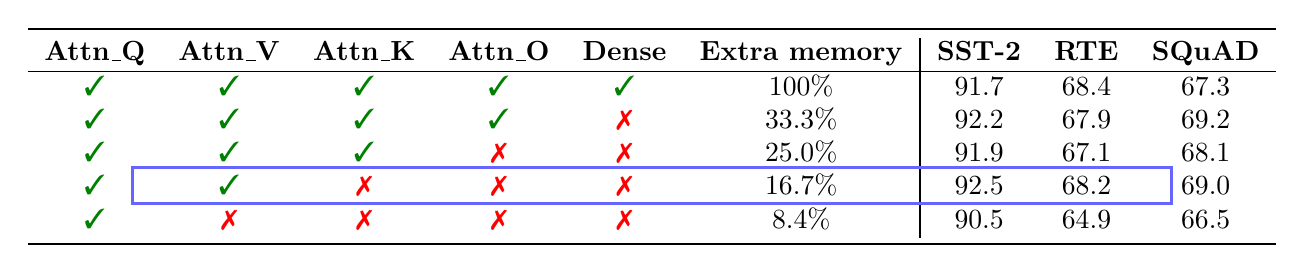
\begin{tikzpicture}
        \node (table) [inner sep=0pt] { % 嵌入表格
            \begin{tabular}{cccccc|ccc}
                \toprule
                \textbf{Attn\_Q} & \textbf{Attn\_V} & \textbf{Attn\_K} & \textbf{Attn\_O} & \textbf{Dense} & \textbf{Extra memory} & \textbf{SST-2} & \textbf{RTE} & \textbf{SQuAD} \\ \hline
                \cmark  & \cmark  & \cmark  & \cmark  & \cmark  & 100\%       & 91.7  & 68.4 & 67.3  \\
                \cmark  & \cmark  & \cmark  & \cmark  & \xmark  & 33.3\%      & 92.2  & 67.9 & 69.2  \\
                \cmark  & \cmark  & \cmark  & \xmark  & \xmark  & 25.0\%      & 91.9  & 67.1 & 68.1  \\
                \cmark  & \cmark  & \xmark  & \xmark  & \xmark  & 16.7\%      & 92.5  & 68.2 & 69.0  \\
                \cmark  & \xmark  & \xmark  & \xmark  & \xmark  & 8.4\%      & 90.5  & 64.9 & 66.5  \\
                \bottomrule
            \end{tabular}
        };

\draw[blue!60!white, very thick] (-6.6, -0.85) rectangle (6.6,-0.4);
    \end{tikzpicture}
    
    \label{ablation_layer}
\end{table*}

\subsection{Ablation for Strategies in ZO Projection Learning}
\label{ablation}


As discussed in Section~\ref{ZO}, we introduce two strategies, \emph{re-initialization} (Re-init) and \emph{projection clipping} (Clipping), to enhance projection learning and improve the stability of fine-tuning. The ablation results for these strategies, along with the corresponding loss curves, are shown in Figure~\ref{ablation_strategy}.

Overall (left in Figure~\ref{ablation_strategy}), omitting either Re-init or Clipping significantly diminishes the benefits of DiZO, with MeZO outperforming DiZO in these cases. Specifically, without Re-init, accuracy drops sharply, falling below MeZO. Similarly, without Clipping, while DiZO slightly outperforms MeZO on simpler datasets like SST-2, it suffers from severe model collapse on more challenging datasets, leading to a significant decline in accuracy.

From the loss curve trajectory (right in Figure~\ref{ablation_strategy}), without Re-init, DiZO loses its advantage in training acceleration, as the loss curve becomes noticeably slower to decrease. Without Clipping, the loss curve exhibits significant oscillations during certain training steps. This instability arises when projections are optimized to unsuitable values, such as extremely large or small magnitudes. These inappropriate projections cause substantial changes in model weights, leading to pronounced oscillations in the loss.

\begin{figure}[h]
\centering
\begin{minipage}{0.48\textwidth}
\scalebox{0.95}{
% \vspace{10pt}
% \begin{tikzpicture}
%         \node (table) [inner sep=0pt] { % 嵌入表格
\begin{tabular}{lcc|ccc}
\toprule
\textbf{Type}                 & \textbf{Re-init} & \textbf{Clipping} &\textbf{SST-2} & \textbf{SNLI}  & \textbf{TREC} \\ \hline
MeZO                  &-         &-          & 90.5  & 66.0 & 76.9  \rule{0pt}{2.5ex} \\ \hline
\multirow{3}{*}{DiZO} &\xmark         &\cmark          & 88.6  & 64.2 & 73.8  \\
                      &\cmark         &\xmark          & 90.9  & 56.2 & 61.2  \\
                      &\cmark         &\cmark          & 92.2  & 71.6 & 77.4  \\
                      \bottomrule
\end{tabular}
% };
}
\vspace{15pt}
% \draw[blue!60!white, very thick] (-3.3, -1.05) rectangle (3.8,-0.65);
% \end{tikzpicture}

\end{minipage}
\begin{minipage}{0.48\textwidth}
        \centering
        \vspace{-10pt}
        \scalebox{0.92}{
        \includegraphics[width=\linewidth]{SST2_loss.pdf}
        }
        \vspace{-14pt}
        % \caption{Experiment result on Llama3-3B and Llama3-8B for four classification
% datasets and one text generation dataset. More results and detailed numbers are in Appendix~\ref{Llama}. }
    \end{minipage}%
    \vspace{5pt}
    \caption{Ablation study for the two strategies: re-initialization and projection clipping, which is conducted on RoBERTa-large ($k=16$). Left: overall results when ablating the strategies. Right: loss curve when ablating the strategies.}
\label{ablation_strategy}
\end{figure}



\subsection{Does Other Alternative Strategies for Layer-wise Divergence Work?}
\label{alternative}

As discussed in Section~\ref{hypo}, our objective is to enhance layer-wise divergence in ZO optimization. Naturally, with consideration of this objective, one may raise two questions regarding the projection strategy we adopt: 1) Can we perform layer-wise projections on the learning rate? 2) When updating weight by projection at $t$-th iteration, why do we use the weights of pre-trained model $\bm{\theta}_0$ as the base of the update (shown in Eq.\ref{equ:4}) instead of the weights from the $(t-1)$-th iteration, $\bm{\theta}_{t-1}$?
% \begin{table}[h]
% \caption{Comparison on conducting projection on learning rate (LR) or use weight at $(t-1)$-th iteration $\bm{\theta}_{t-1}$ instead of the weight of the pre-trained model $\bm{\theta_{0}}$ as the base of projection.}
% \centering
% \begin{tabular}{lccccccccc}
% \toprule
% \multirow{2}{*}{\begin{tabular}[c]{@{}l@{}}Dataset\\ Task Type\end{tabular}} & \textbf{SST-2} & \textbf{RTE} & \textbf{CB} & \textbf{BoolQ} & \textbf{WSC} & \textbf{WIC} & \textbf{MultiRC} & \textbf{SQuAD}       & \textbf{DROP}       \\
%                                                                              & \multicolumn{7}{c}{--------------------------classification--------------------------}                        & \multicolumn{2}{c}{------generation------} \\ \hline
% LR projection                                                                & 56.3           & 54.2         & 50.0        & 47.6           & 36.5         & 52.7         & 44.4             & 29.8                 & 10.0                \\
% $\bm{\theta}_{t-1}$ projection                                                             & 94.2           & 81.2         & 82.1        & 72.2           & 63.8         & 65.8         & 71.6             & 78.4                 & 30.3                \\
% PeZO                                                                         & 94.6           & 80.8         & 82.7        & 77.7           & 59.8         & 64.0         & 72.8             & 77.9                 & 31.1   \\
% \bottomrule
% \end{tabular}
% \label{ablation_projection}
% \end{table}
\begin{table}[h]
\centering
\caption{Comparison on conducting projection on learning rate (LR) or use weight at $(t-1)$-th iteration $\bm{\theta}_{t-1}$ instead of the weight of the pre-trained model $\bm{\theta_{0}}$ as the base of projection. Results are obtained by fine-tuning OPT-2.7B.}
\vspace{5pt}
\begin{tabular}{lcccccc}
\toprule
\multirow{2}{*}{Dataset} & \multicolumn{2}{c}{\textbf{SST-2}}                         & \multicolumn{2}{c}{\textbf{RTE}}                           & \multicolumn{2}{c}{\textbf{SQuAD}}                         \\ \cline{2-7} 
                                                                             & Acc. & \begin{tabular}[c]{@{}c@{}}GPU\\ Hours\end{tabular} & Acc. & \begin{tabular}[c]{@{}c@{}}GPU\\ Hours\end{tabular} & F1.  & \begin{tabular}[c]{@{}c@{}}GPU\\ Hours\end{tabular} \\ \hline
MeZO                                                                         & 90.0 & 100.0\%                                                & 63.5 & 100.0\%                                                & 68.7 & 100.0\%                                                \\
LR projection                                                                & 89.5 & 94.7\%                                                & 63.9 & 108.5\%                                                & 67.9 & 89.8\%                                                \\
$\bm{\theta}_{t-1}$ projection                                                             & 90.7 & 87.8\%                                                & 64.5 & 90.3\%                                                & 67.2 & 88.4\%                                                \\
\rowcolor[gray]{.92}DiZO                                                                         & 92.5 & 55.7\%                                                & 68.2 & 62.3\%                                                & 69.0 & 65.4\%                                                \\ \bottomrule
\end{tabular}
\label{ablation_projection}
\end{table}

To answer the above two questions. We investigate two alternative projection strategies: 1) searching layer-wise ideal learning rate via ZO optimization and then applying the updates, and 2) conducting projection update based on $\bm{\theta}_{t-1}$ instead of $\bm{\theta}_{0}$. Results are illustrated in Table~\ref{ablation_projection}, neither approach achieves performance comparable to DiZO; both yield results closer to MeZO in terms of accuracy and required GPU hours.

% \begin{table*}[]
% \centering
% \scalebox{1}{
% \begin{tabular}{lccccccc}
% \toprule
% Task       & \textbf{\begin{tabular}[c]{@{}c@{}}Gradient\\ free\end{tabular}} & \textbf{\begin{tabular}[c]{@{}c@{}}Parameter\\ efficient\end{tabular}} & \textbf{\begin{tabular}[c]{@{}c@{}}Peak \\ memory\end{tabular}} & \textbf{\begin{tabular}[c]{@{}c@{}}Averaged\\ memory\end{tabular}} & \textbf{Throughput} & \textbf{Iterations} & \textbf{\begin{tabular}[c]{@{}c@{}}GPU \\ hours\end{tabular}} \\ \hline
% MeZO       & \cmark                                            & \xmark                                                  & 13.6 GB                                                      & 13.6 GB                                                        & 3.28 it/s          & 100.0\%                                                            & 100.0\%                                                    \\
% HiZOO      & \cmark                                            & \xmark                                                  & 23.7 GB                                                      & 23.7 GB                                                        & 2.22 it/s          & 59.2\%                                                            & 87.4\%                                                    \\
% \rowcolor[gray]{.92}DiZO       & \cmark                                            & \xmark                                                  & 15.1 GB                                                    & 15.1 GB                                                        & 2.85 it/s          & 51.8\%                                                            & 59.7\%                                                    \\ \hline
% MeZO LoRA  & \cmark                                            & \cmark                                                  & 12.9 GB                                                     & 12.9 GB                                                        & 5.56 it/s          & 74.1\%                                                            & 85.7\%                                                    \\
% HiZOO LoRA & \cmark                                            & \cmark                                                  & 22.9 GB                                                      & 22.9 GB                                                        & 3.70 it/s          & 46.3\%                                                            & 82.0\%                                                    \\
% \rowcolor[gray]{.92}DiZO LoRA  & \cmark                                            & \cmark                                                  & 14.4 GB                                                      & 14.4 GB                                                        & 4.42 it/s          & 38.9\%                                                            & 57.6\%    \\ \hline
% FT         & \xmark                                            & \xmark                                                  & 45.4 GB                                                     & 45.4 GB                                                        & 1.81 it/s          & 9.3\%                                                            & 16.8\%                                                    \\
% LoRA       & \xmark                                            & \xmark                                                  & 18.4 GB                                                     & 18.4 GB                                                        & 4.50 it/s          & 5.6\%                                                            & 4.3\%                                                    \\
% DiZO\textsuperscript{\textdagger}       & \neutral                                          & \xmark                                                  & 17.8  GB                                                     & 15.7 GB                                                        & 2.63 it/s          & 33.3\%                                                            & 41.5\%                                                    \\
% DiZO LoRA\textsuperscript{\textdagger}  & \neutral                                          & \cmark                                                  & 16.1 GB                                                     & 14.7 GB                                                        & 4.16 it/s          & 22.2\%                                                            & 17.5\%                                                    \\
% \bottomrule
% \end{tabular}
% }
% \caption{Memory utilization and speed test on OPT-2.7B on SST-2 dataset (35 tokens per example on average). \neutral: partial gradient-free; \cmark: gradient-free; \xmark: gradient-based. DiZO\textsuperscript{\textdagger}: searching projection with Adam.}
% \label{memory_speed_sst2}
% \end{table*}

\begin{table*}[]
\centering
\caption{Memory utilization and speed test on OPT-2.7B on SST-2 dataset (35 tokens per example on average). \neutral: partial gradient-free; \cmark: gradient-free; \xmark: gradient-based. DiZO\textsuperscript{\textdagger}: searching projection with Adam.}
\vspace{5pt}
\scalebox{1}{
\begin{tabular}{lccccccc}
\toprule
Task Type       & \textbf{\begin{tabular}[c]{@{}c@{}}Gradient\\ Free\end{tabular}} & \textbf{\begin{tabular}[c]{@{}c@{}}LoRA\\ Added\end{tabular}} & \textbf{\begin{tabular}[c]{@{}c@{}}Peak \\ Memory\end{tabular}} & \textbf{\begin{tabular}[c]{@{}c@{}}Averaged\\ Memory\end{tabular}} & \textbf{Throughput} & \textbf{\begin{tabular}[c]{@{}c@{}}\#Train \\ Iter.\end{tabular}} & \textbf{\begin{tabular}[c]{@{}c@{}}GPU \\ Hours\end{tabular}} \\ \hline
FT         & \xmark                                            & \xmark                                                  & 45.4 GB                                                     & 45.4 GB                                                        & 1.81 it/s          & 9.3\%                                                            & 16.8\%                                                    \\
LoRA       & \xmark                                            & \cmark                                                  & 18.4 GB                                                     & 18.4 GB                                                        & 4.50 it/s          & 5.6\%                                                            & 4.3\%                                                    \\
DiZO\textsuperscript{\textdagger}       & \neutral                                          & \xmark                                                  & 17.8  GB                                                     & 15.7 GB                                                        & 2.63 it/s          & 33.3\%                                                            & 41.5\%                                                    \\
DiZO LoRA\textsuperscript{\textdagger}  & \neutral                                          & \cmark                                                  & 16.1 GB                                                     & 14.7 GB                                                        & 4.16 it/s          & 22.2\%                                                            & 17.5\%                                                    \\ \hline
MeZO       & \cmark                                            & \xmark                                                  & 6.8 GB                                                      & 6.8 GB                                                        & 3.28 it/s          & 100.0\%                                                            & 100.0\%                                                    \\
HiZOO      & \cmark                                            & \xmark                                                  & 11.8 GB                                                      & 11.8 GB                                                        & 2.22 it/s          & 59.2\%                                                            & 87.4\%                                                    \\
\rowcolor[gray]{.92}DiZO       & \cmark                                            & \xmark                                                  & 7.5 GB                                                    & 7.5 GB                                                        & 3.05 it/s          & 51.8\%                                                            & 55.7\%                                                    \\ \hline
MeZO LoRA  & \cmark                                            & \cmark                                                  & 6.5 GB                                                     & 6.5 GB                                                        & 5.56 it/s          & 74.1\%                                                            & 43.7\%                                                    \\
HiZOO LoRA & \cmark                                            & \cmark                                                  & 11.5 GB                                                      & 11.5 GB                                                        & 3.70 it/s          & 46.3\%                                                            & 41.0\%                                                    \\
\rowcolor[gray]{.92}DiZO LoRA  & \cmark                                            & \cmark                                                  & 7.2 GB                                                      & 7.2 GB                                                        & 4.92 it/s          & 38.9\%                                                            & 25.9\%    \\ 
\bottomrule
\end{tabular}
}

\label{memory_speed_sst2}
\end{table*}
\begin{table*}[]
\centering
\caption{Memory utilization and speed test on OPT-2.7B on SQuAD dataset (300 tokens per example on average). \neutral: partial gradient-free; \cmark: gradient-free; \xmark: gradient-based. DiZO\textsuperscript{\textdagger}: searching projection with Adam.}
\vspace{5pt}
\scalebox{1}{
\begin{tabular}{lccccccc}
\toprule
Task Type       & \textbf{\begin{tabular}[c]{@{}c@{}}Gradient\\ Free\end{tabular}} & \textbf{\begin{tabular}[c]{@{}c@{}}LoRA\\ Added\end{tabular}} & \textbf{\begin{tabular}[c]{@{}c@{}}Peak \\ Memory\end{tabular}} & \textbf{\begin{tabular}[c]{@{}c@{}}Averaged\\ Memory\end{tabular}} & \textbf{Throughput} & \textbf{\begin{tabular}[c]{@{}c@{}}\#Train \\ Iter.\end{tabular}} & \textbf{\begin{tabular}[c]{@{}c@{}}GPU \\ Hours\end{tabular}} \\ \hline
FT         & \xmark                                            & \xmark                                                  & 73.5 GB                                                      & 73.5 GB                                                        & 0.36 it/s          & 7.5\%                                                            & 27.7\%                                                   \\
LoRA       & \xmark                                            & \cmark                                                  & 58.5 GB                                                      & 58.5 GB                                                       & 0.73 it/s          & 6.3\%                                                            & 11.5\%                                                    \\
DiZO\textsuperscript{\textdagger}       & \neutral                                          & \xmark                                                  & 57.8 GB                                                      & 20.3 GB                                                        & 1.22 it/s          & 41.7\%                                                            & 45.5\%                                                    \\
DiZO LoRA\textsuperscript{\textdagger}  & \neutral                                          & \cmark                                                  & 49.4 GB                                                      & 19.9 GB                                                        & 2.44 it/s          & 31.7\%                                                            & 17.3\%                                                    \\  \hline
MeZO       & \cmark                                            & \xmark                                                  & 8.4 GB                                                      & 8.4 GB                                                        & 1.33 it/s          & 100.0\%                                                            & 100.0\%                                                    \\
HiZOO      & \cmark                                            & \xmark                                                  & 12.3 GB                                                      & 13.3 GB                                                        & 0.97 it/s          & 66.7\%                                                            & 91.5\%                                                  \\
\rowcolor[gray]{.92}DiZO       & \cmark                                            & \xmark                                                  & 9.7 GB                                                      & 9.7 GB                                                        & 1.22 it/s          & 60.0\%                                                            & 65.4\%                                                    \\ \hline
MeZO LoRA  & \cmark                                            & \cmark                                                  & 8.4 GB                                                      & 8.4 GB                                                        & 2.80 it/s          & 73.3\%                                                            & 34.8\%                                                    \\
HiZOO LoRA & \cmark                                            & \cmark                                                  & 11.6 GB                                                      & 12.6 GB                                                        & 2.10 it/s          & 56.7\%                                                            & 35.9\%                                                    \\
\rowcolor[gray]{.92}DiZO LoRA  & \cmark                                            & \cmark                                                  & 9.6 GB                                                      & 9.6 GB                                                        & 2.49 it/s          & 45.0\%                                                            & 24.0\%    \\
\bottomrule
\end{tabular}
}

\label{memory_squad}
\end{table*}

We attribute this phenomenon to the high noise inherent in each ZO update, which relies on random perturbations and thus produces a highly imprecise update direction. In contrast, DiZO projects the optimization direction between the pre-trained and fine-tuned models, and this direction is supposed to be correct. Otherwise, the entire optimization would fail and the loss would not decrease.  Moreover, recent studies suggest that the fine-tuned model is often less robust than their pre-trained version due to catastrophic forgetting~\cite{dong2021should, oh2023towards, zhai2023investigating, wang2024pre}. Maintaining a connection with the pre-trained model helps robustify the fine-tuning process and mitigate some of the noise introduced by ZO’s random perturbations.




% ~\\
% \newpage


% \subsection{PyTorch-style code for gradient-free searching of projections}
% \label{code}




\section{More Experiment Results}

\subsection{Memory and Speed Analysis}
\label{speed}
We present the memory and speed results for OPT-2.7B on the SST-2 and SQuAD datasets in Table~\ref{memory_speed_sst2} and Table~\ref{memory_squad}, respectively. DiZO significantly reduces the number of required iterations while maintaining throughput comparable to MeZO, leading to substantially fewer training GPU hours. In contrast, HiZOO achieves only modest iteration savings and further reduces the throughput of MeZO by approximately 1.5× due to its reliance on second-order information estimation. As a result, HiZOO offers only a slight improvement over MeZO in terms of training GPU hours. In some cases, such as HiZOO combined with LoRA on SQuAD, it even consumes more training GPU hours than MeZO with LoRA.





\subsection{Llama Experiments}
\label{Llama}

To demonstrate the broader applicability of DiZO, we conducted experiments on the Llama-series models. The results for Llama3-3B and Llama3-8B are presented in Table~\ref{Llama-3B} and Table~\ref{Llama-8B}, respectively. DiZO consistently outperforms MeZO across both the 3B and 8B Llama models.

However, we observed that ZO LoRA performs poorly with Llama models (including DiZO, MeZO and HiZOO). The loss value remains stagnant, and the resulting accuracy is comparable to or even worse than zero-shot results. We leave it to future work to investigate why ZO LoRA fails with Llama models. We suspect that this limitation may be related to the Group Query Attention (GQA)~\cite{ainslie2023gqa} mechanism employed in Llama3.
\begin{table*}[h]
\centering
\caption{Experiments results on Llama3-3B for seven classification datasets and two text generation datasets (with 1000 training samples). Better results between MeZO and DiZO are highlighted in bold.}
\vspace{5pt}
\begin{tabular}{lccccccccc}
\bottomrule
\multirow{2}{*}{\begin{tabular}[c]{@{}l@{}}Task\\ Task Type\end{tabular}} & \textbf{SST-2} & \textbf{RTE}  & \textbf{CB}   & \textbf{BoolQ} & \textbf{WSC}  & \textbf{WIC}  & \textbf{MultiRC} & \textbf{SQuAD}       & \textbf{DROP}       \\
                                                                          & \multicolumn{7}{c}{--------------------------classification--------------------------}                             & \multicolumn{2}{c}{------generation------} \\ \hline
% Zero-shot                                                                        & 51.4           & 49.1          & 50.0          & 36.9           & 62.5          & 55.0          & 56.0             & 1.5                 & 0.6                \\
FT                                                                        & 94.2           & 81.2          & 91.4          & 72.2           & 63.8          & 65.8          & 78.2             & 79.6                 & 40.3                \\ \hline
MeZO                                                                      & 88.8           & 67.4          & 73.2          & \textbf{78.0}  & 56.6          & 63.4          & \textbf{64.8}    & 61.9                 & 27.8                \\
\rowcolor[gray]{.92}DiZO                                                                      & \textbf{90.0}  & \textbf{68.2} & \textbf{76.7} & 76.8           & \textbf{57.8} & \textbf{63.8} & 64.2             & \textbf{63.2}        & \textbf{29.7}   \\
\bottomrule
\end{tabular}

\label{Llama-3B}
\end{table*}
\begin{table*}[h]
\centering
\caption{Experiments results on Llama3-8B for seven classification datasets and two text generation datasets (with 1000 training samples). Better results between MeZO and DiZO are highlighted in bold.}
\vspace{5pt}
\begin{tabular}{lccccc}
\toprule
\multirow{2}{*}{\begin{tabular}[c]{@{}l@{}}Task\\ Task Type\end{tabular}} & \textbf{SST-2}   & \textbf{RTE}   & \textbf{CB}   & \textbf{WSC}   & \textbf{SQuAD} \\
                                                                          & \multicolumn{4}{c}{----------classification----------} & --generation-- \\ \hline
MeZO                                                                      & 90.0             & 67.8           & 71.4          & 60.2           & 67.0           \\
\rowcolor[gray]{.92}DiZO                                                                      & \textbf{91.5}             & \textbf{69.4}           & \textbf{73.2}          & \textbf{63.4}           & \textbf{67.4}          \\
\bottomrule
\end{tabular}

\label{Llama-8B}
\end{table*}


\newpage
\section{Proof}
\label{proof}
We consider a neural network with $L$ layers (or parameter blocks) and wish to estimate the gradient of some loss function $\mathcal{L}(\boldsymbol{\theta}; \mathcal{B})$ with respect to all parameters $\boldsymbol{\theta}$. We use a two-point finite-difference (zero-order) method with directions drawn from an isotropic distribution. We show below why the \emph{expected} norm-squared of the resulting gradient estimator is \emph{identical} (or follows the same dimension-based law) for each layer/block.

Consider the $\ell$-th layer. Its estimator is
\[
   \widehat{\nabla_{\boldsymbol{\theta}^{(\ell)}} \mathcal{L}}
   \;=\;
   \frac{1}{q}\,\sum_{i=1}^q
   \Bigl[\,
   \underbrace{
   \frac{
   \mathcal{L}\!\bigl(\boldsymbol{\theta} + \epsilon \boldsymbol{u}_{i}\bigr)
   \;-\;
   \mathcal{L}\!\bigl(\boldsymbol{\theta} - \epsilon \boldsymbol{u}_{i}\bigr)
   }{2\,\epsilon}
   }_{\displaystyle \Delta_i}
   \Bigr]
   \,\boldsymbol{u}_i^{(\ell)},
\]
where $\Delta_i$ is the same scalar for \emph{all} blocks. We want
\[
   \mathbb{E}\Bigl[\|\widehat{\nabla_{\boldsymbol{\theta}^{(\ell)}} \mathcal{L}}\|^2\Bigr].
\]
Note that:
\begin{enumerate}
\item $\Delta_i$ does not depend on $\ell$; it is a single scalar for each direction $i$.
\item $\boldsymbol{u}_i^{(\ell)}$ is the sub-vector of $\boldsymbol{u}_i$ associated to the $\ell$-th block.
\item $\boldsymbol{u}_i$ is drawn from an \emph{isotropic} distribution in $\mathbb{R}^d$, meaning each coordinate has zero mean, unit variance, and there is no cross-correlation between different coordinates. Thus, different blocks $\boldsymbol{u}_i^{(\ell)}$ and $\boldsymbol{u}_i^{(m)}$ (for $\ell \neq m$) are uncorrelated, and each block $\boldsymbol{u}_i^{(\ell)}$ has an identity covariance in its own subspace $\mathbb{R}^{d_\ell}$.
\end{enumerate}

Hence, when we expand 
\[
\|\widehat{\nabla_{\boldsymbol{\theta}^{(\ell)}} \mathcal{L}}\|^2
\;=\;
\Bigl\|
\frac{1}{q}\,\sum_{i=1}^q \Delta_i\,\boldsymbol{u}_i^{(\ell)}
\Bigr\|^2,
\]
the expectation w.r.t.\ $\{\boldsymbol{u}_i\}$ depends on $\ell$ \emph{only} through the dimension $d_\ell$, not through any other distributional asymmetry. If $d_\ell$ are the same for all $\ell$, then the second moment is \emph{literally} the same across all blocks. If $d_\ell$ differ, the dependence is only a (known) function of $d_\ell$.

In short, \textbf{isotropy} ensures that
\[
   \mathbb{E}\!\bigl[\|\widehat{\nabla_{\boldsymbol{\theta}^{(\ell)}} \mathcal{L}}\|^2\bigr]
   \quad
   \text{is the same functional form of }
   \|\nabla_{\boldsymbol{\theta}^{(\ell)}}\mathcal{L}\|^2
   \text{ for each layer } \ell.
\]
Therefore, in the simplest scenario where $d_\ell$ are all the same, each layer gets the \emph{same} second-moment behavior for its gradient estimator.

~\\
\newpage
\section{Implementation}
\label{code}
The following is an implementation of our “ZO projection learning” in PyTorch.

\begin{lstlisting}
def ZO_Projection_Learning(theta_t, theta_0, Gammas, delta, eta, tau, x):
    """
    Perform Zeroth-order Projection Learning.

    Args:
        theta_t: Current model parameters to be fine-tuned.
        theta_0: Pre-trained model parameters (anchor).
        Gammas: Projection parameters need to be optimized.
        delta: Smoothing parameter.
        eta: Learning rate for projection gradient descent.
        tau: Clipping factor for projection bounds.
        x: Input data for the forward pass.
    """
    
    # Calculate the L2 norm of the distance gap
    norms = {
        name: torch.norm(param.data - anchor.data)
        for (name, param), anchor in zip(theta_t.named_parameters(), theta_0.parameters())
    }

    # Initialize the projection values
    for name, gamma in Gammas.named_parameters():
        gamma.data = norms[name]

    for i in range(max_iters):
        # Step 1: Perturb and apply projection, then compute loss
        Gammas = PerturbGamma(Gammas, delta)
        ApplyProjection(theta_t, pre_trained, Gammas)
        loss1 = Forward(theta_t, x)
        ReverseProjection(theta_t)  # Reset the parameter before projection

        # Step 2: Reverse and apply projection, then compute loss
        Gammas = PerturbGamma(Gammas, -2 * delta)
        ApplyProjection(theta_t, pre_trained, Gammas)
        loss2 = Forward(theta_t, x)
        ReverseProjection(theta_t)  # Reset the parameter before projection

        # Step 3: Reset projection and compute gradient
        Gammas = PerturbGamma(Gammas, delta)  # Reset projection
        grad = (loss1 - loss2) / (2 * delta)

        # Step 4: Gradient descent with clipping
        for name, gamma in Gammas.named_parameters():
            torch.manual_seed(seed)  # For resampling perturbation
            z = torch.normal(mean=0, std=1, size=gamma.data.size())
            gamma.data = torch.clip(
                gamma.data - eta * grad * z,
                (1 - tau) * norms[name],
                (1 + tau) * norms[name],
            )  # Conduct descent and apply clipping

    return Gammas

\end{lstlisting}



% %%%%%%%%%%%%%%%%%%%%%%%%%%%%%%%%%%%%%%%%%%%%%%%%%%%%%%%%%%%%%%%%%%%%%%%%%%%%%%%
% %%%%%%%%%%%%%%%%%%%%%%%%%%%%%%%%%%%%%%%%%%%%%%%%%%%%%%%%%%%%%%%%%%%%%%%%%%%%%%%
% % APPENDIX
% %%%%%%%%%%%%%%%%%%%%%%%%%%%%%%%%%%%%%%%%%%%%%%%%%%%%%%%%%%%%%%%%%%%%%%%%%%%%%%%
% %%%%%%%%%%%%%%%%%%%%%%%%%%%%%%%%%%%%%%%%%%%%%%%%%%%%%%%%%%%%%%%%%%%%%%%%%%%%%%%
% \newpage
% \appendix
% \onecolumn
% \section{You \emph{can} have an appendix here.}

% You can have as much text here as you want. The main body must be at most $8$ pages long.
% For the final version, one more page can be added.
% If you want, you can use an appendix like this one.  

% The $\mathtt{\backslash onecolumn}$ command above can be kept in place if you prefer a one-column appendix, or can be removed if you prefer a two-column appendix.  Apart from this possible change, the style (font size, spacing, margins, page numbering, etc.) should be kept the same as the main body.
% %%%%%%%%%%%%%%%%%%%%%%%%%%%%%%%%%%%%%%%%%%%%%%%%%%%%%%%%%%%%%%%%%%%%%%%%%%%%%%%
% %%%%%%%%%%%%%%%%%%%%%%%%%%%%%%%%%%%%%%%%%%%%%%%%%%%%%%%%%%%%%%%%%%%%%%%%%%%%%%%


\end{document}

